\documentclass[12px]{article}
\usepackage[utf8x]{inputenc}
\usepackage[portuges]{babel}
\usepackage[svgnames]{xcolor}
\usepackage{graphicx}
\usepackage{a4wide}
\usepackage{float}
\usepackage[export]{adjustbox}
\usepackage{spverbatim}
\usepackage{hyperref}
\usepackage{enumitem}
\usepackage{indentfirst}
\usepackage{lscape}

\setdescription{leftmargin=\parindent,labelindent=\parindent}

\newcommand*{\plogo}{\fbox{$\mathcal{PL}$}}
\newcommand*{\titleTH}{\begingroup
\raggedleft
\vspace*{\baselineskip}

{\Large Universidade do Minho}\\[0.167\textheight]
{\LARGE\bfseries Projeto Integrado}\\[\baselineskip]
{\Huge Gestão de Trabalhos Práticos}\\[\baselineskip]
{\Large \textit{Engenharia de Linguagens 13/14}}\par

\vfill

\Large{André Santos pg25329\\Daniel Carvalho a61008\\Ricardo Branco pg25339}\par

\vspace*{3\baselineskip}
\endgroup}

\begin{document}
\thispagestyle{empty}
\titleTH
\newpage

\begin{abstract}

  Este relatório cobre todo o processo de planeamento, desenvolvimento e
  documentação de um sistema que resolva um problema abordado na UCE de
  Engenharia de Linguagens na forma de Projeto Integrado, nomeadamente
  a gestão de trabalhos práticos académicos desde a sua criação pelos docentes, à resolução pelos alunos
  e à publicação dos mesmos ao resto da comunidade \textit{online}.

  A abordagem na resolução deste projeto passa por aliar todos os conhecimentos
  adquiridos nos módulos integrantes de Engenharia de Linguagens, passando por
 Engenharia Gramatical, \textit{Scripting} no Processamento de Linguagem Natural, Processamento
 Estruturado de Documentos e Análise e Transformação de Software.

 Neste sentido pretende-se aliar ao desenvolvimento deste sistema conhecimentos
 como gramáticas de atributos, ambientes de desenvolvimento estruturais e
 orientados à semântica, representação de manipulação de conhecimento com
 eficiência, automatização de tarefas e transformações, utilização de expressões
 regulares, linguagens DSL, corpora, automatização de testes para diferentes
 linguagens de programação, manipulação de documentos estruturados, utilização
 de XML, XSL e XSL-FO, documentos anotados, publicação de conhecimento na web,
 entre outros.

\end{abstract}

\newpage

\tableofcontents
\newpage

\section{Introdução}

Em termos gerais, este projeto baseia-se num sistema de informação que permita a gestão de trabalhos 
práticos de unidades curriculares de alunos do ensino superior.

A ideia central é permitir receber os trabalhos (programa e relatório) entregues por cada grupo e 
permitir associar a cada submissão os comentários e a classificação atribuída pelo docente, 
permitindo gerar a pauta da turma. No entanto de forma a garantir um maior 
espetro de usabilidade, olhar para o sistema de forma a poder suportar 
trabalhos práticos num formato mais genérico que permita não só receber 
trabalhos de programação mas todo o tipo de trabalhos práticos produzidos.
Não obstante, no que diz respeito aos trabalhos de programação, serão tidas em 
atenção algumas funcionalidades que melhorem o tratamento deste tipo específico 
de trabalhos fornecendo ferramentas para testes automáticos ao código submetido 
pelos alunos, que avaliam o funcionamento desejado ou não consoante as 
especificações do docente.

Para este sistema ser completo e funcional deve também garantir funcionalidades como
a gestão de unidades curriculares e a sua equipa docente,  gestão de turnos e dos alunos inscritos, e a
criação de trabalhos práticos dentro da unidade curricular.

No que diz respeito à implementação, este sistema é suportado por uma aplicação \textit{web}, acessível
nos vários tipos de dispositivos (computador, \textit{tablet}, \textit{smartphone}), deverá garantir a persistência de 
dados numa base de dados relacional, deverá garantir a interoperabilidade com outros sistemas para
importação ou exportação de dados, bem como permitir a publicação de pautas em vários formatos.

Noutra perspetiva é necessário tratar os trabalhos práticos disponibilizados na aplicação
e criar um sistema que sirva de repositório digital dos mesmos. Na sua implementação é necessário
garantir um \textit{backoffice} que permita aos professores fazer a gestão das unidades curriculares
de que são responsáveis, assim como dos turnos e projetos da mesma. É também requerido garantir
aos alunos a gestão dos seus grupos dentro dos projetos, assim como garantir a funcionalidade
de entrega de trabalhos práticos.
 
 Por fim, torna-se imperativo garantir a todos os utilizadores do sistema, a possibilidade de procura
 e consulta de todos os projetos disponíveis para o público.
 
 Posto isto, o sistema deve ter como a estrutura do modelo de referência internacional OAIS 
 (\textit{Open Archive Information System}).
 Nesta estrutura existem três organismos que fazem funcionar o sistema. Os produtores, que 
 alimentam o sistema com os trabalhos práticos, os administradores que fazem a gestão e administração
 dos trabalhos práticos e os consumidores que irão usufruir dos trabalhos práticos. 
 
No que concerne à validação dos projectos submetidos há a necessidade de verificações e 
criação de um modelo genérico a que todas as submissões terão de obedecer. Neste processo
é necessário tratar-se do SIP (\textit{Submission Information Package}) na ingestão do sistema dos
trabalhos práticos, que após tratamento da informação se transforma num AIP (\textit{Archival 
Information Package}) e então arquivado, e por fim a aplicação disponibiliza o trabalho no formato
de um DIP (\textit{Dissemination Information Package}) pronto a ser disseminado e consumido pelos
utilizadores do sistema.

\newpage

\section{Plano de trabalho}

Tendo em conta a dimensão da aplicação, foi criado um plano de trabalho onde se mapearam as tarefas
de desenvolvimento no tempo de forma contínua, tornando assim possível adaptar um ritmo de trabalho
consistente com os prazos de entrega de cada fase e então cumprir as metas do projeto.

Nesse sentido dividiu-se o projeto em três fases, sendo elas o \textbf{planeamento e análise de requisitos}, o
\textbf{desenvolvimento} e a \textbf{documentação}.

No que diz respeito à fase de planeamento e análise de requisitos, esta fase engloba todo o levantamento 
de funcionalidades assim como todo o planeamento e estruturação do projeto 
nomeadamente, criação do modelo de domínio, diagrama de classes, modelação do repositório de dados,
análise da concorrência, plano de trabalho, plano tecnológico, casos de estudo, arquitetura do sistema, etc.

Para esta fase de planeamento, análise e modelação foi criado um plano de um mês onde todas as tarefas 
teriam de estar concluídas. Na Figura \ref{fig: workplan1} é possível ver um diagrama de Gantt com
o planeamento inicial.

\begin{figure}[H] 
  \centering
  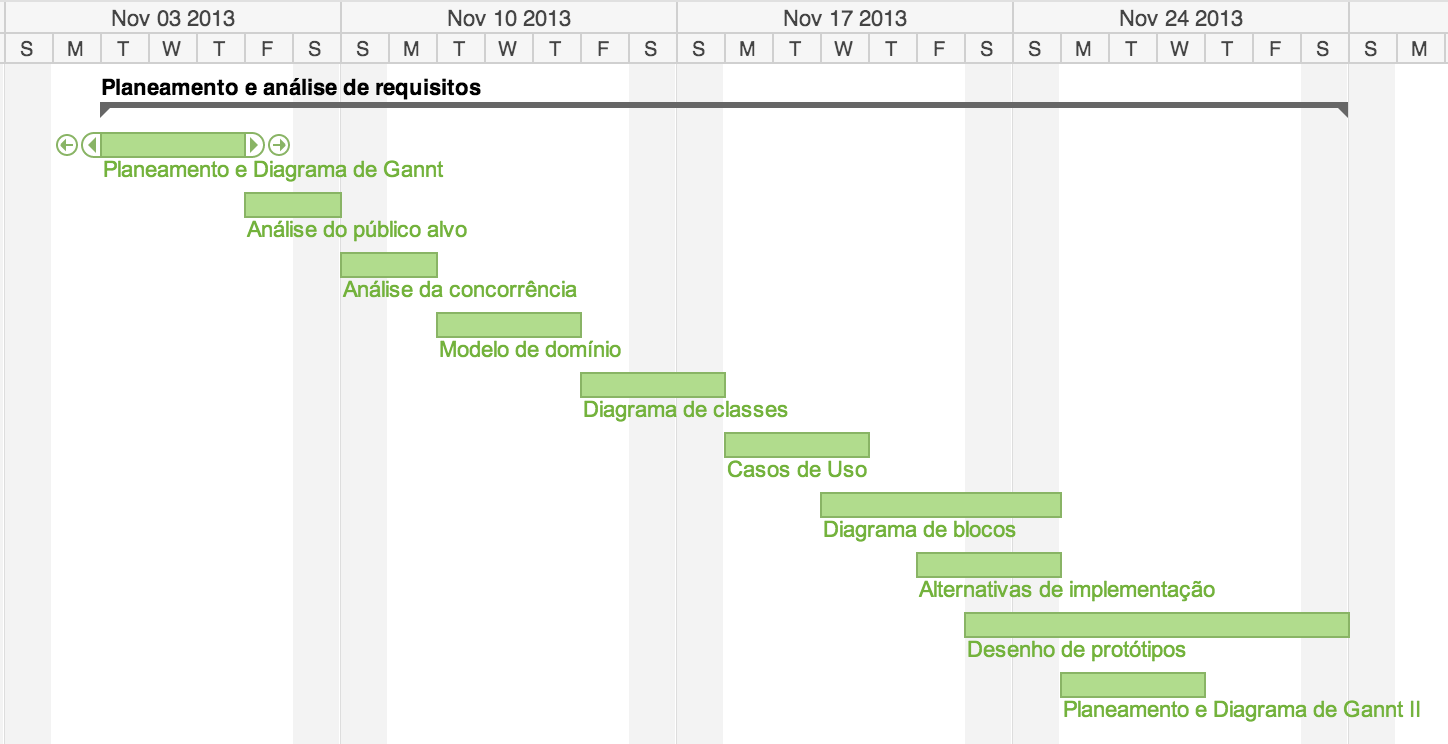
\includegraphics[width=1\textwidth]{images/plano_de_trabalho/gannt_1.png}
  \caption{Diagrama de Gantt para o planeamento e análise de requisitos}
  \label{fig: workplan1}
\end{figure}

De seguida, prosseguindo para o planeamento da fase de desenvolvimento após 
analisar as funcionalidades e modelar o sistema  é altura de começar a 
prototipar a aplicação e começar a iterar sobre as funcionalidades a 
implementar. Neste sentido englobaram-se aqui tarefas como prototipagem em HTML, 
criação de migrações na modelação da base dados, modelação das entidades a 
representar (modelos) na forma da arquitetura MVC seguindo-se a implementação dos 
controladores e visões, tendo como base as funcionalidades a desenvolver para o 
sistema. Nesta fase pretende-se tornar a aplicação capaz de suportar os seus 
utilizadores (não registados, docentes e alunos) das tarefas de gestão de UCs, 
projetos, grupos e submissões, assim como consulta e disponibilização de 
projetos. No que diz respeito à metodologia de desenvolvimento seguir-se-ão 
os métodos e princípios de desenvolvimento de software \textit{Agile}. Posto isto, 
far-se-á um desenvolvimento cíclico e iterativo focado em cada grupo de 
funcionalidades, desenvolvendo-as, testando-as e validando-as. Caso seja 
necessário fazer novas iterações sobre um grupo de funcionalidades, basta 
repetir o ciclo até que seja possível validar o que foi desenvolvido e de seguida inicia-se 
um novo ciclo de desenvolvimento para o grupo de funcionalidades seguinte.

Desta forma é possível uma rápida adaptação a mudanças e ajustes sem ter que verificar e 
revalidar todo o planeamento inicial do projeto e ainda assim atingir as metas 
definidas.

Faça-se notar que em cada ciclo de desenvolvimento para além da implementação,
 serão feitos testes de usabilidade e funcionalidade, dessa forma é possível garantir que em cada estado do 
desenvolvimento, todas as funcionalidades implementadas encontram-se o mais perto 
do idealizado possível.
Durante cada ciclo de desenvolvimento também faremos a integração da 
documentação relativa ao grupo de funcionalidades que estão a ser implementadas.
É possível ver nas Figuras \ref{fig: workplan2}, \ref{fig: workplan3}, \ref{fig: workplan4} 
os diagramas de Gantt com o planeamento respetivo à fase de desenvolvimento.

\begin{figure}[H] 
  \centering
  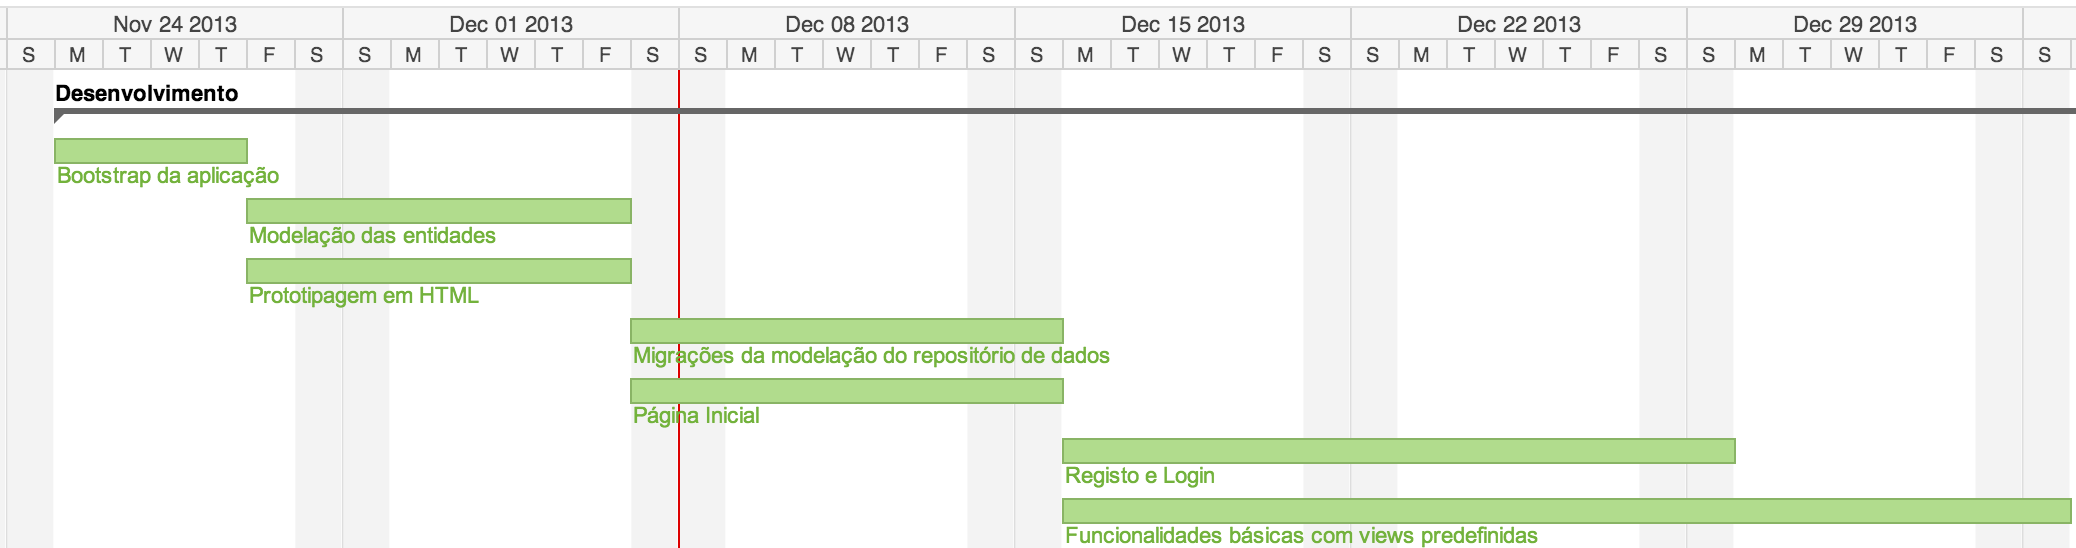
\includegraphics[width=1\textwidth]{images/plano_de_trabalho/gannt_2.png}
  \caption{Diagrama de Gantt para o desenvolvimento I}
  \label{fig: workplan2}
\end{figure}

\begin{figure}[H] 
  \centering
  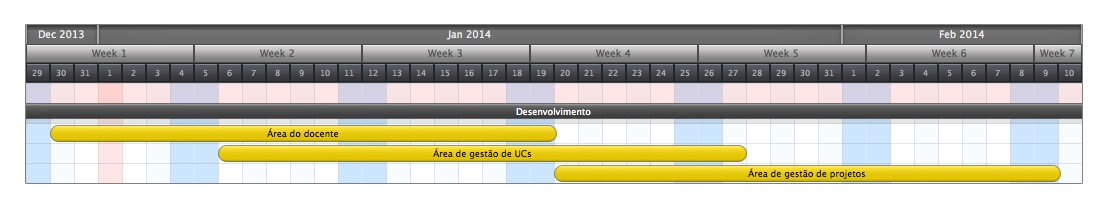
\includegraphics[width=1\textwidth]{images/plano_de_trabalho/gannt_3.png}
  \caption{Diagrama de Gantt para o desenvolvimento II}
  \label{fig: workplan3}
\end{figure}

\begin{figure}[H] 
  \centering
  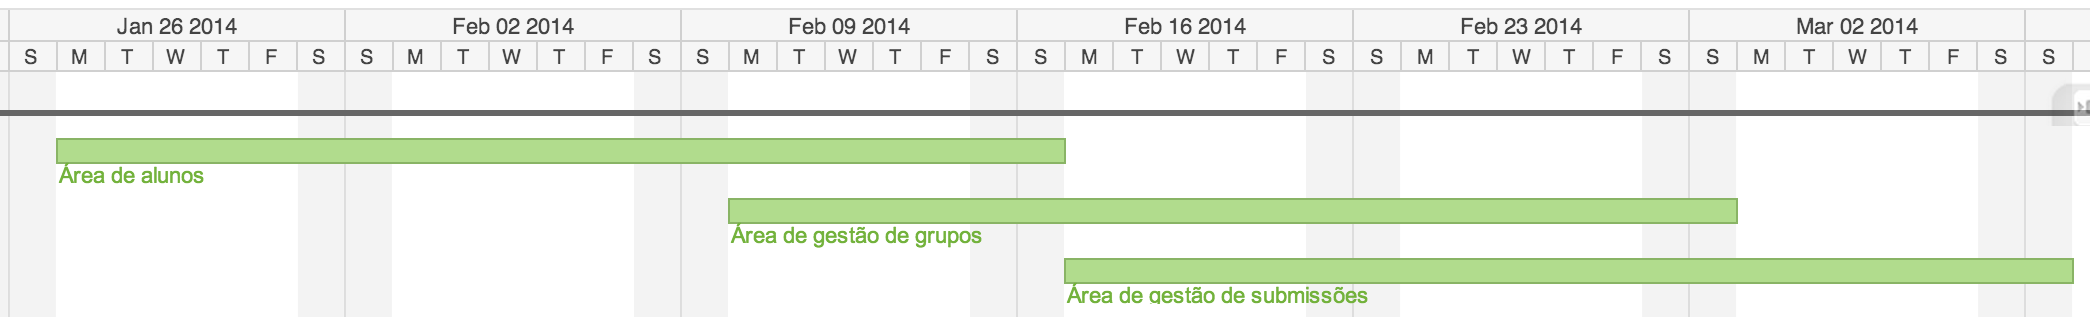
\includegraphics[width=1\textwidth]{images/plano_de_trabalho/gannt_4.png}
  \caption{Diagrama de Gantt para o desenvolvimento III}
  \label{fig: workplan4}
\end{figure}

Por fim, terminámos com a fase de documentação onde será feita toda a descrição 
do sistema desenvolvido em termos de funcionalidades e implementação de forma a 
possibilitar a consulta tanto aos interessados em utilizar a aplicação bem como 
de forma a suportar a possível necessidade de manutenção da aplicação. Desta 
forma qualquer um pode entender todo o sistema na sua plenitude através da 
documentação criada. As tarefas desta fase serão distribuídas pelos ciclos de 
desenvolvimento falados acima, em que cada fase de documentação será empregue no 
mesmo ciclo de desenvolvimento das funcionalidades respetivas.

O diagrama de Gantt completo encontra-se representado em Anexo na Figura \ref{fig: 
workplan0}.

\newpage

\section{Análise do problema}

No meio académico, principalmente em áreas mais focadas numa vertente prática, muitas vezes
os alunos são postos à prova através de trabalhos práticos. Neste caso, após a avaliação, os trabalhos
práticos são arquivados pelos docentes e esquecidos permanentemente numa prateleira, até um dia
serem deitados fora.

No sentido de promover a investigação e a partilha de conhecimento, torna-se não só necessário
criar uma plataforma de gestão de disciplinas universitárias e os seus trabalhos práticos, como também
tornar possível a partilha de todo o conhecimento que é inevitavelmente inerente aos resultados
do desenvolvimento destes.

No momento as ferramentas que existem no mercado, se por um lado permitem toda a gestão de
unidades curriculares de uma universidade, pecam por se focarem por um funcionamento fechado
para dentro da instituição e consequentemente fechado para dentro dos cursos e das unidades curriculares.
Nesse sentido o sistema retratado neste relatório, preenche a lacuna existente entre o que é desenvolvido
num âmbito académico e o resto da população.

Como resultado deste tipo de ponte entre os dois mundos, espera-se conseguir manter uma plataforma
que não só incentive a investigação tanto dentro do mundo académico, como profissional e individual,
como também incentive a partilha de conhecimento e fomente o desenvolvimento das
áreas de atuação condizentes com cada trabalho prático disponível na
plataforma.

Para além disso, torna-se imperativo criar um modelo genérico de publicação de
trabalhos práticos para dessa forma se tornar muito mais acessível o consumo de
informação para os utilizadores da plataforma.

No entanto também se torna necessário o foco no lado mais académico e das
necessidades dos docentes e alunos. Neste sistema todo o processo de
interatividade entre os utilizadores e a aplicação, permite tanto aos docentes
como aos alunos realizarem a gestão das suas unidades curriculares e trabalhos
práticos criando assim um sistema que cumpre as necessidades académicas internas dos docentes
e alunos bem como estabelece um ponto de ligação entre a comunidade académica e
o trabalho desenvolvido nesse meio, e o resto das pessoas com interesse nas
áreas abrangidas pelos projetos disponíveis.

\newpage

\section{Análise de requisitos}

Identificado o problema, pretende-se assim desenvolver um sistema de informação para gestão de trabalhos práticos. O sistema oferecerá um conjunto de funcionalidades e facilidades aos docentes e alunos em todo o processo de entrega de um trabalho prático, desde a gestão da unidade curricular até à publicação das avaliações.

Identifica-se à partida 3 grupos de utilizadores com funcionalidades e objetivos diferentes em todo o processo.

O primeiro grupo de utilizadores são os \textbf{alunos}, para estes pretende-se oferecer a possibilidade de submeterem projetos práticos de uma forma simples e facilitada. As submissões poderão ser efetuadas individualmente ou em grupos conforme o especificado pelo docente. O aluno terá acesso a um painel de gestão das suas unidades curriculares e projetos, poderá consultar todas as informações de um projeto e respetivas fases, gerir facilmente os seus grupos de trabalho, consultar o seu histórico de entregas e consultar em diferentes formatos as suas avaliações dos projetos e/ou fases. Pretende-se ainda que o aluno tenha a possibilidade de ser notificado de todas as alterações nos projetos que faz parte, através de avisos do sistema ou emails. Estas notificações serão também importantes para informar o aluno da aproximação dos prazos de entrega dos projetos das suas unidades curriculares.

No processo de submissão de um projeto, o sistema, deverá ser capaz de facilitar a criação do \textit{Project Record} do pacote enviado, assim como identificar e notificar falhas na submissão, tais como não conter todos os ficheiros obrigatórios ou não gerar o executável pretendido. Neste caso os alunos poderão receber no email essa informação para assim submeterem uma versão corrigida.
Um aluno terá também a possibilidade de tornar o projeto desenvolvido público.

O segundo grupo de utilizadores são os \textbf{docentes}, numa primeira componente estes utilizadores poderão criar e gerir unidades curriculares e todas as informações adjacentes a estas, um docente de uma unidade curricular pode adicionar docentes responsáveis, adicionar alunos e associá­-los a diferentes turnos. Dentro da gestão de uma unidade curricular um docente será capaz de criar projetos devidamente documentados (organizados ou não em diferentes fases), podendo ainda especificar ficheiros obrigatórios, executável obrigatório e ficheiros de teste para facilitar a correção dos mesmos. Estes testes serão executados no programa enviado e serão guardadas as diferenças do output obtido para o output esperado. Dentro do painel de gestão de um projeto o docente poderá consultar as entregas dos diferentes grupos e avaliar as entregas por grupo ou individualmente. Depois de avaliadas as entregas, o docente, poderá gerar automaticamente as pautas do projeto e/ou fase e publicar para os alunos da unidade curricular.
Numa fase final, o docente poderá tornar o projeto (enunciado e especificações do problema) público.

Para além dos docentes e dos alunos, o nosso sistema permitirá uma procura e consulta de projetos públicos desenvolvidos a \textbf{utilizadores não registados}.

Pretende-se no desenvolvimento do sistema simplificar todas as tarefas dos utilizadores alvo do sistema, e proporcionar um sistema flexível que possa ser utilizado por um abrangente número de utilizadores.

Nesse seguimento o sistema procurará ser flexível, não se restringindo a apenas uma abordagem nem sendo demasiado genérico, procurar-se-á definir abordagens mais específicas, mas sempre com opções mais genéricas para englobar casos menos comuns. É exemplo disso a geração automática do \textit{Project Record} do pacote enviado, em casos mais específicos o ficheiro poderá ser entregue pelo utilizador, no entanto em outros casos torna-se necessário auxiliar na geração desse mesmo ficheiro para assegurar que todos os pacotes enviados estão em conformidade com a estrutura esperada de um pacote. O sistema também procurará simplificar processos organizacionais, como facilitar a criação de uma unidade curricular identificando apenas nome, instituição, curso e ano letivo. O facto de uma unidade curricular estar associada a um ano letivo ajuda a nível organizacional e permite que não seja necessária a transferência de alunos e docentes entre anos letivos. Procurará também simplificar processos de validação das entregas através das restrições de ficheiros obrigatórios e nome do executável. Ser capaz de automatizar a avaliação através dos testes no sistema e geração de pautas automáticas e de gerir mais facilmente grupos de trabalho e respetivas entregas.

O objetivo final é lançar um sistema bem focado onde cada grupo de utilizadores execute com facilidade as suas tarefas principais, perdendo o menor tempo possível em problemas secundários.

\newpage

\section{Concorrência e alternativas}

Uma das medidas efetuadas durante o planeamento da aplicação foi a análise de concorrência e o estudo das alternativas existentes. Desta forma foi possível adicionar mais funcionalidades à aplicação de forma a que esta fosse o mais completa possível.

\subsection{Concorrência}
\label{sub:concorrencia}

De todas as aplicações concorrentes, as que mais se destacam são os Sistemas de Gestão de Aprendizagem (\emph{SGA}),também conhecidas por \emph{Learning Management Systems} - \emph{LMS}. Dentro dos \emph{SGA} imperam as seguintes aplicações:
\begin{itemize}
	\item \emph{Blackboard}
	\item \emph{Moodle}
	\item \emph{Studifi}
	\item \emph{Haiku LMS}
\end{itemize}

\subsubsection{Blackboard}
\label{ssub:blackboard}

\begin{figure}[H]
        \centering
        
\includegraphics[width=0.5\textwidth]{images/concorrencia/blackboard.jpg}
         \caption{\emph{Blackboard}}
         \label{fig: blackboard}
\end{figure}

A aplicação \href{http://www.blackboard.com}{\emph{Blackboard}} é composta por quatro tipos de utilizadores:
\begin{description}
	\item[Aluno] Um aluno pode submeter projetos, inscrever-se em grupos e consultar a informação disponibilizada pelos professores.
	\item[Professores] Um professor pode criar projetos e fazer avaliações qualitativas e quantitativas dos trabalhos enviados. Os projetos criados podem ter correção automática.
	\item[Técnicos] Os técnicos são responsáveis pela manutenção da aplicação.
	\item[Supervisores] Os supervisores fazem a gestão de cursos, disciplinas, docentes e alunos. Estes também podem gerar estatísticas do sistema.
\end{description}

Os projetos criados na \emph{Blackboard} não estão disponíveis para o público. Também não existe a noção de turnos, sendo estes substituídos pelos grupos. Os grupos são criados dentro da disciplina e um aluno pode estar inscrito em múltiplos grupos.

\subsubsection{Moodle}
\label{ssub:moodle}
\begin{figure}[H]
        \centering
        
\includegraphics[width=0.5\textwidth]{images/concorrencia/moodle.jpg}
         \caption{\emph{Moodle}}
         \label{fig: moodle}
\end{figure}
A aplicação \href{http://www.moodle.org}{\emph{Moodle}} é composta por três tipos de utilizadores:

\begin{description}
	\item[Alunos] Os alunos podem submeter projetos e consultar a informação disponibilizada pelos professores.
	\item[Professores] Os professores podem criar projetos e fazer uma avaliação quantitativa dos projetos enviados. Os projetos criados podem ter correção automática.
	\item[Administradors] Os Administradores são responsáveis pela manutenção da aplicação. Também são responsáveis por fazer a gestão dos utilizadores existentes.
\end{description}


Um dos problemas do \emph{Moodle} é a inexistência de grupos e de turnos. Quanto a projetos públicos apenas se estes forem inseridos manualmente pelos alunos nos seus portefólios.

\subsubsection{Studifi}
\label{ssub:studifi}

\begin{figure}[H]
        \centering
        
\includegraphics[width=0.5\textwidth]{images/concorrencia/studifi.png}
         \caption{\emph{Studifi}}
         \label{fig: studifi}
\end{figure}

A aplicação \href{https://studifi.com/}{\emph{Studifi}} é composta por três tipos de utilizadores:

\begin{description}
	\item[Alunos] Os alunos podem submeter projetos e consultar a informação disponibilizada pelos professores.
	\item[Professores] Os professores podem criar exercícios que são avaliados automaticamente e podem criar projetos.
	\item[Administradors] Os Administradores são responsáveis pela manutenção da aplicação. Também são responsáveis por fazer a gestão dos utilizadores existentes.
\end{description}

No \emph{Studifi} os exercícios não estão disponíveis para o público. Uma das características que se destaca nesta aplicação é a existência de controlo de versões nos ficheiros submetidos.

\subsubsection{Haiku LMS}
\label{ssub:haiku_lms}

\begin{figure}[H]
        \centering
        
\includegraphics[width=0.5\textwidth]{images/concorrencia/haiku.png}
         \caption{\emph{Haiku LMS}}
         \label{fig: studifi}
\end{figure}

A aplicação \href{http://www.haikulearning.com/}{\emph{Haiku LMS}} é composta por três tipos de utilizadores:

\begin{description}
	\item[Alunos] Os alunos podem submeter projetos e consultar a informação disponibilizada pelos professores.
	\item[Professores] Os professores podem criar projetos e exercícios e gerir pautas de avaliação.
	\item[Instituições de ensino] Responsáveis pela gestão de cursos e disciplinas da instituição.
\end{description}

\subsection{Alternativas}
\label{sub:alternativas}

No que diz ao respeito às alternativas, estas são divididas em cinco situações:
\begin{itemize}
	\item Submissão de trabalhos

	\begin{description}
		\item[Submissão via \emph{mail}] O aluno envia um \emph{mail} com o trabalho para o \emph{mail} de um docente. Muitas vezes com um assunto especifico para que o docente possa filtrar o \emph{mail} e obter os vários trabalhos enviados.
		\item[Partilha de \emph{links}] O aluno faz \emph{upload} do seu trabalho para um servidor externo(\emph{github,dropbox,etc}) e partilha o \emph{link} com o docente.
		\item[Entrega de unidades de armazenamento] O aluno grava o seu trabalho numa unidade de armazenamento(\emph{Usb flash drive, cd/dvd, etc}) e entrega a respetiva unidade ao docente.
	\end{description}

	\item Gestão de pautas

	\begin{description}
		\item[Folhas de cálculo ou \emph{PDF}] É entre aos alunos um ficheiro com as notas do projeto. Muitas vezes a pauta entregue não refere a qualidade do trabalho.
		\item[Vitrinas] O docente imprime as notas finais e afixa-as numa vitrina do estabelecimento de ensino.
	\end{description}

	\item Correção automática

		\begin{description}
			\item[Script] Fica ao critério do docente, as funcionalidades desse emph{script}, isto é se o emph{script} criado verifica por exemplo extensões de ficheiros ou até mesmo se os ficheiros enviados correspondem a um determinado emph{output} para um certo \emph{input}.
		\end{description}
	\item Inscrições de grupos

	\begin{description}
		\item[\emph{Mail}] Um responsável do grupo envia um \emph{mail} ao docente com a constituição do grupo. Este \emph{mail} pode ficar sujeito as mesma regras que a submissão de trabalhos via \emph{mail}.
		\item[Entrega do trabalho] O grupo só fica registado e o docente só tem conhecimento desta após a entrega do trabalho.
		\item[Aviso com presença] Um elemento do grupo ou então todos os elementos notificam o docente em frente deste.
	\end{description}

	\item Gestão de grupos

	\begin{description}
		\item[Documento] O docente possui um documento com a constituição dos grupos e de outras informações relativas a esse grupo como por exemplo as notas dos trabalhos
	\end{description}

\end{itemize}

\newpage

\section{Casos de estudo}
De forma a verificar a viabilidade da aplicação decidiu-se usar três casos reais. Nesse sentido irá se explorar cada um dos casos de forma a explorar como a aplicação resolve os problemas expostos.

\subsection{Engenharia de Linguagens}
\label{sub:engenharia_de_linguagens}

No primeiro caso tem-se o Projeto Integrado de Engenharia de Linguagens do Mestrado em Engenharia Informática da Universidade do Minho.
Engenharia de Linguagens tem um turno e quatro docentes.

Quanto ao Projeto Integrado, este tem que ser feito por grupos com o máximo de três elementos. Existem quatro fases de entrega (as 3 primeiras tem uma nota qualitativa e a última fase vale 20 valores). Relativamente à entrega, em cada fase é obrigatório entregar um relatório e um conjunto de slides usados na apresentação. Na última fase além do relatório, torna-se obrigatório enviar o código desenvolvido assim como outros ficheiros que o grupo ache relevante.

O processo começa com o registo do docente responsável, caso o docente já possua uma conta tem de efetuar \emph{login} na aplicação. Após o \emph{login} é necessário criar a cadeira de Engenharia de Linguagens, durante este processo será necessário preencher campos relativos ao nome da instituição e do curso. Caso já  exista o curso ou a instituição, a disciplina será associada aos campos existentes. No fim de criar a disciplina, o docente será encaminhado para o painel da disciplina criada. Dentro do painel da disciplina, o docente responsável pode adicionar docentes à disciplina.

Procede-se para a criação do projeto. Ao criar um novo projeto o docente adiciona o enunciado, adiciona as várias fases do projeto, indica que os grupos só podem ter três elementos. Em cada fase indica que tem que ser enviado um relatório e os \emph{slides} da apresentação em formato \emph{PDF}. Por fim tem a opção de lançar o projeto ou se apenas o quer deixar visível para o resto da equipa docente, para o caso de haverem alterações. Após o projeto estar criado o docente é encaminhado para o painel do projeto.
Um aluno uma vez registado e autenticado inscreve-se na cadeira e acede ao painel do projeto. No painel do projeto cria o seu grupo e faz uma submissão. É então reencaminhado para um formulário onde escreve um resumo do trabalho feito e envia os ficheiros necessários, concluindo assim a submissão.

Voltando ao docente, este acede novamente ao painel do projeto e abre a página de entrega de um projeto submetido. Após analisar o relatório ou qualquer outro ficheiro enviado, carrega em avaliar e atribui a nota ao grupo ou a cada elemento individualmente, podendo também adicionar comentários sobre a nota atribuída.

\subsection{Estatística}
\label{sub:estat_stica}

No segundo caso tem-se como exemplo um projeto da cadeira de Estatística do curso de Economia. Esta cadeira tem quatro turnos e dois docentes. Quanto ao projeto tem que ser feito em grupos de dois ou três elementos, restringido a alunos do mesmo turno, tem apenas uma fase, existe um ficheiro com dados para auxilio da realização do projeto e no momento da entrega além do relatório tem-se que enviar os resultados obtidos no \emph{SPSS} que estão no formato \emph{SAV}.

O processo começa pelo registo da cadeira no sistema após o registo e identificação do docente. Assumindo que todos os alunos já se inscreveram na disciplina é feito a inscrição dos alunos em cada turno por parte do docente. De seguida cria-se o projeto no qual se indica o enunciado do projeto, o ficheiro de dados, restringe-se os grupos para que estes sejam constituídos por elementos do mesmo turno e que a dimensão deste seja de dois a três elementos e indica-se quais os ficheiros obrigatórios no momento da entrega. Por último os alunos submetem o projeto feito e o docente indica a nota do mesmo tal como acontece no primeiro caso.

\subsection{Desafios de Proramação da Universidade do Minho}
\label{sub:desafios_de_prorama_o_da_universidade_do_minho}

No terceiro e último caso pretende-se submeter os desafios algorítmicos dos Desafios de Programação da Universidade do Minho (DPUM). Estes desafios são feitos individualmente e são corregidos automaticamente pela aplicação. Não é necessário entregar relatório e não existe data limite de submissão.

Quanto aos Desafios de Programação da Universidade é dirigido por um único docente e não existem turnos. Na submissão de um desafio é obrigatório que haja uma \emph{Makefile} e que o nome do executável deverá ser igual o ao nome indicado pelo docente.

Assumindo que já existe o registo e autenticação do docente no sistema, procede-se para o registo do DPUM no sistema, o campo referente ao curso é deixado em branco.

Na criação de um desafio indica-se que se pretende que haja correção automática, faz-se \emph{upload} dos ficheiros de \emph{input} e \emph{output} e que os grupos sejam de um único elemento. Para o aluno no momento da submissão não é necessário criar grupo. Após a submissão de um desafio é enviado um \emph{mail} para o aluno com os resultados da correção automática.

\newpage

\section{Arquitetura do sistema}
\subsection{Modelo OAIS}
O nosso sistema será construido seguindo as orientações do modelo OAIS \textit{(Open Archival Information System)} da Figura ~\ref{fig:oais}

\begin{figure}[H] 
  \centering
  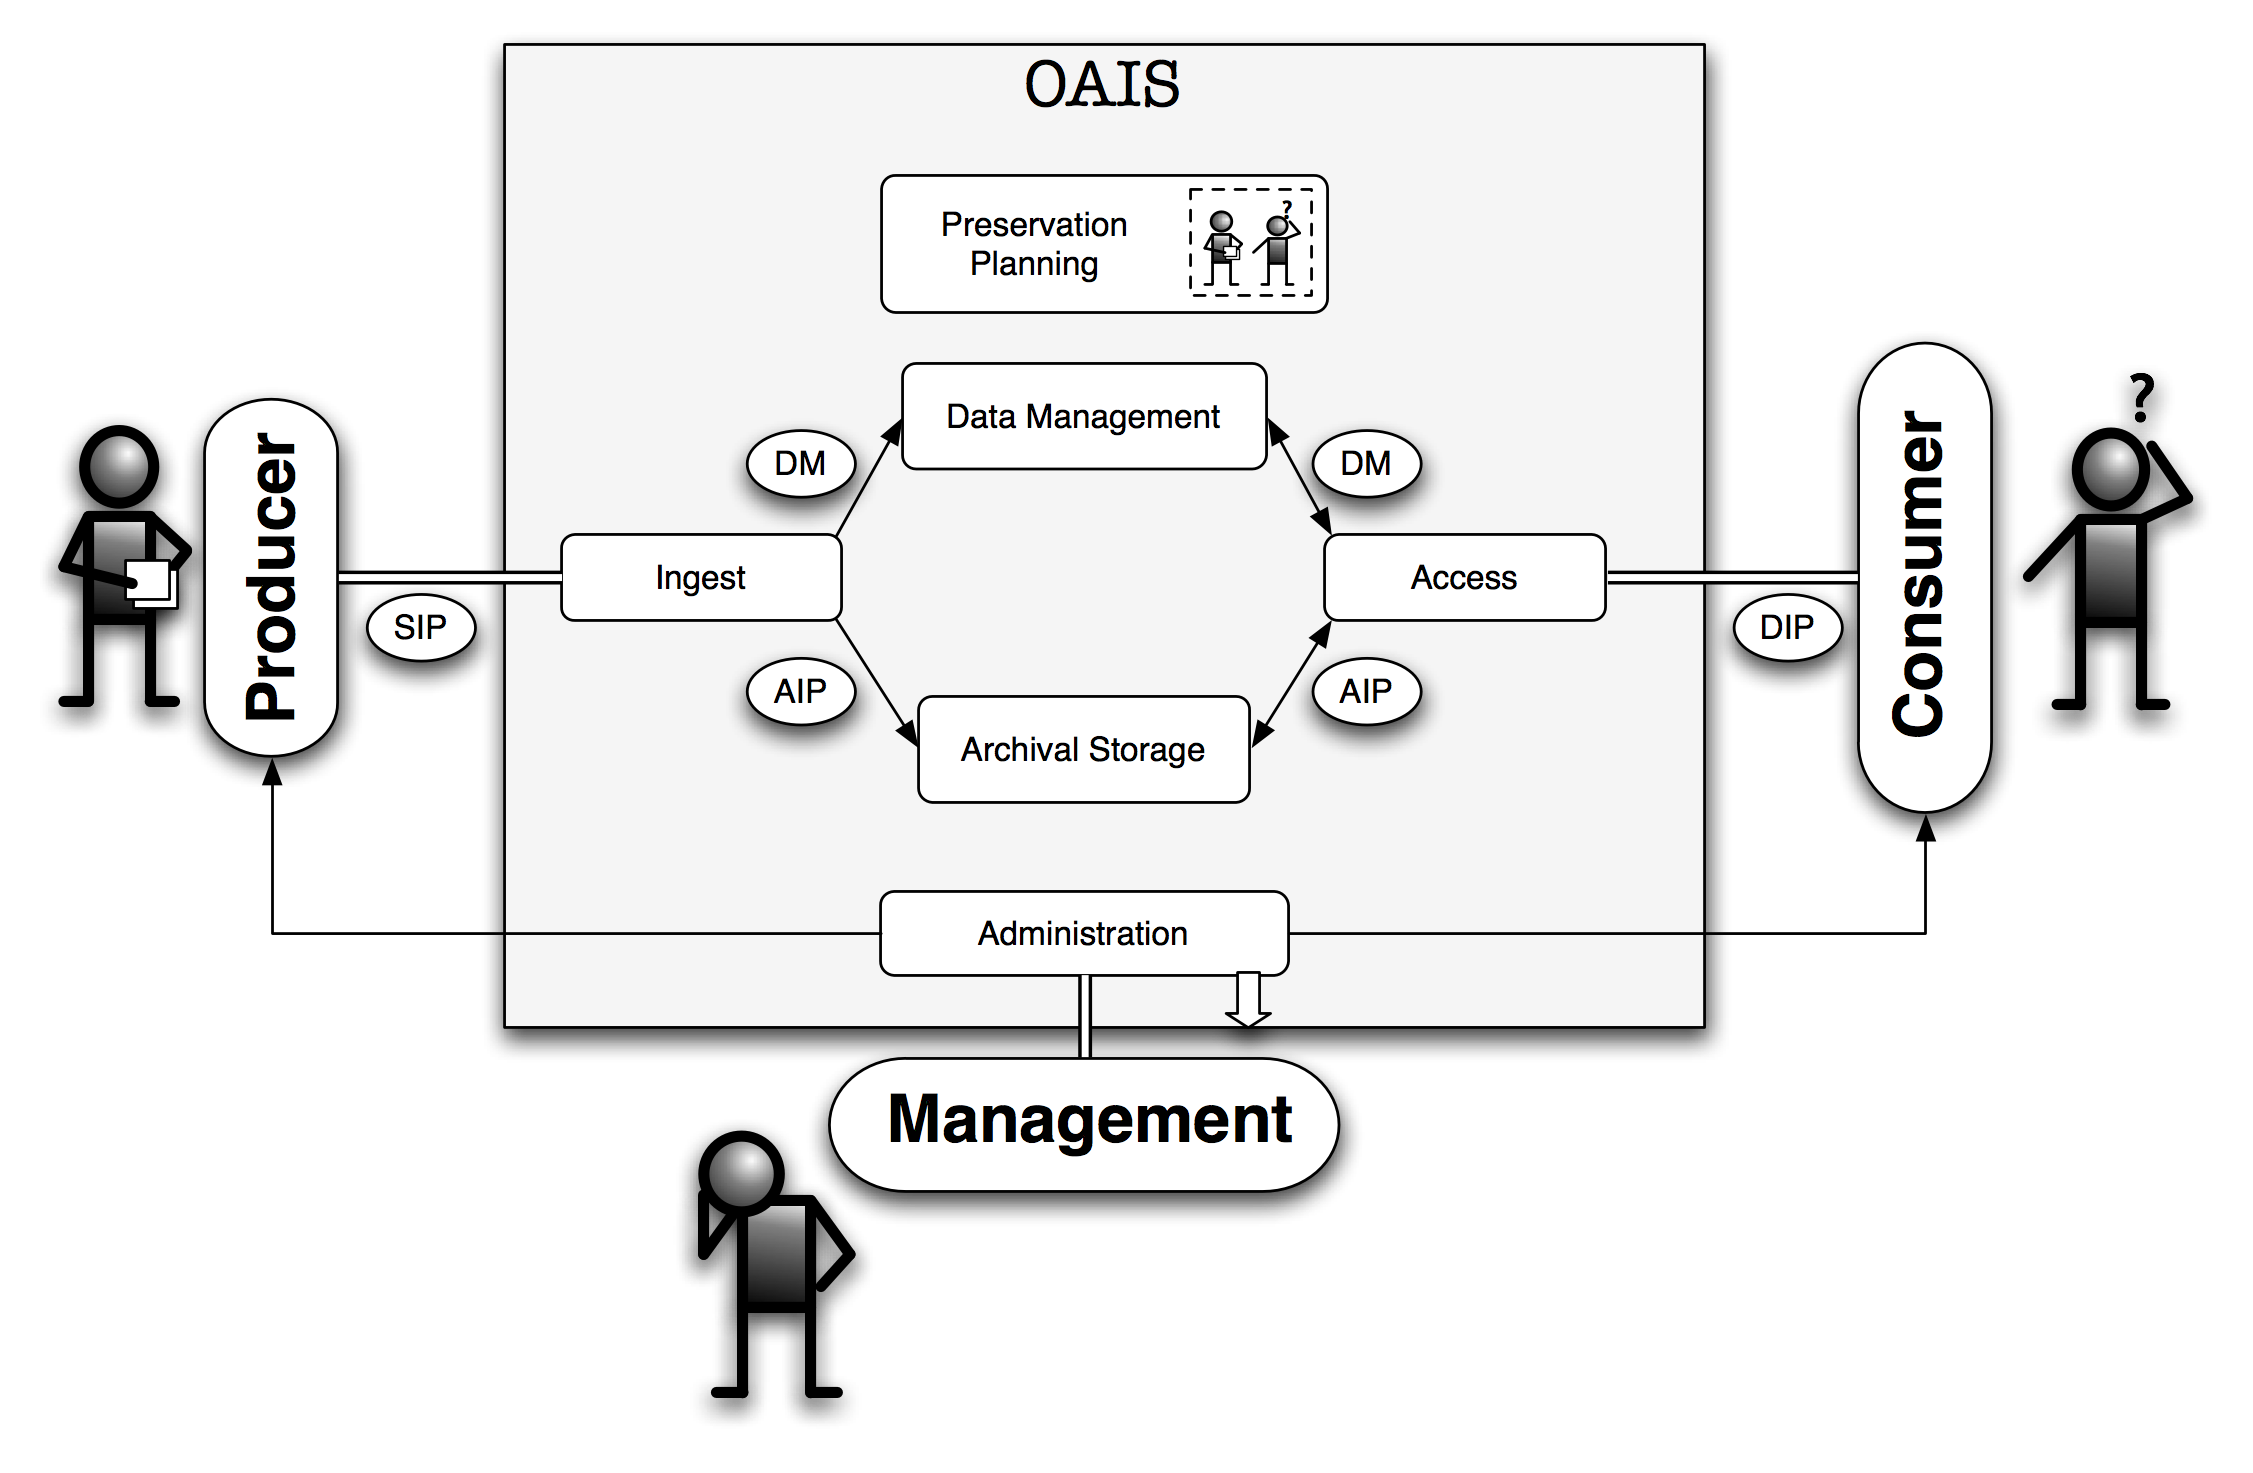
\includegraphics[width=1\textwidth,center]{images/arquitetura/oais}
  \caption{Modelo OAIS}
  \label{fig:oais}
\end{figure}

Como representado na Figura ~\ref{fig:oais}, o sistema irá interagir com três tipos distintos de atores:
\begin{description}[labelindent=1cm]
  \item[Produtores] que serão representados pelos Alunos.
  \item[Administrador] que serão representados pelos Docentes.
  \item[Consumidor] que serão representados por todos os utilizadores do sistema, registados ou não.
\end{description}
E será constituido por três mega processos:
\begin{description}[labelindent=1cm]
  \item[Ingestão] responsável pela receção e depósito de projetos.
  \item[Administração] responsável pela gestão interna do sistema.
  \item[Disseminação] responsável pela disseminação, distribuição e publicação dos objetos arquivados.
\end{description}

\subsection{Fluxo do Sistema}

Com o objetivo de perceber e organizar melhor o fluxo do nosso sistema, construimos um \textbf{Diagrama de Atividade} que de uma forma pouco pormenorizada demonstra sequencialmente as principais ações dos utilizadores do sistema. De notar que este diagrama será importante para perceber a ligação entre os vários utilizadores e as ações dependentes entre estes.

Com o \textbf{Diagrama de Atividade} da Figura ~\ref{fig:diagrama-blocos}, podemos consultar de forma simplificada o fluxo do nosso sistema.

\begin{figure}[H] 
  \centering
  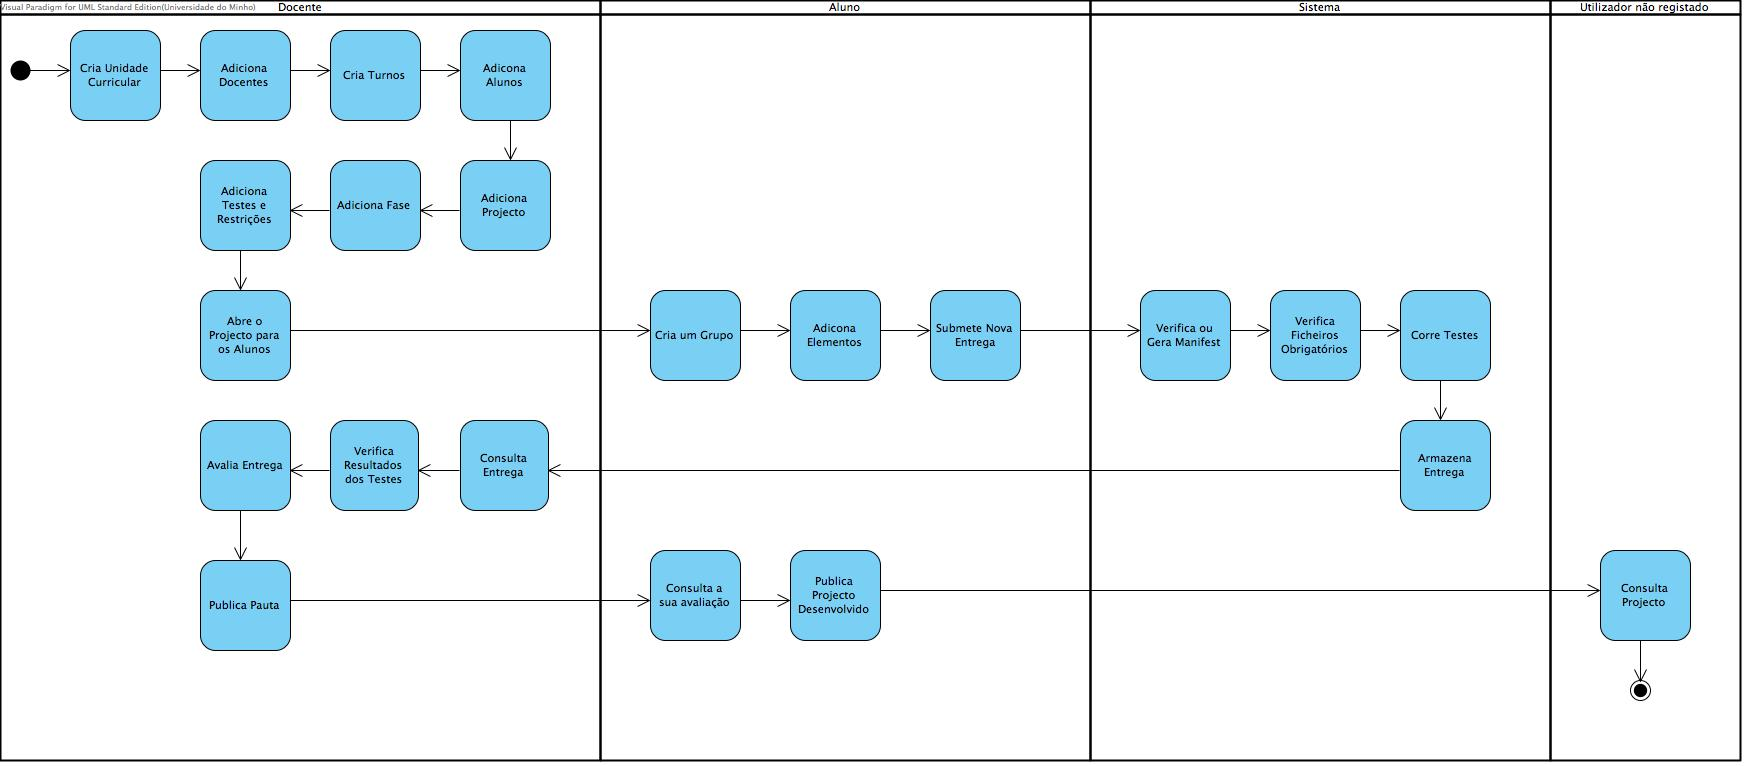
\includegraphics[width=1\textwidth,center]{images/arquitetura/diagrama-blocos}
  \caption{Fluxo do Sistema}
  \label{fig:diagrama-blocos}
\end{figure}

Para a representação do fluxo das funcionalidades mais complexas da aplicação, construiu-se \textbf{Diagramas de Atividade} que permitem representar essas mesmas funcionalidades mais pormenorizadamente.
Estes diagramas para além de ajudarem a perceber melhor o funcionamento do sistema nas tarefas mais relevantes, serão um excelente apoio na implementação do sistema.

Na Figura ~\ref{fig:criacao-projecto} podemos consultar o fluxo de criação de um projeto, desde o acesso ao sistema por parte de um docente, até ao acesso à página do projeto por parte de um aluno.

\begin{figure}[H] 
  \centering
  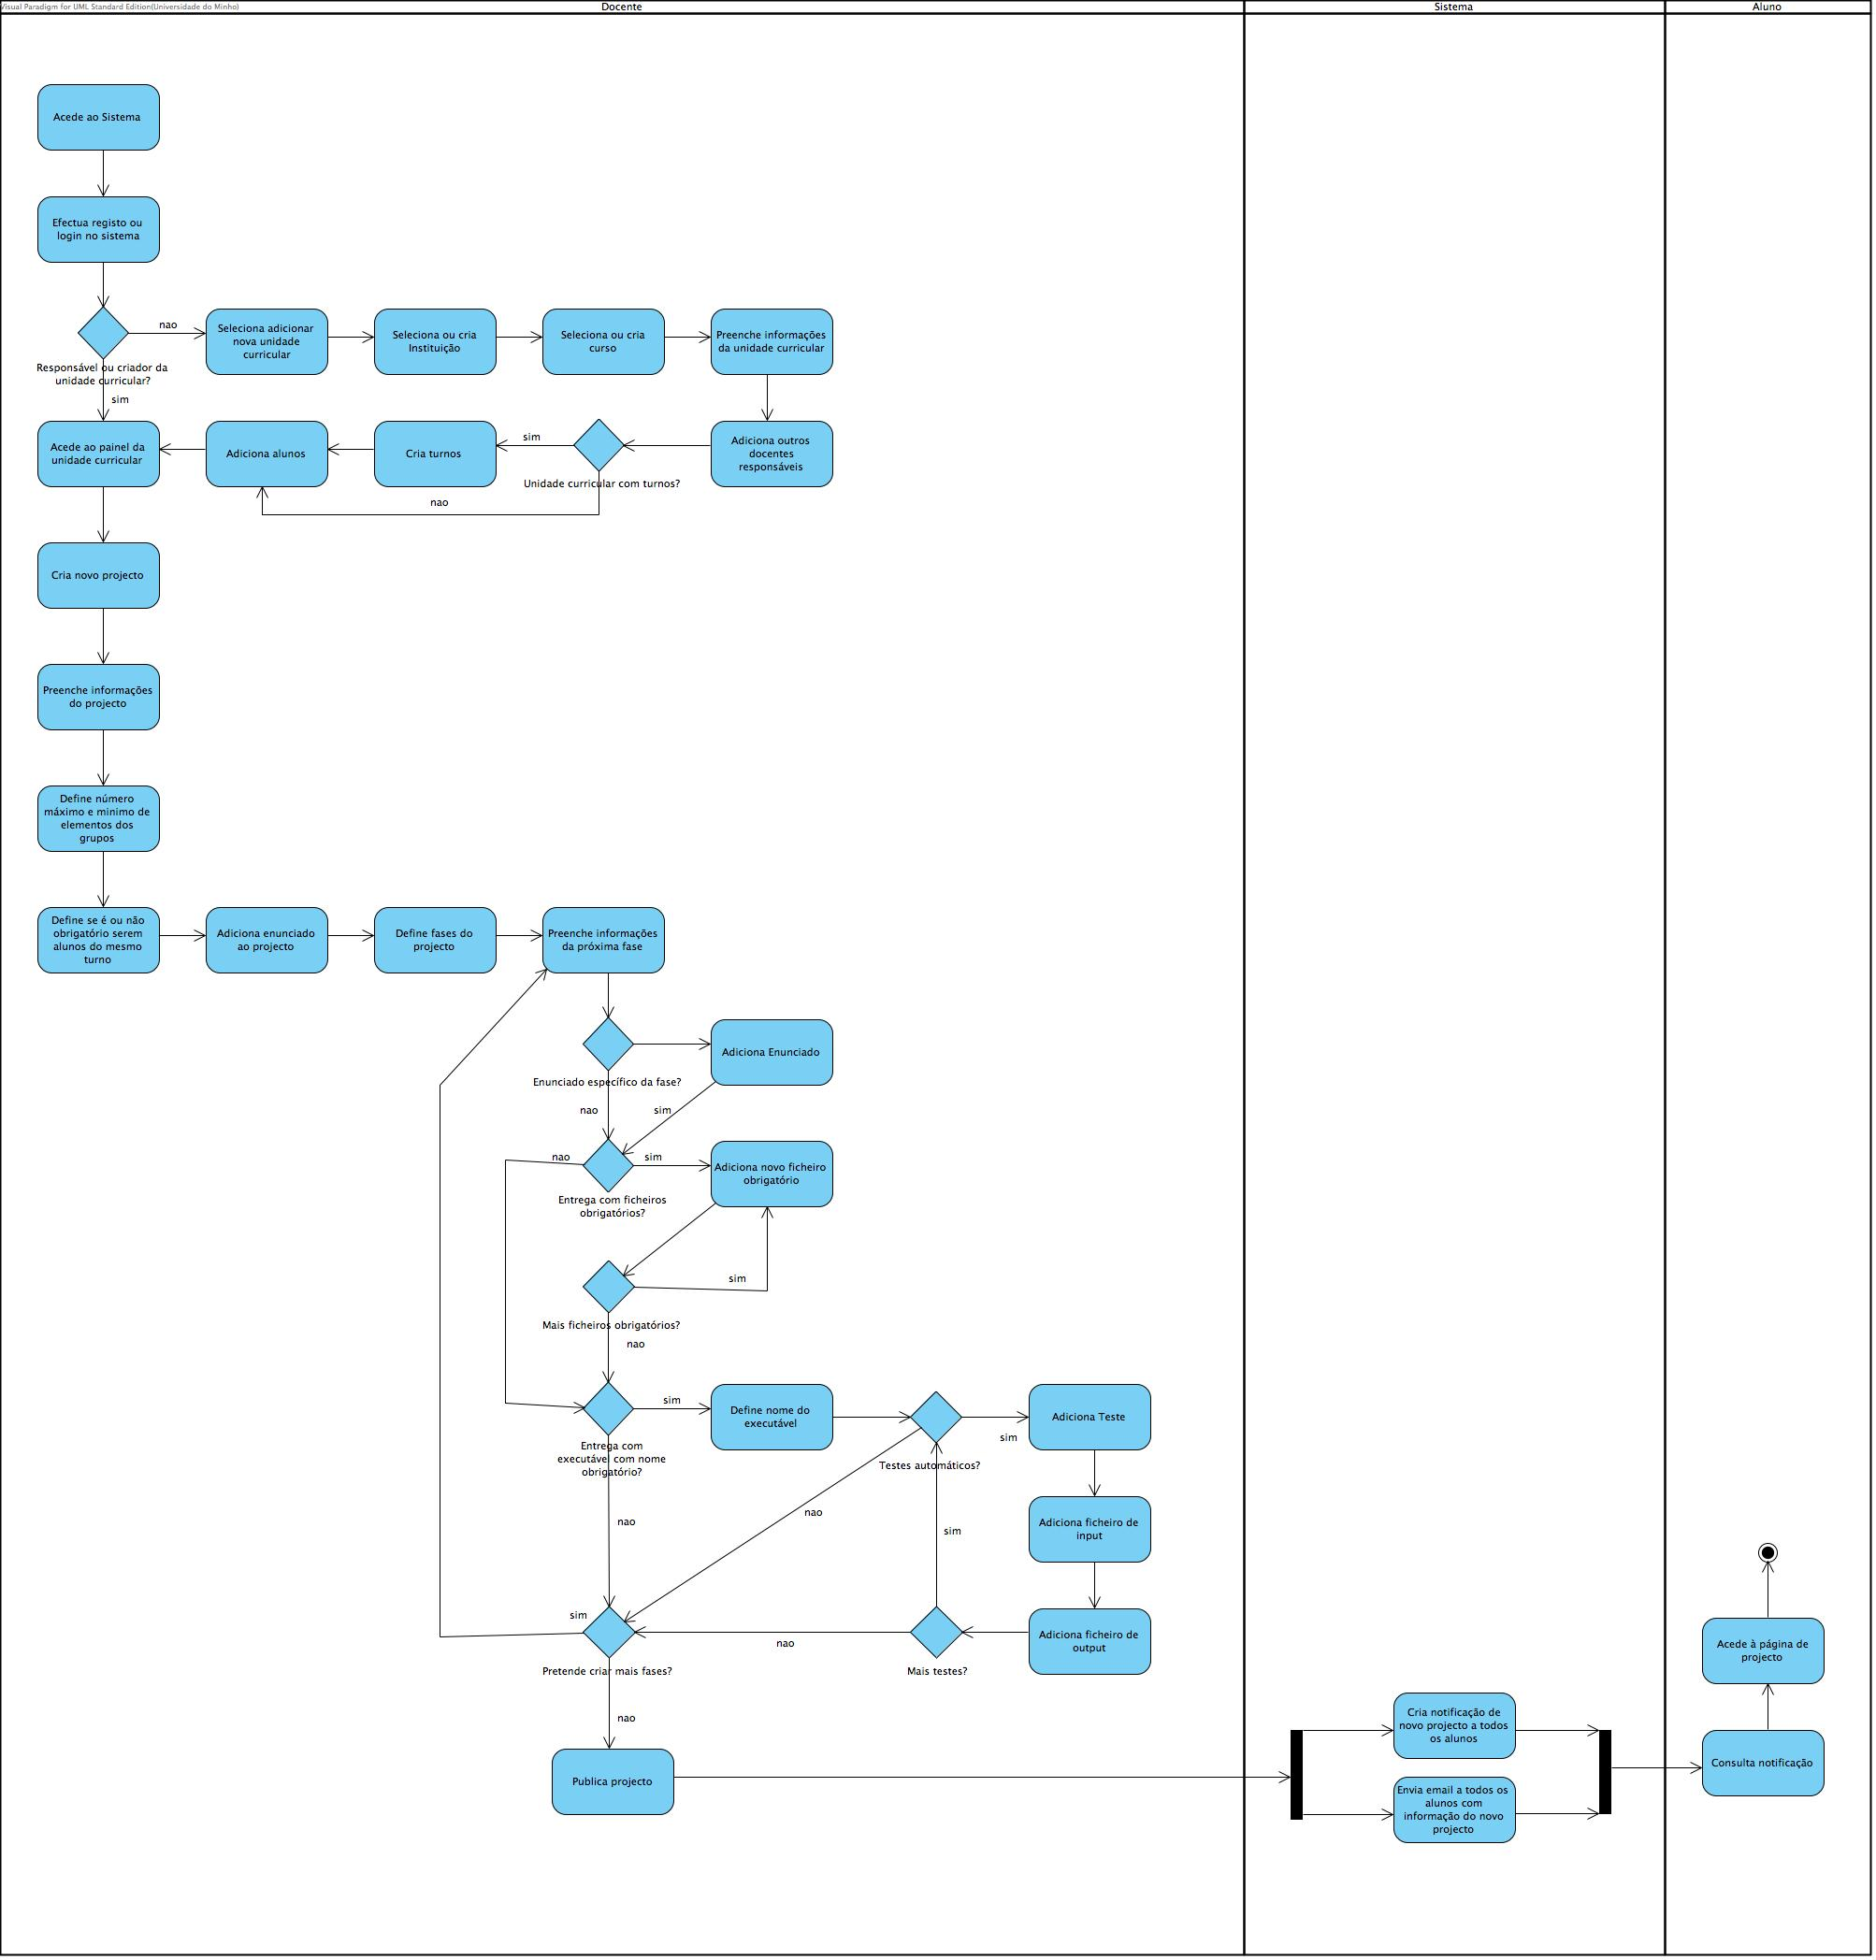
\includegraphics[width=1\textwidth,center]{images/arquitetura/criacao-projecto}
  \caption{Fluxo: Criar Projecto}
  \label{fig:criacao-projecto}
\end{figure}

Na Figura ~\ref{fig:submissao-projecto} podemos consultar o fluxo de submissão de um projeto, desde o acesso à página de um projeto por parte de um utilizador até à consulta das informações da entrega por parte de um docente.

\begin{figure}[H] 
  \centering
  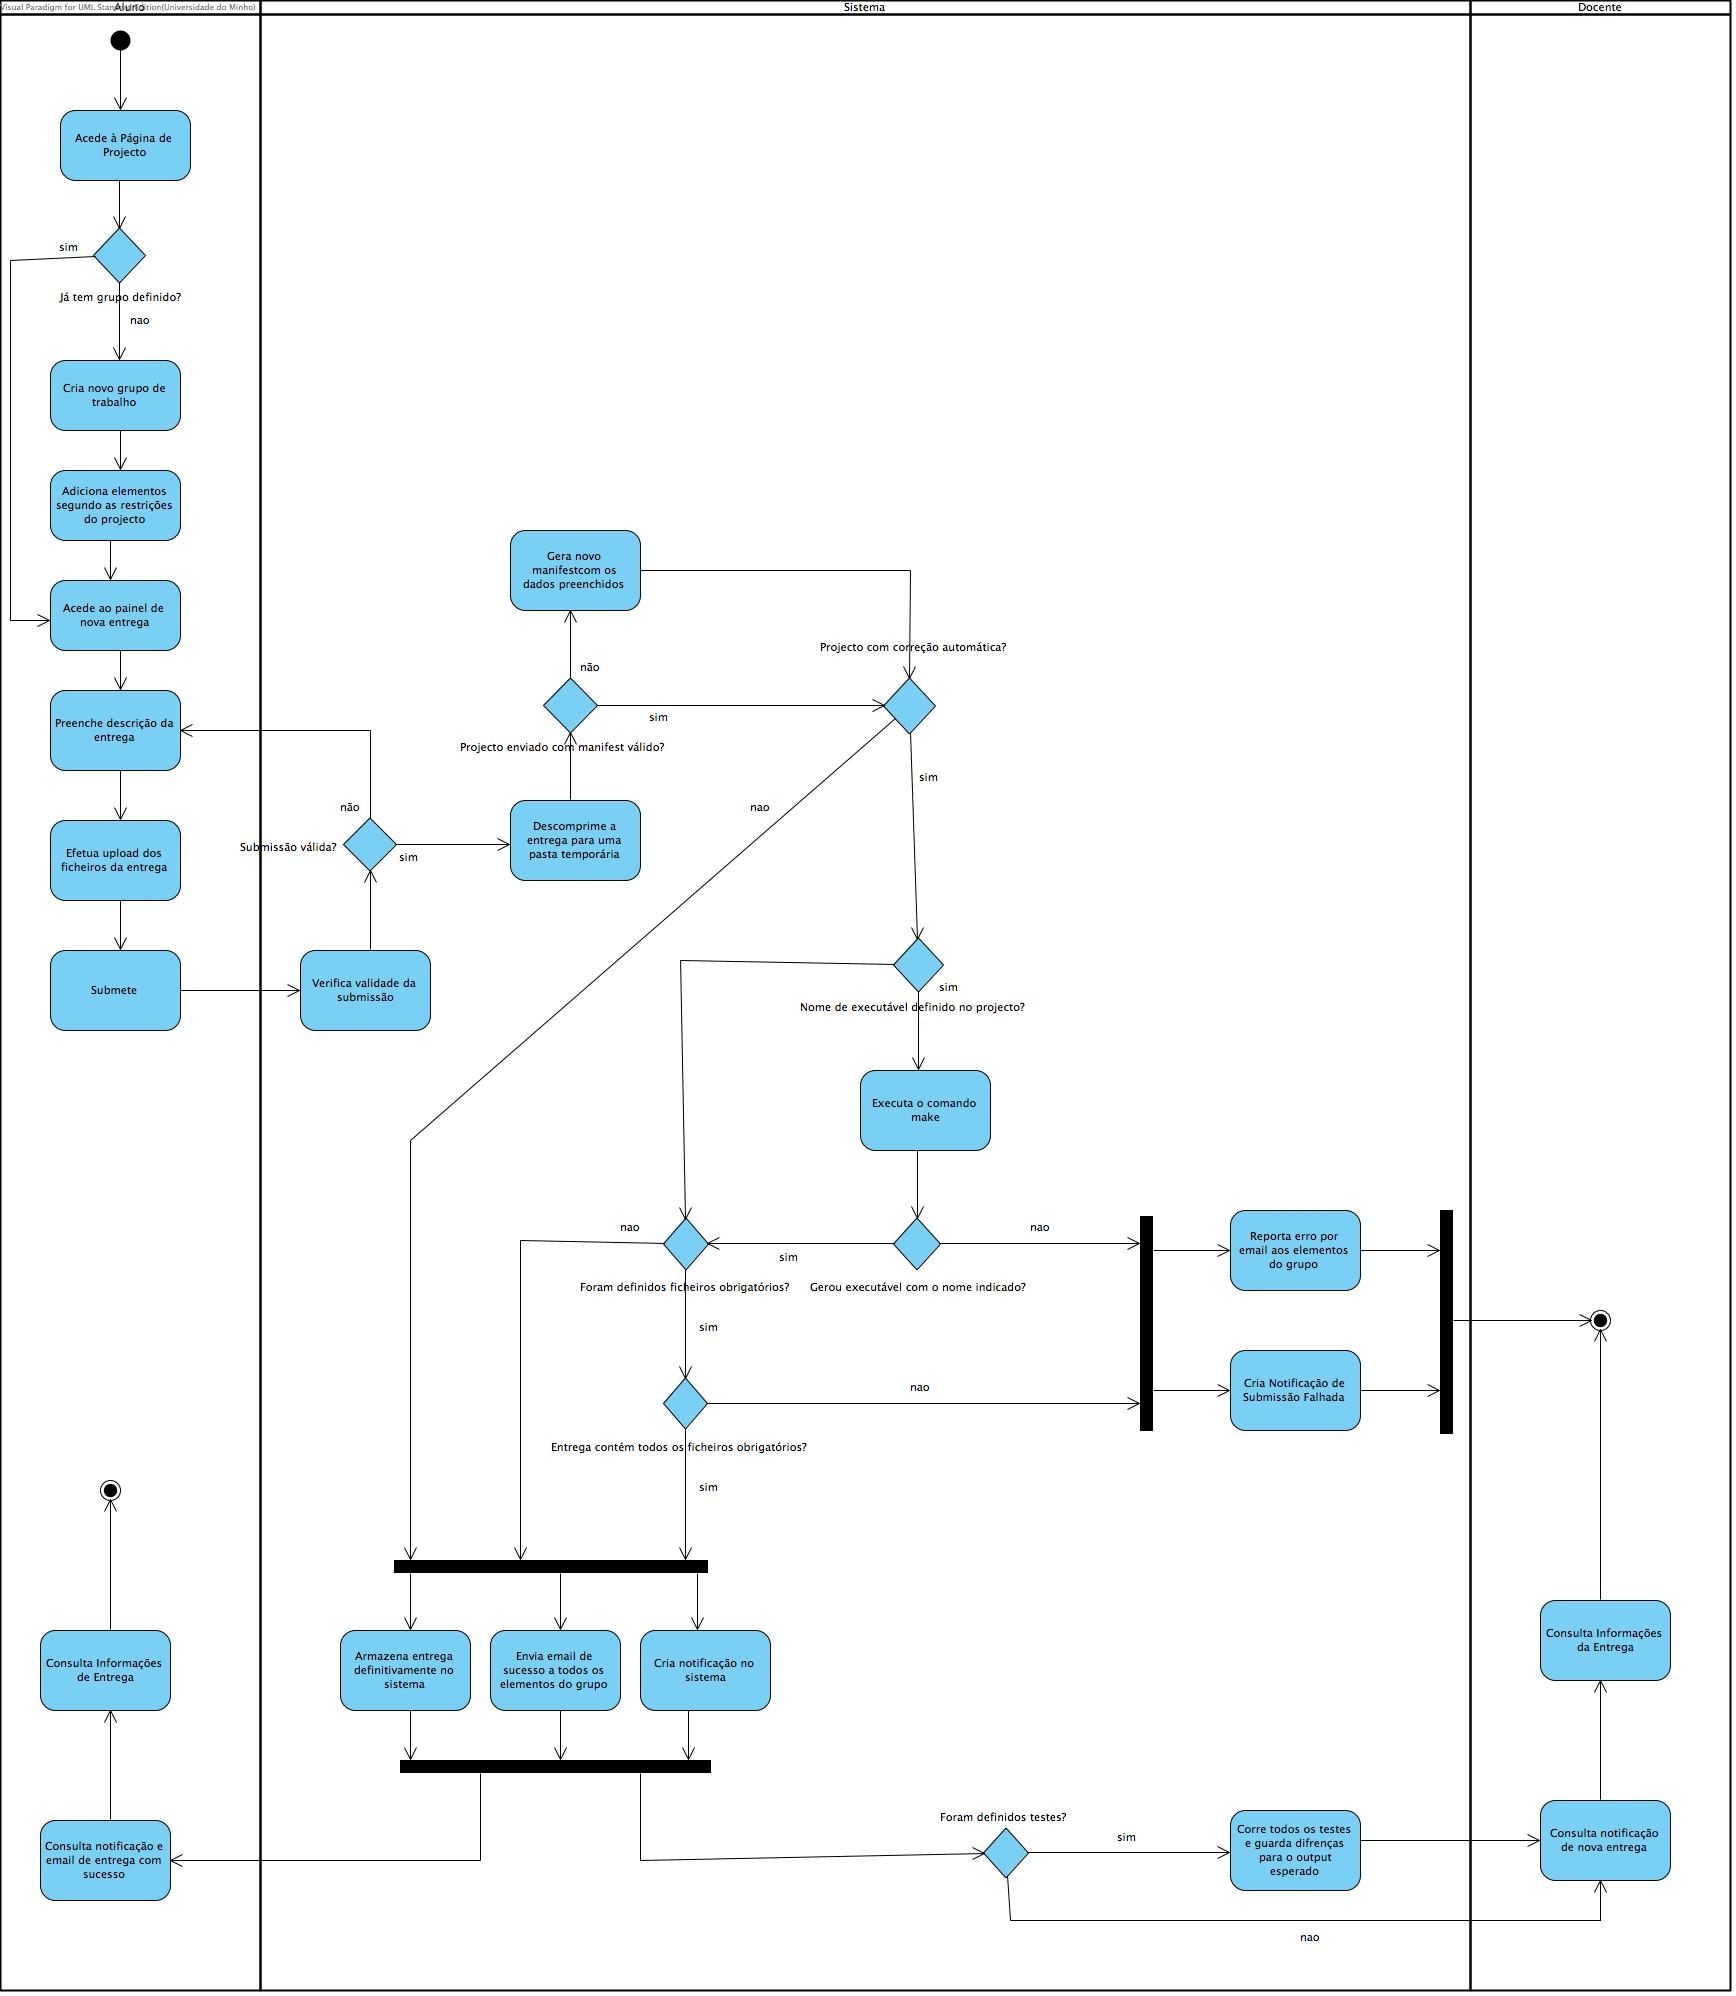
\includegraphics[width=1\textwidth,center]{images/arquitetura/submissao-projecto}
  \caption{Fluxo: Submeter Projeto}
  \label{fig:submissao-projecto}
\end{figure}

\newpage

\section{Modelo de dados}

Uma das componentes importantes do desenho de um sistema de informação, passa por criar um modelo que explique as características de funcionamento e comportamento do \textit{software} a ser desenvolvido. A modulação para além de ajudar na compreensão do sistema, evita erros de programação, de projeto e de funcionamento.

\subsection{Modelo de Domínio}

Um dos primeiros passos na planificação do sistema passou pela definição do \textbf{Modelo de Domínio}.
Pode-se classificar como domínio do sistema, o conjunto de características que descrevem a família de problemas que a aplicação pretende solucionar.

Pode-se consultar na Figura ~\ref{fig:modelo-dominio} os termos do sistema e as relações existentes entre esses termos.

\begin{figure}[H]
  \centering
  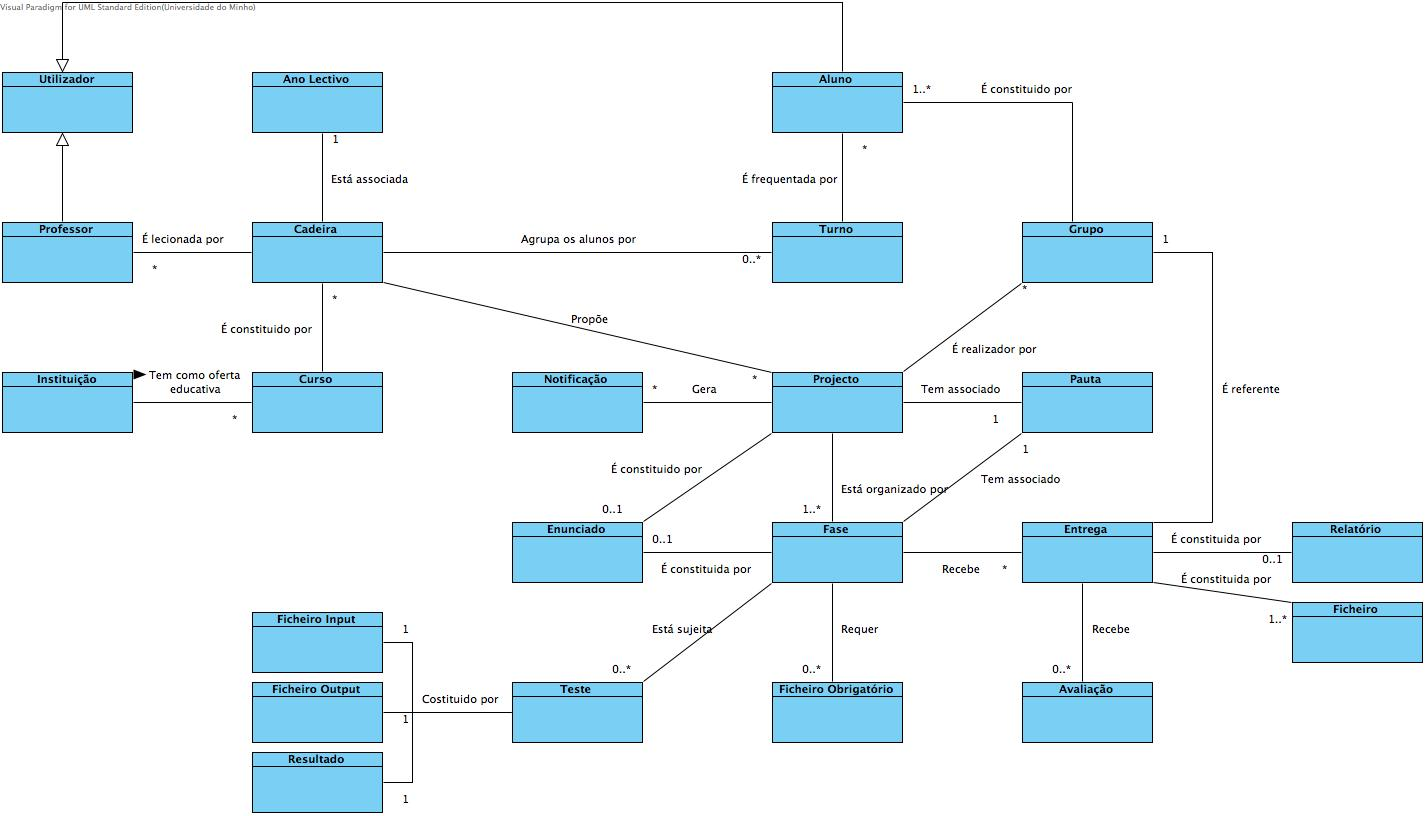
\includegraphics[width=1\textwidth,center]{images/modelo_dados/modelo-dominio}
  \caption{Modelo de domínio}
  \label{fig:modelo-dominio}
\end{figure}

\subsection{Diagrama de Classes}

Para representar a estrutura e relações das classes que servirão de modelo para os objetos do sistema, utilizaremos um \textbf{Diagrama de Classes}. Os diagramas de Classes são extremamente úteis para o desenvolvimento de sistemas, pois definem todas as classes que irão constituir o sistema e são uma excelente base para outras fases de planeamento e para o desenvolvimento.

Este tipo de diagramas permitem verificar como cada classe se relaciona com as outras, tendo como objetivo, a satisfação dos requisitos funcionais definidos para o sistema em estudo.

Na Figura ~\ref{fig:diagrama-classes} podem-se ver representadas todas as classes e as suas relações que servirão como modelo para os objetos do sistema.

\begin{figure}[H]
  \centering
  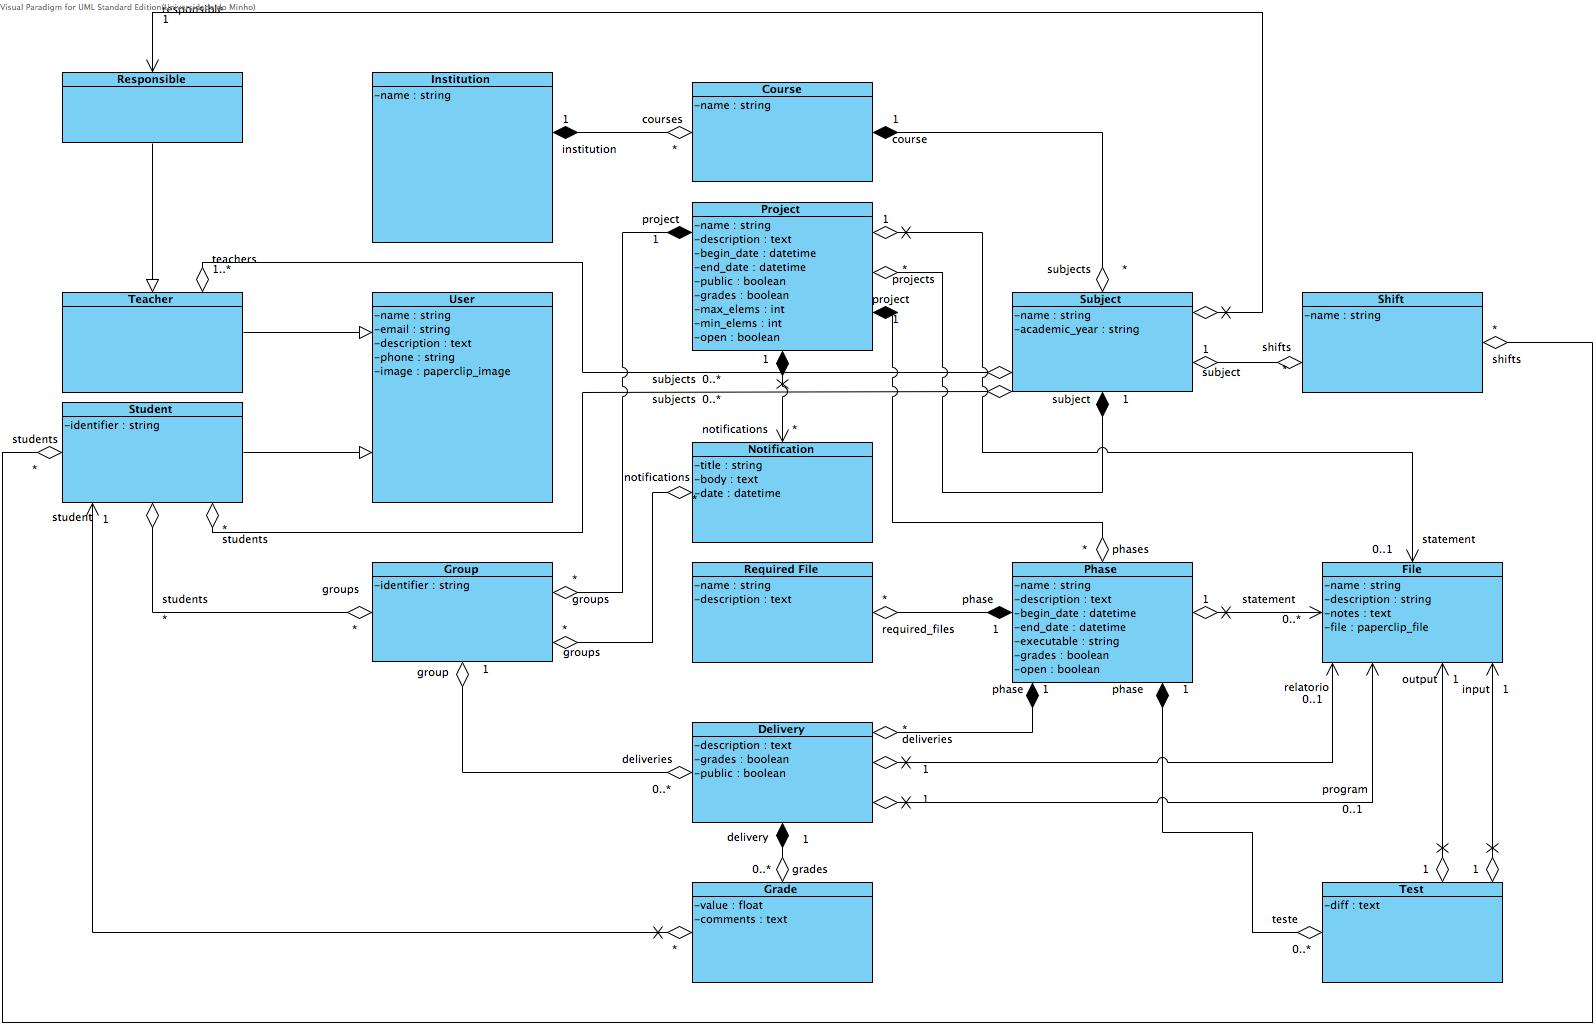
\includegraphics[width=1\textwidth,center]{images/modelo_dados/diagrama-classes}
  \caption{Diagrama de Classes}
  \label{fig:diagrama-classes}
\end{figure}

\subsection{Gramática Independente de Contexto}

Alternativamente ao Diagrama de Classes, definiu-se o sistema numa gramática independente de contexto na forma \textbf{Extended Backus-Naur (EBNF)}, representada de seguida:

\begin{spverbatim}
Institution : Course+ name=STRING
            ;

Course : Subject+ name=STRING
       ;

Subject : name=STRING academic_year=STRING Responsible Shift+ Teacher+ Student+ Project+
        ;

Project : name=STRING description=TEXT begin_date=DATETIME end_date=DATETIME public=BOOLEAN grades=BOOLEAN max_elems=INT min_elems=INT open=BOOLEAN Group+ Notification+ Phase+ statement=Document?
        ;

Notification : title=STRING body=TEXT date=DATETIME Group+
             ;

Shift : name=STRING Subject Student*
      ;

Phase : name=STRING description=TEXT begin_date=DATETIME end_date=DATETIME executable=STRING grades=BOOLEAN open=BOOLEAN Document* statement=Document? Required_Document+ Delivery+ Test*
      ;

Document : name=STRING description=STRING notes=TEXT file=PAPERCLIP_FILE
     ;

Test : diff=TEXT input=Document output=Document
     ;

Required_Document : name=STRING description=TEXT
              ;

Delivery : description=TEXT evaluated=BOOLEAN public=BOOLEAN Grade* Group
         ;

Grade : value=FLOAT comments=TEXT Student
      ;

Group : identifier=STRING Notification+ Delivery* Student+
      ;

Student : User identifier=STRING Shift+ Group+ Subject+
        ;

Teacher : User Subject+
        ;

User : name=STRING email=STRING description=TEXT phone=STRING image=PAPERCLIP_FILE
     ;

Responsible : Teacher
            ;
\end{spverbatim}


\newpage

\section{Repositório de informação}

Para a representação do repositório de informação do sistema, utilizar-se-á um \textbf{Diagrama entidade relacionamento}, que descreve o modelo de dados de um sistema com alto nível de abstração. 

Na Figura ~\ref{fig:der} pode-se consultar todas as tabelas que constituirão o sistema, assim como os seus atributos. De notar que os tipos especificados para os atributos podem não retratar corretamente os tipos que serão utilizados. Como se irá utilizar a \textit{framework} Ruby on Rails para desenvolvimento, esta permite uma maior abstração em relação aos tipos dos atributos da base de dados. Assim sendo os tipos serão definidos segundo o Diagrama de Classes apresentado anteriormente e a \textit{framework} fará a conversão automática conforme a base de dados que estivermos a utilizar.

\begin{figure}[H] 
  \centering
  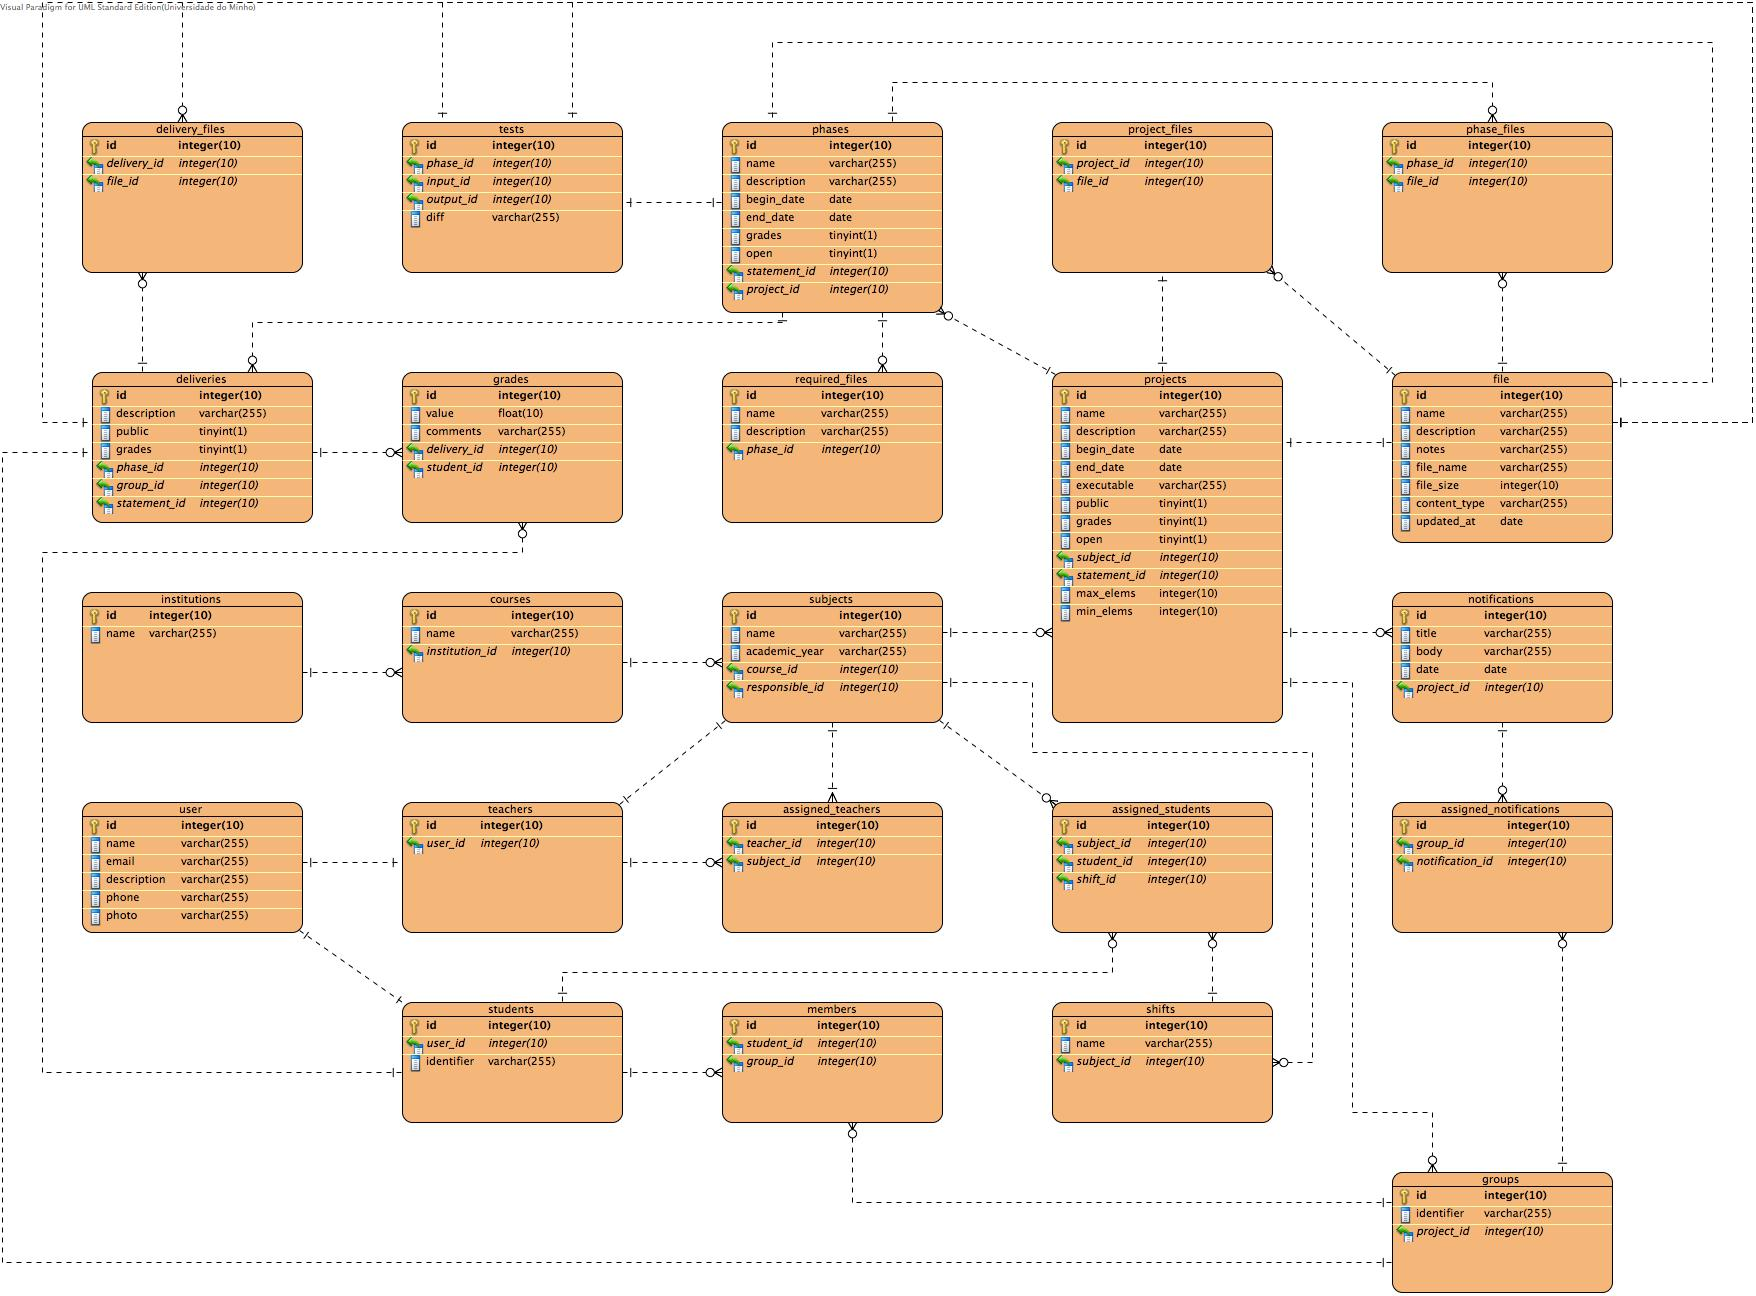
\includegraphics[width=1\textwidth,center]{images/repositorio_informacao/der}
  \caption{Diagrama Entidade Relacionamento}
  \label{fig:der}
\end{figure}

De notar que será utilizado \textbf{SQLite} em ambientes de desenvolvimento e testes, e \textbf{PostgreSQL} para ambientes de produção.

\newpage

\section{Funcionalidades do sistema}

No que diz respeito às funcionalidades do sistema é necessário ter em conta a definição dos seus 
utilizadores e quais as objetivos que a aplicação se propõe a resolver.
Nesse sentido foram definidos três tipos de utilizadores cada um com um conjunto concreto de 
funcionalidades que lhes são fornecidas.
De forma a conseguir fazer este tipo de especificação foram idealizados os seguinte tipos de utilizadores
que interagirão com o sistema, sendo eles: utilizador não registado e utilizador registado na forma de 
docente e aluno.

\begin{figure}[H] 
   \centering
   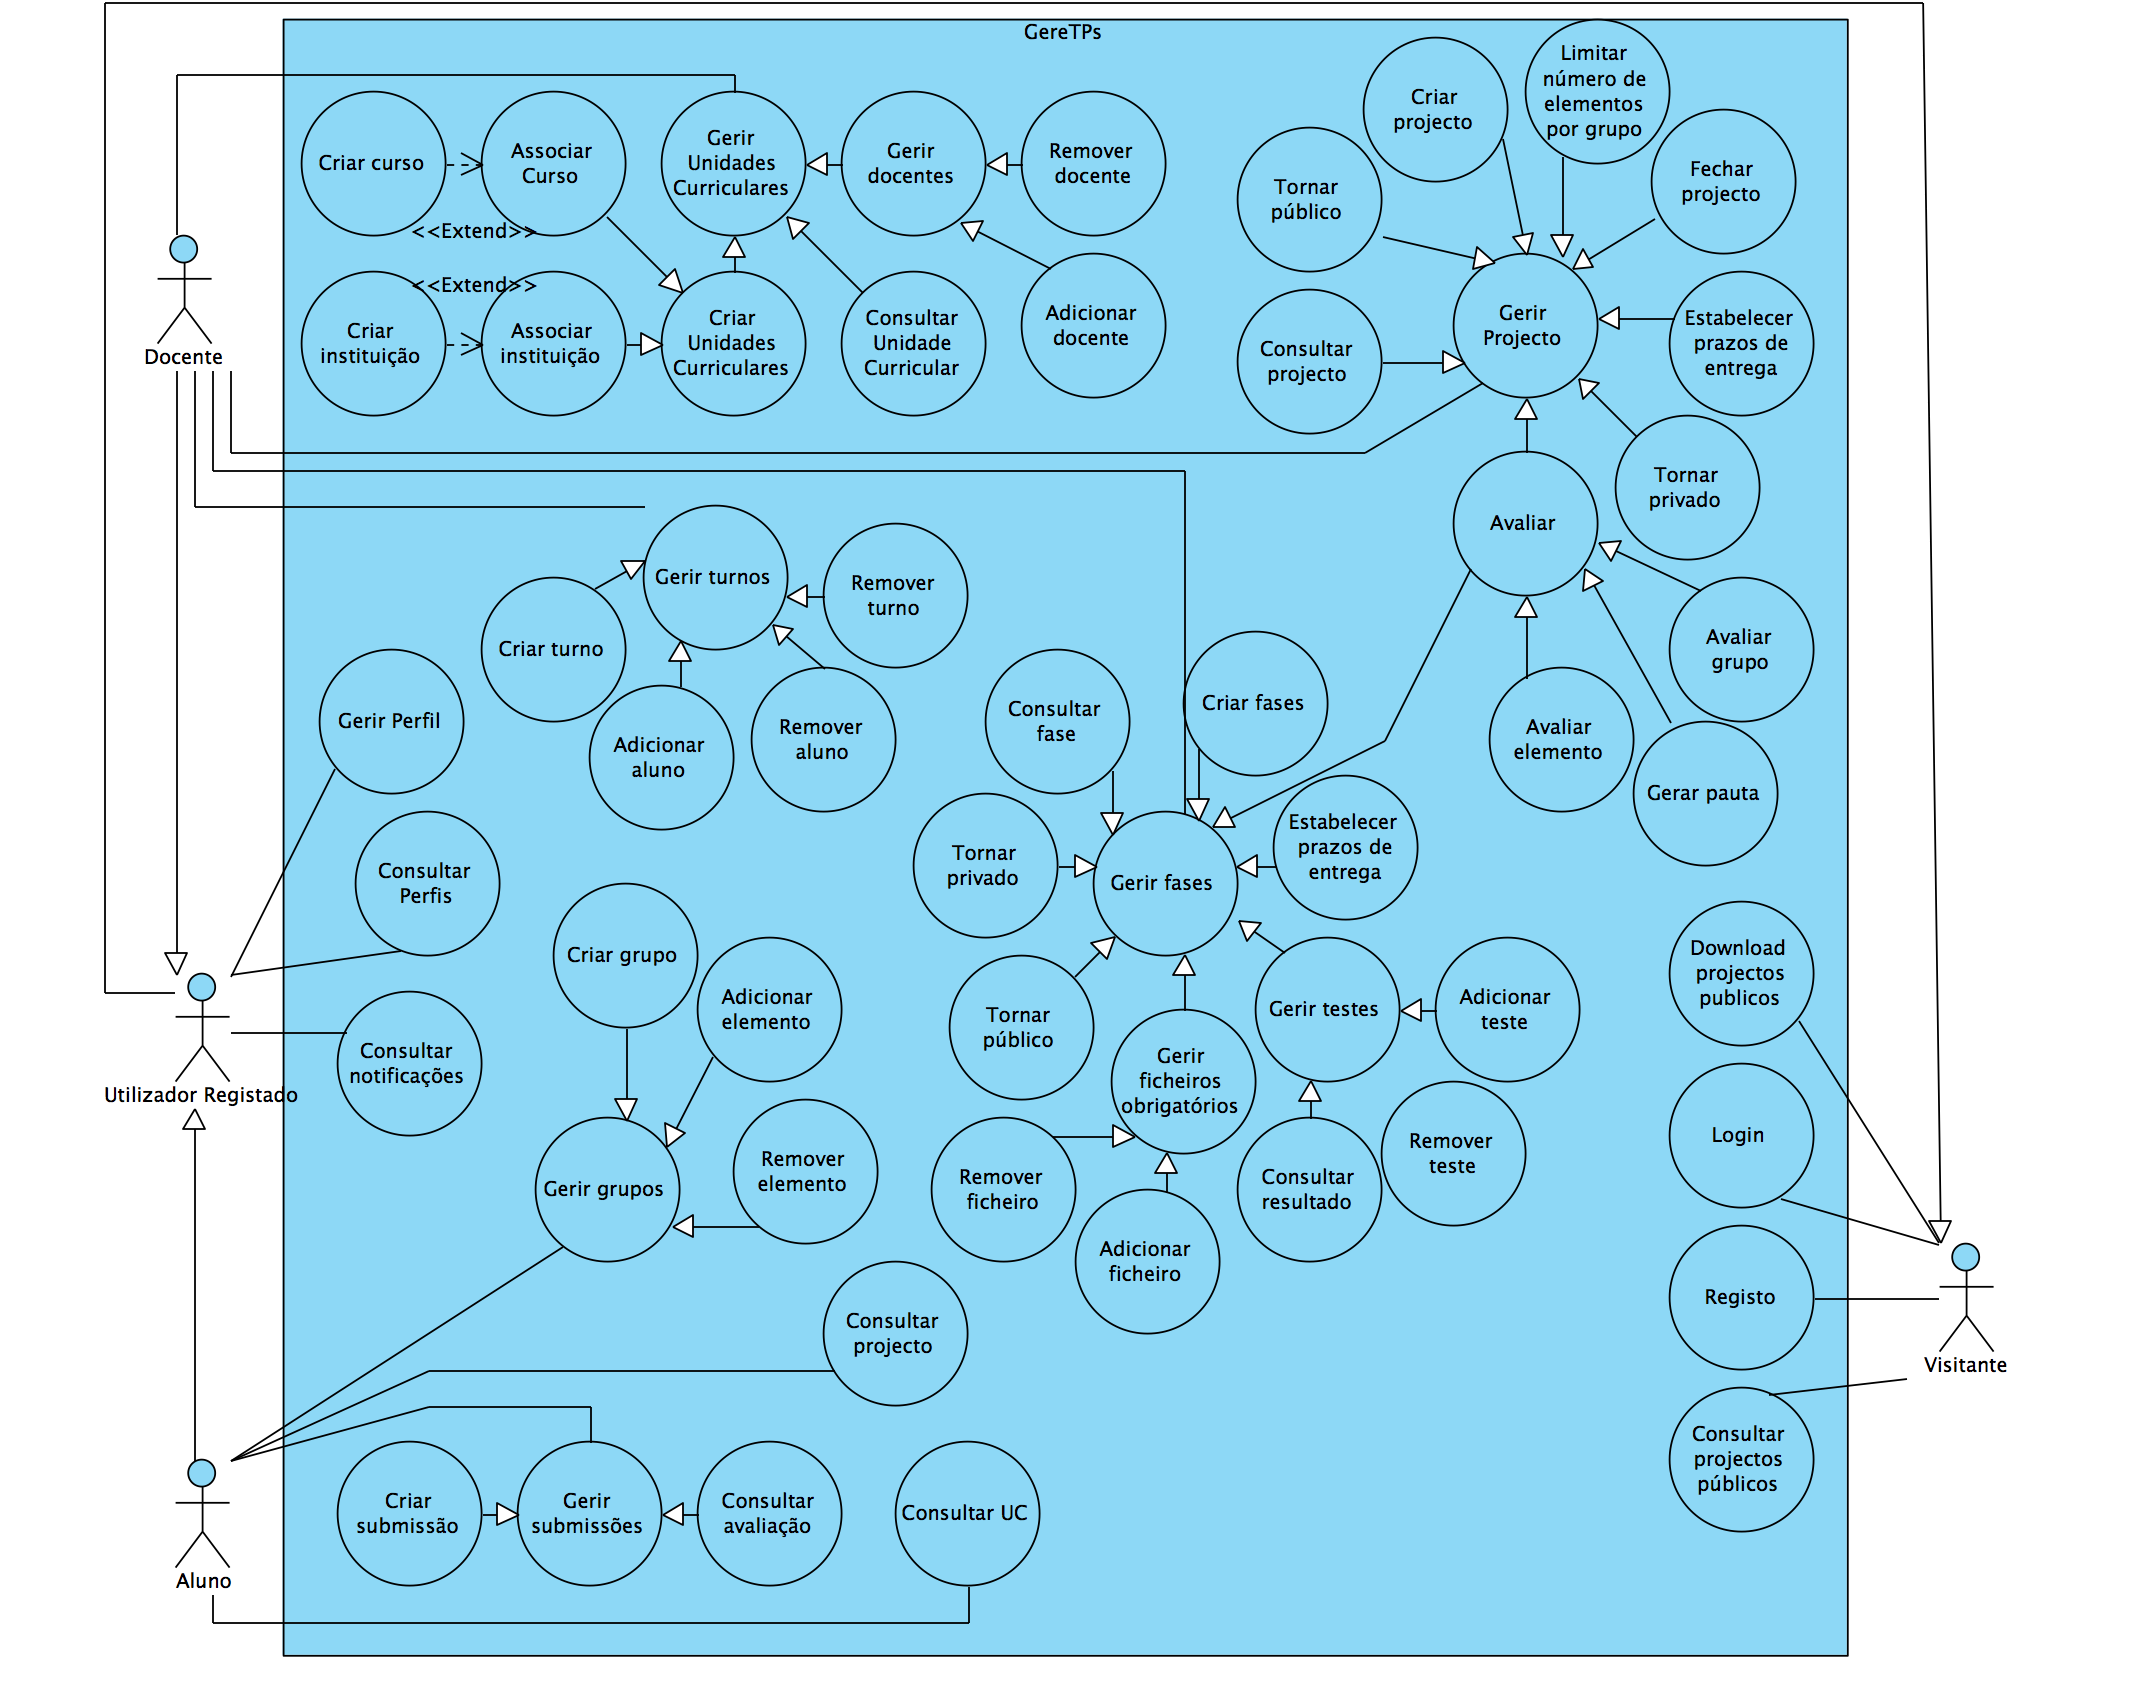
\includegraphics[width=1\textwidth]{images/funcionalidades/usecases.png}
    \caption{Diagrama com casos de uso dos utilizadores do sistema}
    \label{fig: usecases}
 \end{figure}

\subsection{Utilizadores não registados}

Como é possível ver no diagrama de Casos de uso representado na Figura \ref{fig: usecases}, no caso 
dos Utilizadores não registados, representados no diagrama pelo ator Visitante, são disponibilizadas
funcionalidades de registo, entrada no sistema, consulta e \textit{download} de projetos públicos.

Assim sendo é permitido a este tipo de utilizadores registarem-se na aplicação, providenciando informações
pessoais e criando então uma conta persistente com os seus dados, definindo-se a si próprio como
docente ou aluno. Após o registo é-lhes permitida a entrada no sistema com as credenciais de acesso
definidas aquando do registo prévio. Como utilizadores não registados podem também consultar e procurar
todos os projetos disponibilizados por outros utilizadores na aplicação, assim como também lhes é fornecida
a opção de descarregarem os mesmos projetos para o dispositivo de onde acessam.

\subsection{Docentes}

O seguinte tipo de utilizadores descrevem-se como utilizadores registados, sendo-lhes 
disponibilizadas funcionalidades específicas dentro do ambiente da aplicação. Nesse sentido, para 
além de serem uma extensão de Utilizadores não registados após o registo, são-lhes conferidas um
grupo de funcionalidades adicionais que descrevem o comportamento deste tipo de utilizador.

A um docente são disponibilizados quatro grupos de funcionalidades, como é possível observar na Figura
\ref{fig: usecases}. Esses grupos de funcionalidades são a gestão de unidades curriculares, turnos, 
projetos e fases.

No que diz respeito à gestão de unidades curriculares é tornado possível a este tipo 
de utilizador vários tipos de ações sobre as mesmas, nomeadamente, a consulta, a criação e 
remoção, a gestão de docentes, atualização das informações associadas, entre 
outras.

Para além disso, dentro de uma unidade curricular também é possível proceder-se 
à gestão de turnos. Nesse aspeto, é providenciado ao docentes tarefas como consulta, 
criação e remoção de turnos bem como a adição e remoção de alunos desses mesmo 
turnos.

Relativamente à gestão dos projetos de uma unidade curricular são fornecidas 
aos docentes as ferramentas para a consulta, criação e remoção, publicação, 
estabelecimentos de prazos assim como limitações ao número de elementos de um 
grupo, avaliação de um elemento ou grupo e por fim para geração de pautas, de 
todos os projetos associados a uma unidade curricular onde o docente seja 
responsável.

Por fim, a gestão de fases de um projeto é definida por funcionalidades como a 
sua criação e remoção, consulta, tipo de visibilidade, definição de 
obrigatoriedade de ficheiros, definição de testes sobre entregas e estabelecimento de prazos limite 
para submissões.

\subsection{Alunos}

Tal como o tipo de utilizador Docente, o tipo de utilizador Aluno é uma extensão 
de um utilizador não registado após o registo. Este tipo de utilizador é 
definido pelas funcionalidades que lhe são disponibilizadas pelo sistema. Dentro 
destas funcionalidades podemos destacar um conjunto delas, nomeadamente a 
consulta de projetos e unidades curriculares, a gestão de grupos e de submissões de projetos.

No que diz respeito à gestão de grupos é possível um aluno criar um grupo dentro 
de um projeto e adicionar e remover outros alunos como elementos do grupo.

Para além disso também são disponibilizadas ferramentas na aplicação que permite 
aos alunos fazerem submissões ou entregas de projetos dentro de uma unidade 
curricular de onde façam parte de um dos turnos. Para além disso também lhes é 
possível consultar as avaliações dadas pelos docentes às suas submissões assim 
como consultar a unidade curricular e as pautas da mesma.

\newpage

\section{Protótipos para a interface da aplicação}

Um dos processos de desenvolvimento de uma Aplicação Web é a criação de protótipos. Este processo tem como objetivo demonstrar de que forma o utilizador interage com a aplicação e ajuda a tomar decisões antes da implementação da aplicação. Desta forma há um maior entendimento entre o utilizador e a equipa de desenvolvimento e aumenta a usabilidade da aplicação por parte do utilizador, uma vez que são garantidas as seguintes habilidades:

\begin{description}
	\item[Fácil apendizagem] A utilização da aplicação requer pouco treino
	\item[Fácil de memorizar] O utilizador lembra-se de como utilizar a interface depois algum tempo
	\item[Maximizar a produtividade] A realização de uma tarefa é feita de forma rápida e eficiente
	\item[Minimizar a taxa de erros] A aplicação avisa o utlizador, caso existam erros e ajuda na correção dos mesmos
	\item[Maximizar a satisfação] A aplicação transmite confiança e segurança ao utilizador
\end{description}

 \subsection{Primeiros protótipos}

Durante a produção dos primeiros protótipos, teve-se como objetivo identificar de que formas as várias funcionalidades do sistemas iriam estar presentes na aplicação, sem haver preocupações com questões estéticas.Este protótipos são fundamentais, uma vez que demonstrem alguns dos cenários mais complexos e ajuda a compreensão de fluxos ou processos.
Este protótipos foram desenvolvidos usando a aplicação \href{http://balsamiq.com/products/mockups/}{\emph{Balsamiq Mockups}}(Figura ~\ref{fig: balsamiq}).\\

 \begin{figure}[H]
        \centering
        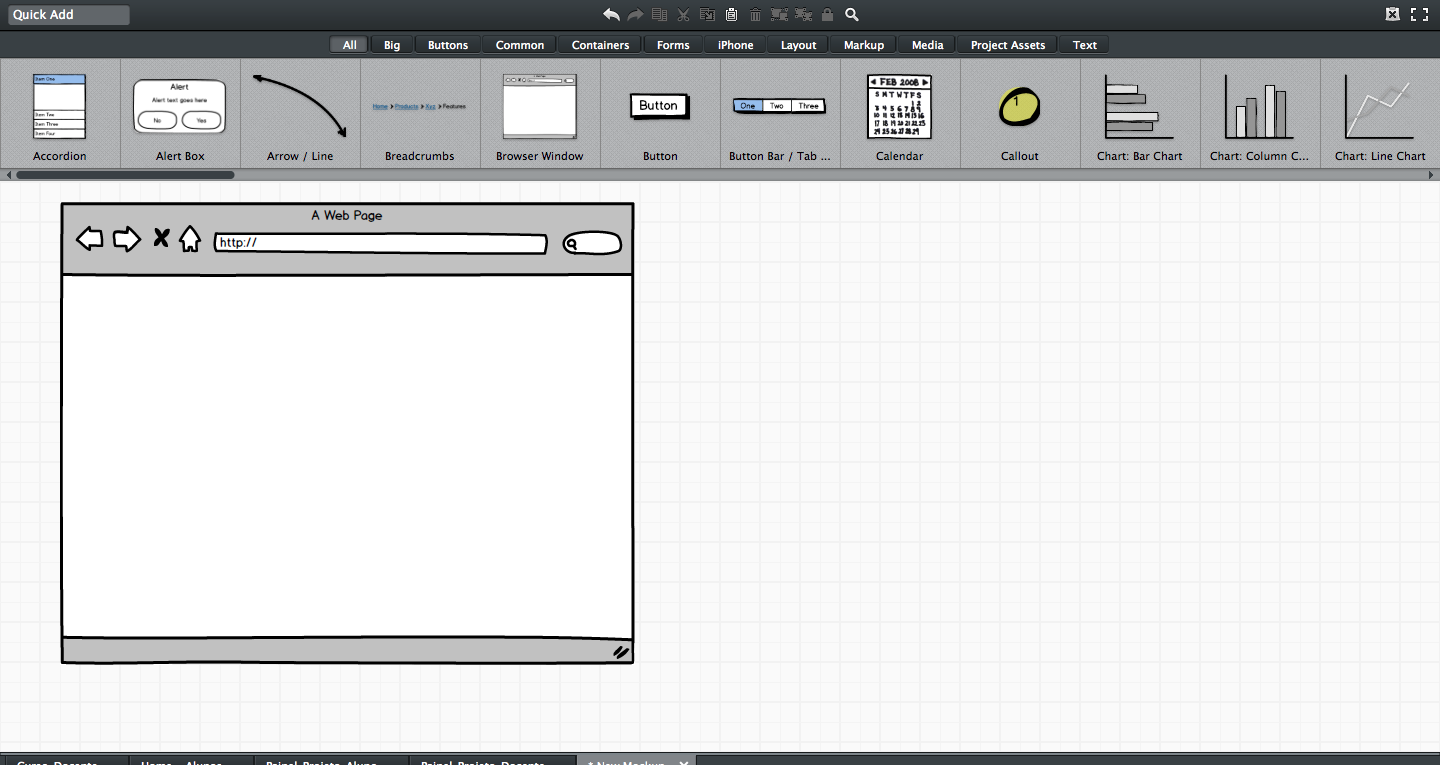
\includegraphics[width=1\textwidth]{images/prototipos/mockups/balsamiq.png}
         \caption{\emph{Balsamiq Mockups}}
         \label{fig: balsamiq}
\end{figure}

Sobre os protótipos desenvolvidos, teve-se como preocupação a simplicidade da página, a quantidade de informação e o tempo de navegação, isto é a quantidade de ações que um utilizador tem que fazer para passar de uma página para outra.\\
Começando pela página inicial (Figura ~\ref{fig: home}) está mostra as várias funcionalidades da aplicação, fazendo a distinção entre alunos e docentes.A partir da página inicial o utilizador pode fazer efetuar registo, login ou procura projetos públicos. \\

\begin{figure}[H]
        \centering
        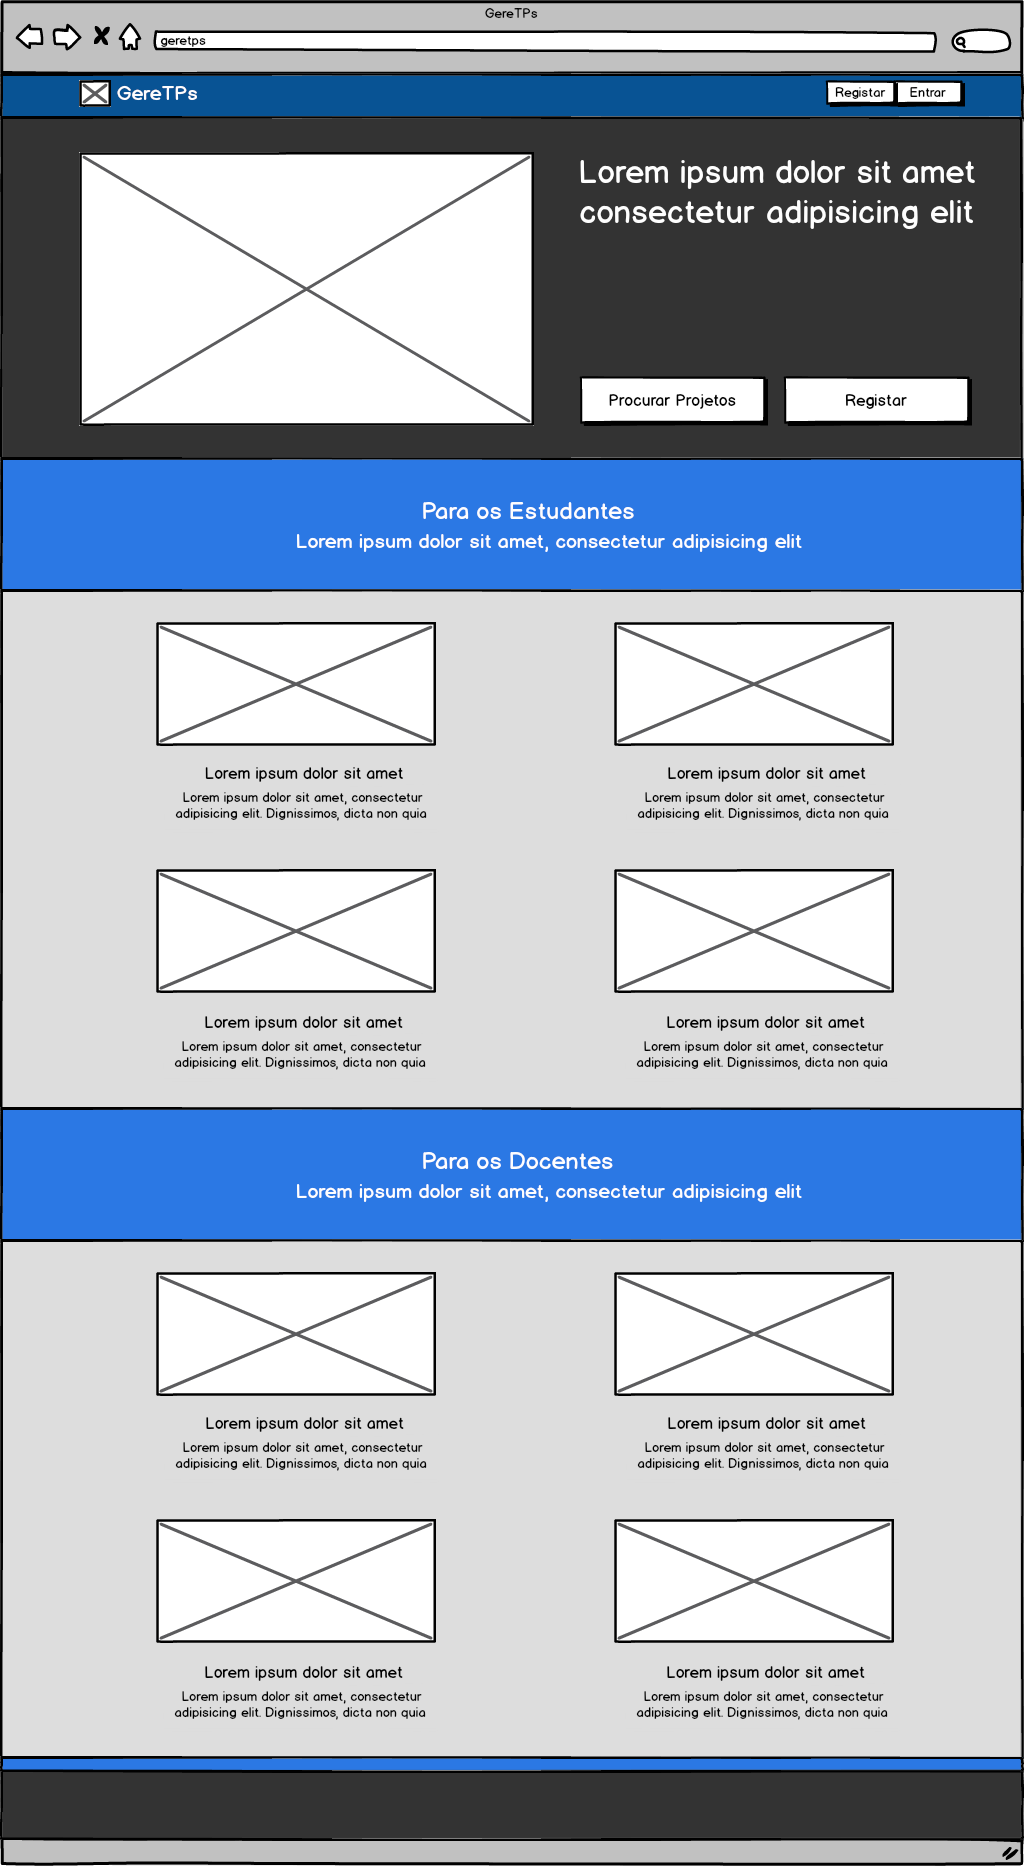
\includegraphics[width=0.73\textwidth]{images/prototipos/mockups/home.png}
         \caption{Página inicial}
         \label{fig: home}
\end{figure}

No painel de uma disciplina(Figura ~\ref{fig: cursodocente}), um docente pode ter acesso aos últimos acontecimentos dentro das disciplina, sabendo quando aconteceram submissões nos projetos desta, assim como alterações da mesma.Também existem informações sobre os projetos criados na disciplina, no qual são apresentadas informações sobre o nome do projeto, número de fases, estado e número de entregas até ao momento. Também é possível adicionar professores de forma direta sem que haja a necessidade de abrir formulários adicionais e fazer gestão de turnos. Caso contrário apenas poderá ver o estado dos turnos e quais são os docentes da disciplina.\\

\begin{figure}[H]
        \centering
        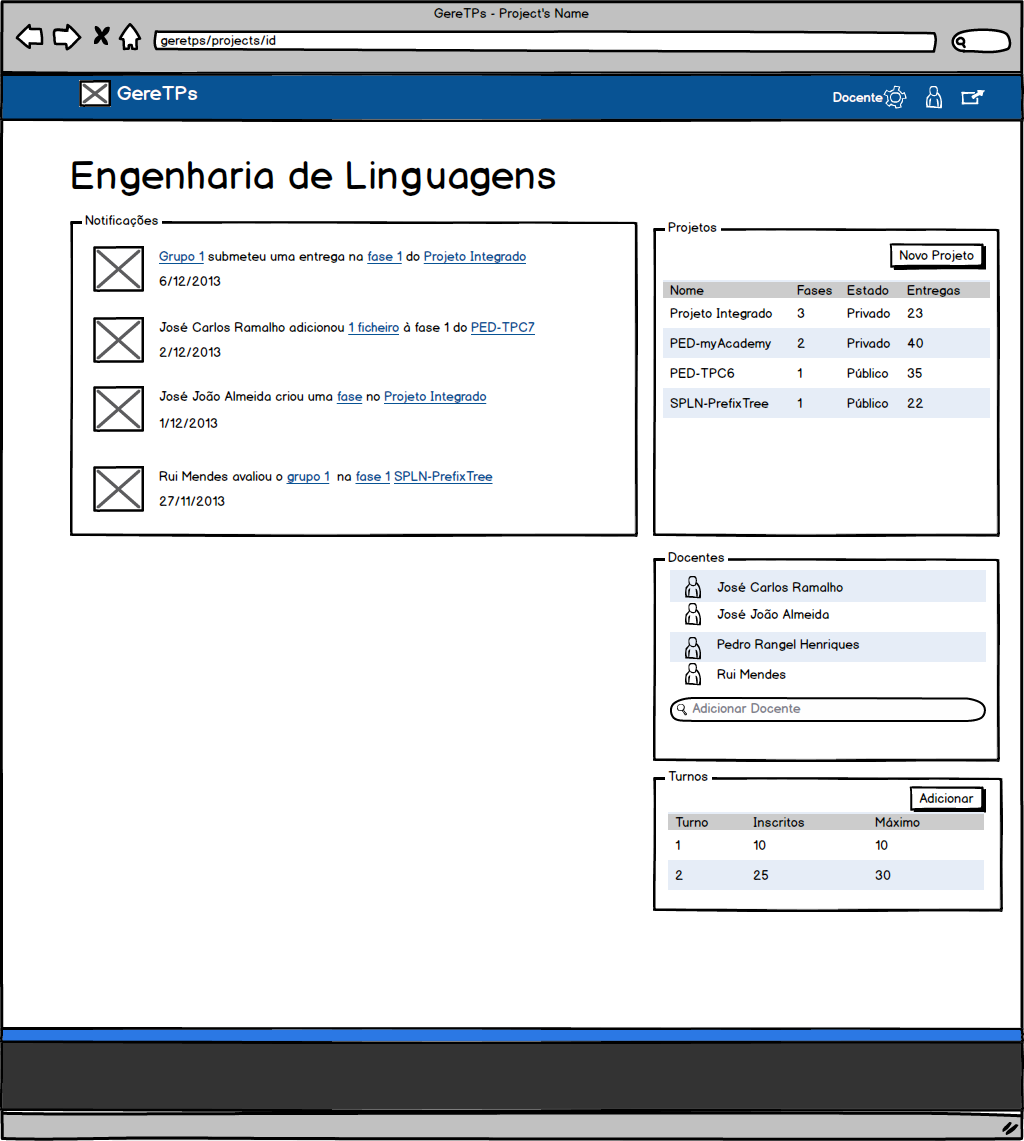
\includegraphics[width=1\textwidth]{images/prototipos/mockups/cursodocente.png}
         \caption{Painel de projeto de um aluno}
         \label{fig: cursodocente}
\end{figure}

Na painel de pesquisa de projetos(Figura ~\ref{fig: projetospublicos}), todos os utilizadores tem acesso aos projetos públicos. Nesta página o utilizador pode filtrar uma pesquisa de forma a que o processo seja mais rápido. Os resultados de uma pesquisa são apresentados sob forma de blocos, desta forma, garante-se um maior aproveitamento do espaço livre da página.\\

\begin{figure}[H]
        \centering
        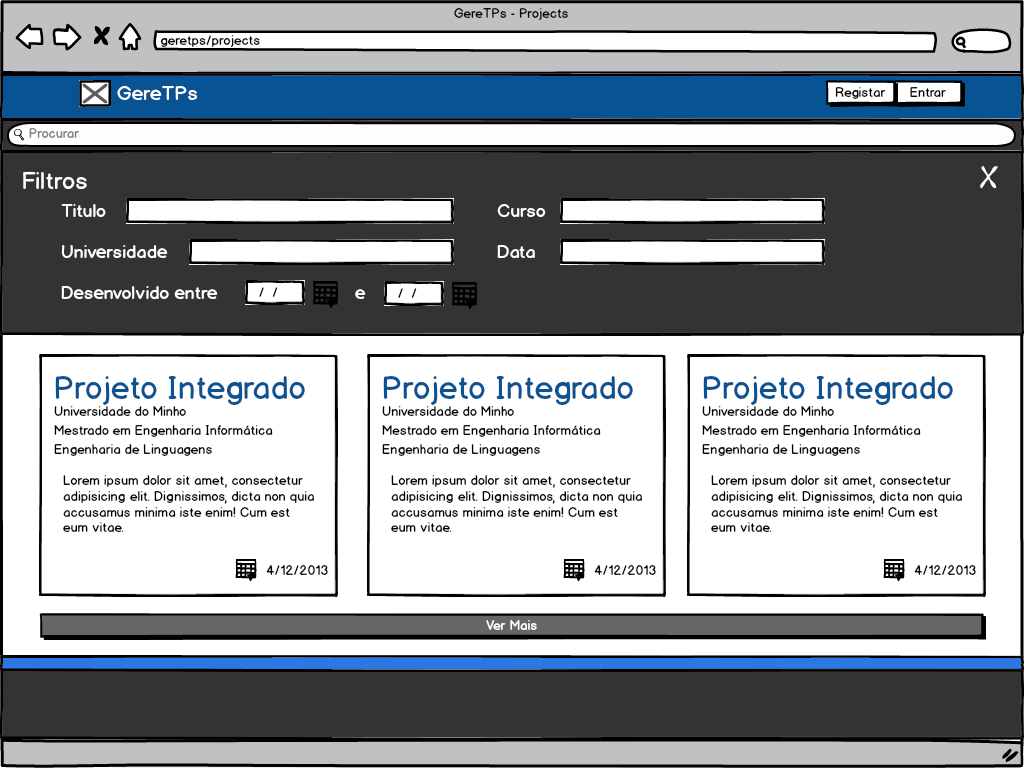
\includegraphics[width=1\textwidth]{images/prototipos/mockups/Projetos.png}
         \caption{Listagem dos projetos públicos}
         \label{fig: projetospublicos}
\end{figure}

Quando dentro do painel de um projeto, um docente pode:

\begin{itemize}
        \item Alterar informações do projeto
	\item Adicionar um enunciado, tal como outros ficheiros
	\item Gerir os grupos criados dentro do projeto
	\item Gerir as fases do projeto
	\item Consultar as submissões feitas até ao momento
        \item Adicionar/Remover testes
\end{itemize}
tal como se pode ver na Figura ~\ref{fig: painelprojetodocente}.\\

\begin{figure}[H]
        \centering
        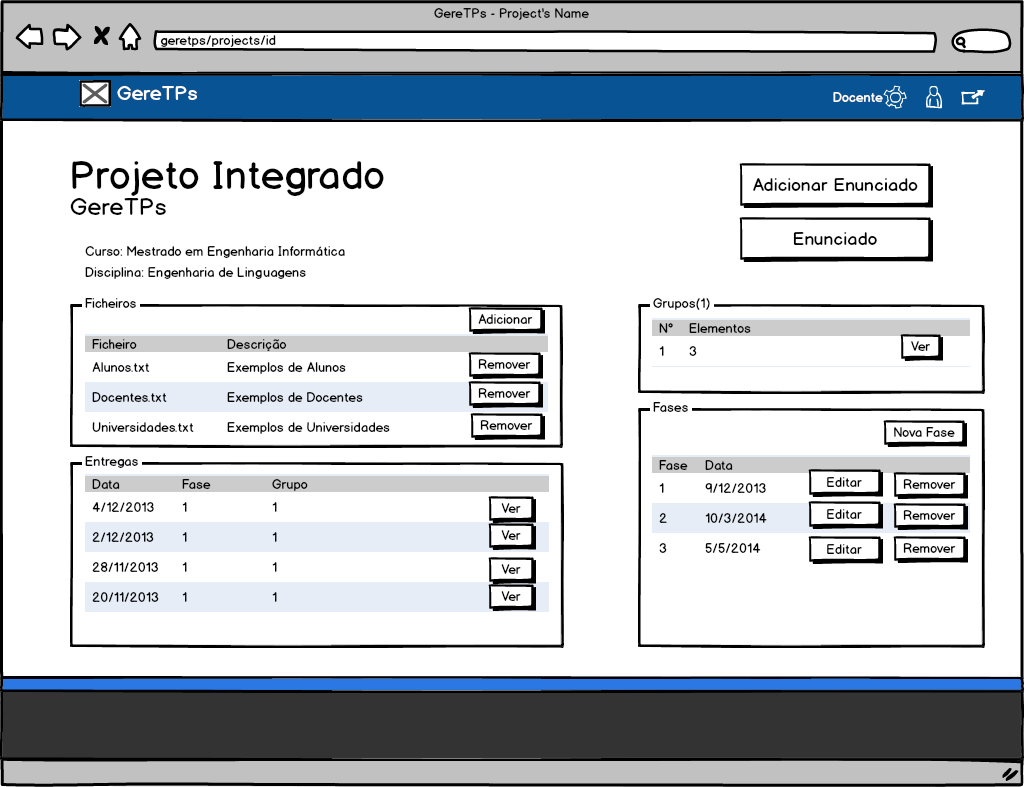
\includegraphics[width=1\textwidth]{images/prototipos/mockups/painelprojetodocente.png}
         \caption{Painel de projeto de um docente}
         \label{fig: painelprojetodocente}
\end{figure}

Um aluno pode consultar as informações dadas pelos os docente, consultar as entregas efetuadas pelo grupo, fazer a gestão do seu grupo e aceder a página de submissão de um projeto, como é possível ver na Figura ~\ref{fig: painelprojetoaluno}.\\

\begin{figure}[H]
        \centering
        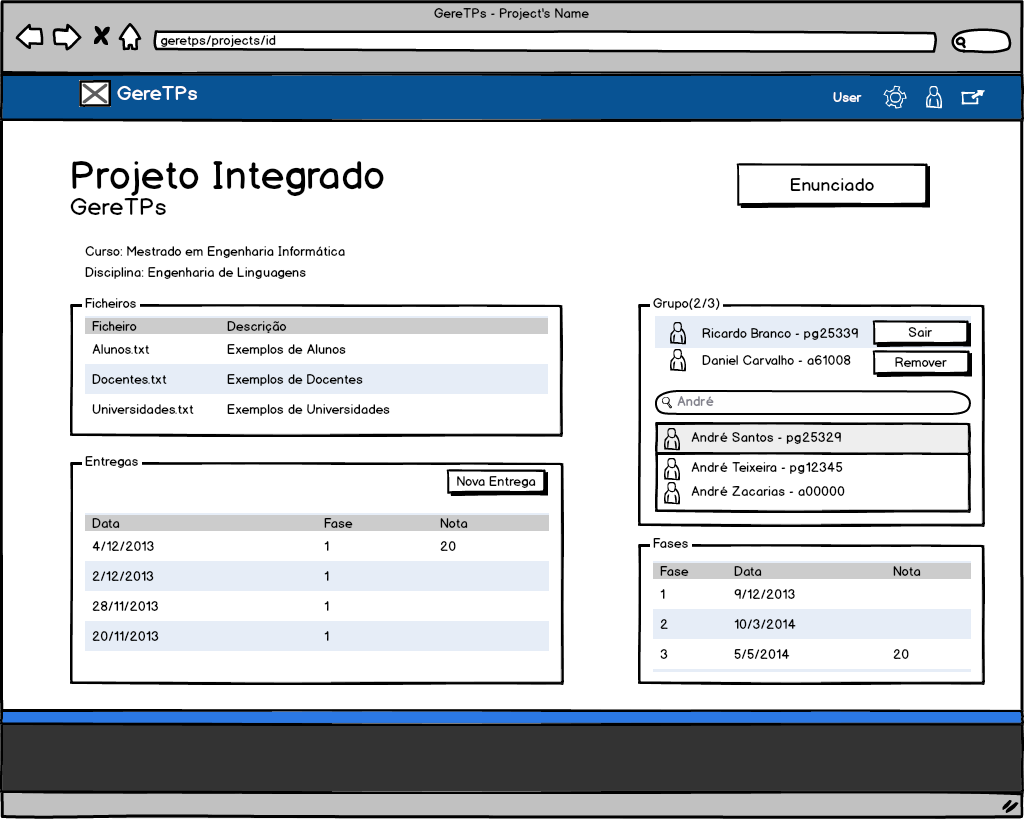
\includegraphics[width=1\textwidth]{images/prototipos/mockups/painelprojetoaluno.png}
         \caption{Painel de projeto de um aluno}
         \label{fig: painelprojetoaluno}
\end{figure}

Quando se visualiza um projeto, e de acordo com a Figura ~\ref{fig: projetoaluno}, pode-se aceder diretamente ao enunciado e relatório do projeto, ver e fazer \emph{Dowload} individual ou global(Ficheiro \emph{ZIP}) dos ficheiros submetidos, também é disponibilizado um resumo sob o trabalho feito, assim como a nota deste caso exista.Se for um docente responsável pela disciplina em que se enquadra o projeto a aceder à página, este pode fazer a avaliação do grupo, ou de cada membro individual e adicionar comentários sob a nota dada, tal como podemos ver na Figura ~\ref{fig: projetodocente}.\\

\begin{figure}[H]
        \centering
        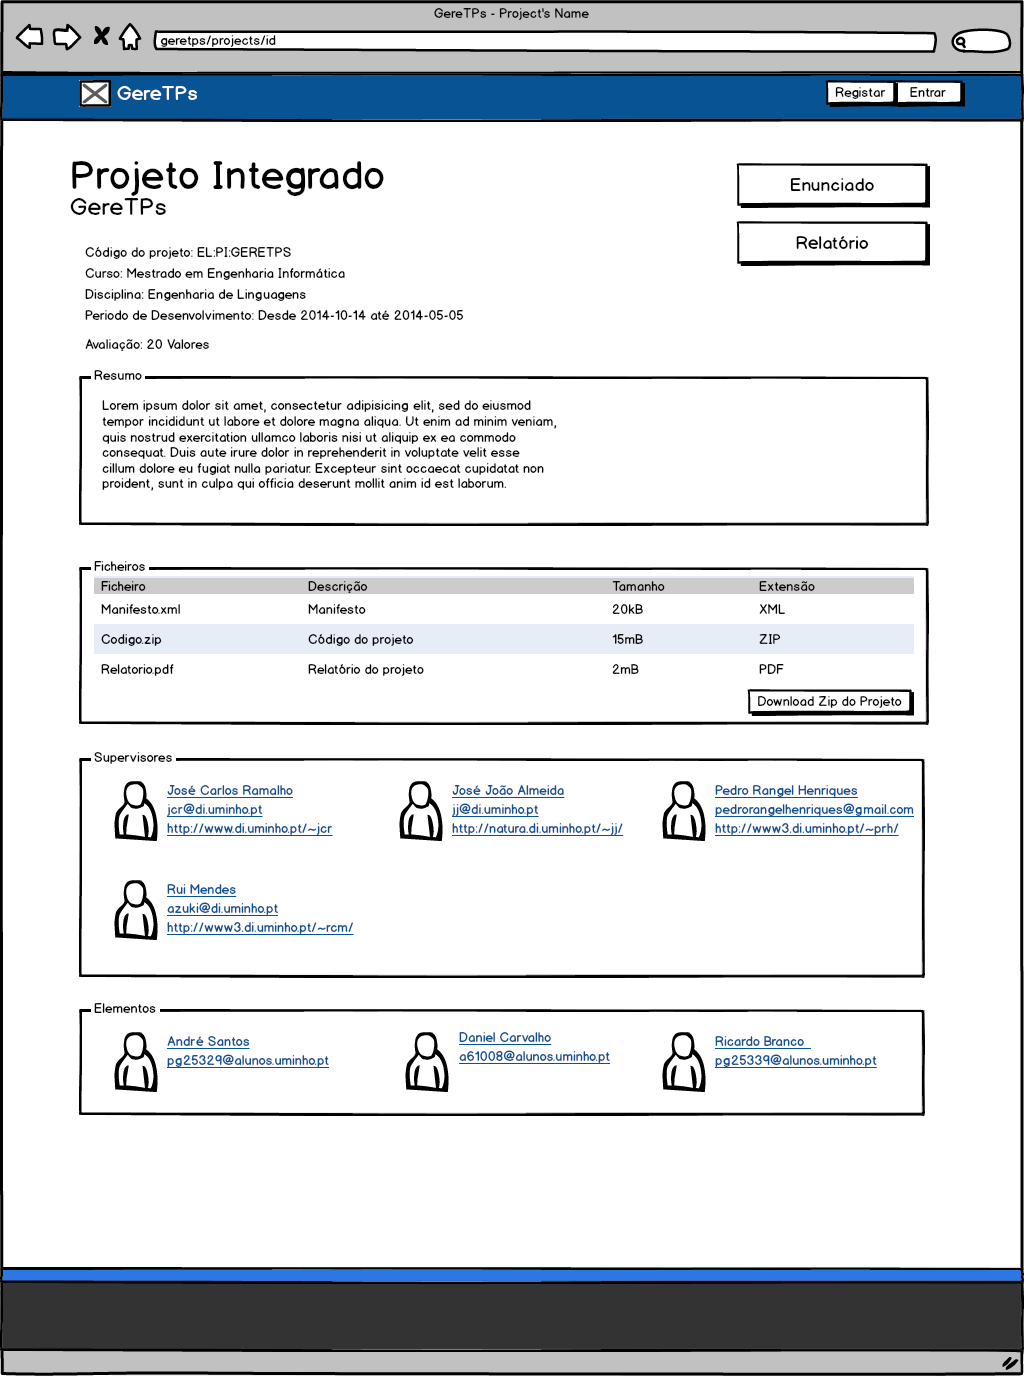
\includegraphics[width=1\textwidth]{images/prototipos/mockups/projetovisitante.png}
         \caption{Entrega vista por um visitante}
         \label{fig: projetoaluno}
\end{figure}

\begin{figure}[H]
        \centering
        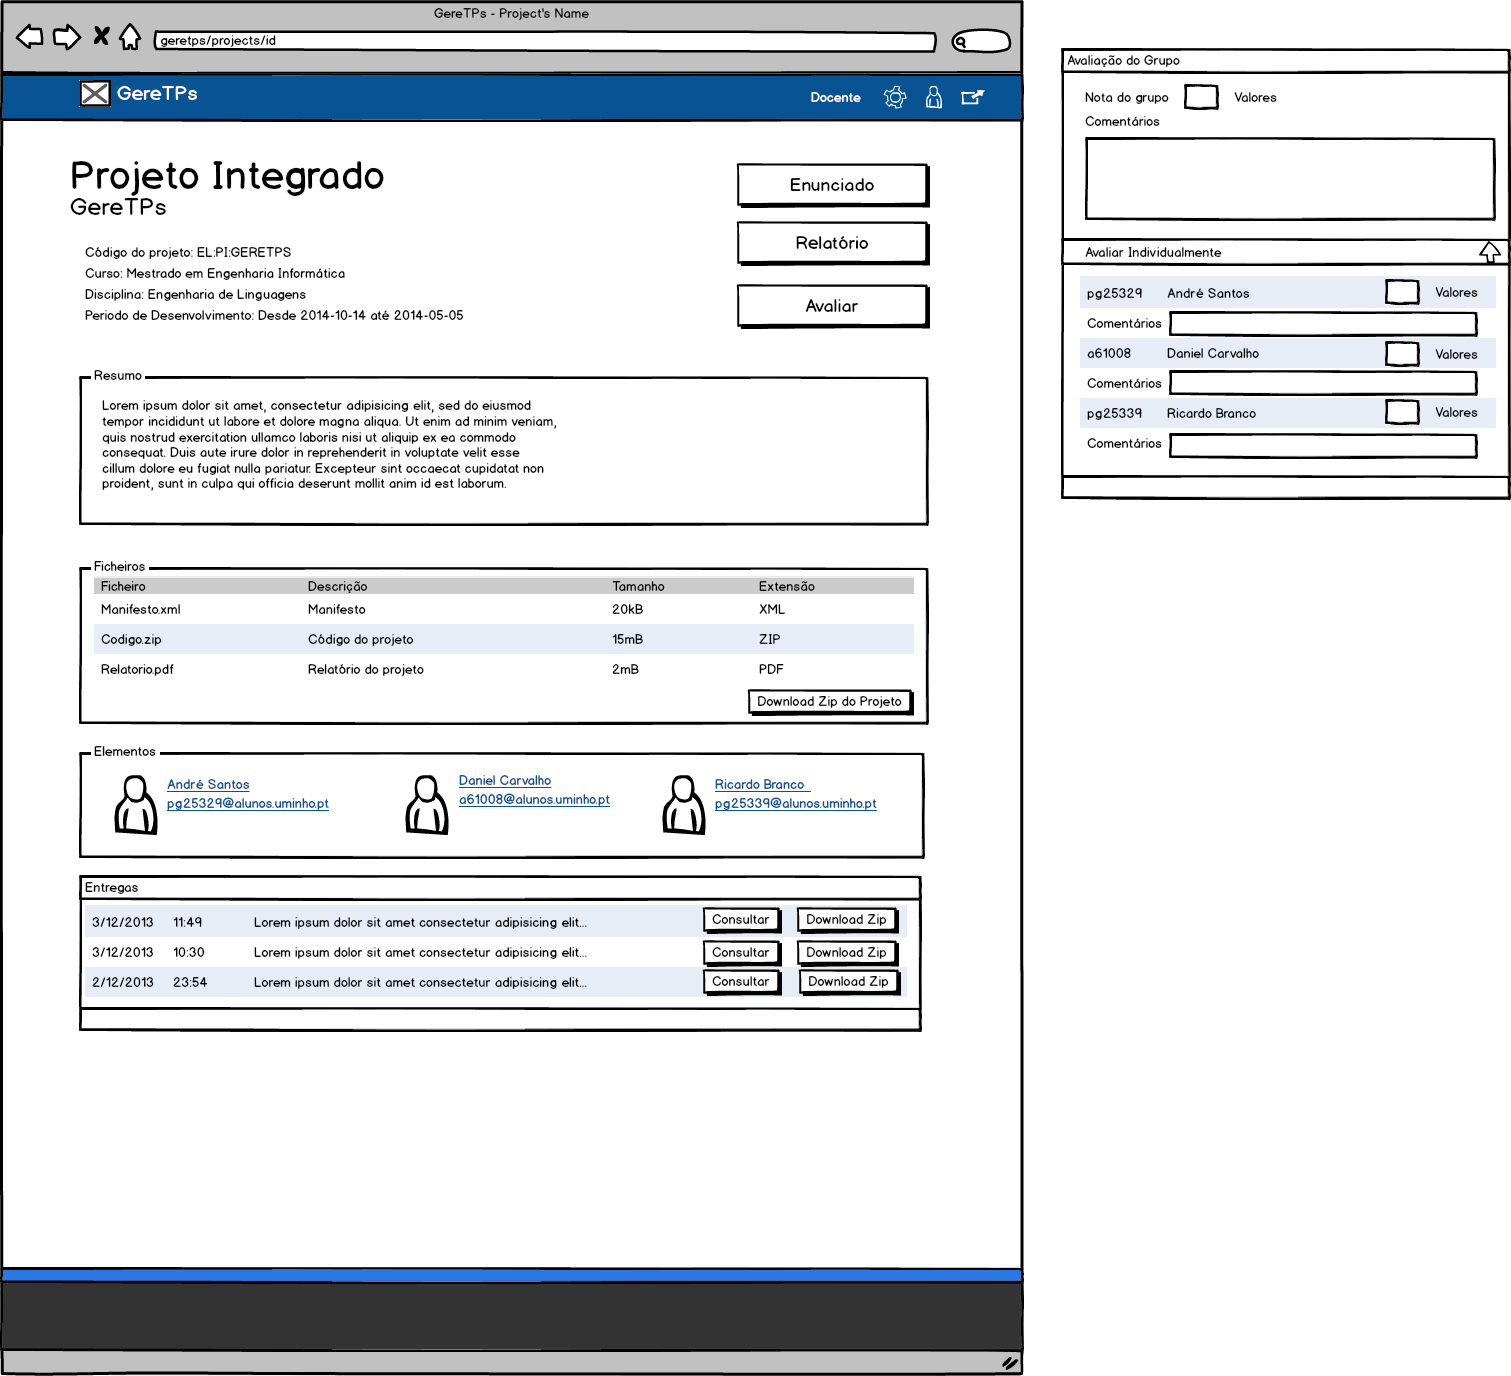
\includegraphics[width=1\textwidth]{images/prototipos/mockups/projetodocente.png}
         \caption{Entrega vista por um docente}
         \label{fig: projetodocente}
\end{figure}

\subsection{Protótipos fidedignos}
Para além dos primeiros protótipos, fizeram-se também protótipos fidedignos baseados nos anteriormente
citados de forma a aumentar o nível de detalhe, bem como aproximar a prototipagem o mais 
próximo possível do resultado final esperado. Assim sendo, segue-se na figura \ref{fig:prot_fid_home}
um exemplo da prototipagem fidedigna da página principal.
Com este tipo de protótipos espera-se aprimorar os detalhes, bem como os esquemas de cores,
arranjos gráficos, entre outros pormenores.
De notar que os protótipos fidedignos feitos neste projeto foram construídos diretamente a partir
da linguagem HTML.

\begin{figure}[H] 
  \centering
  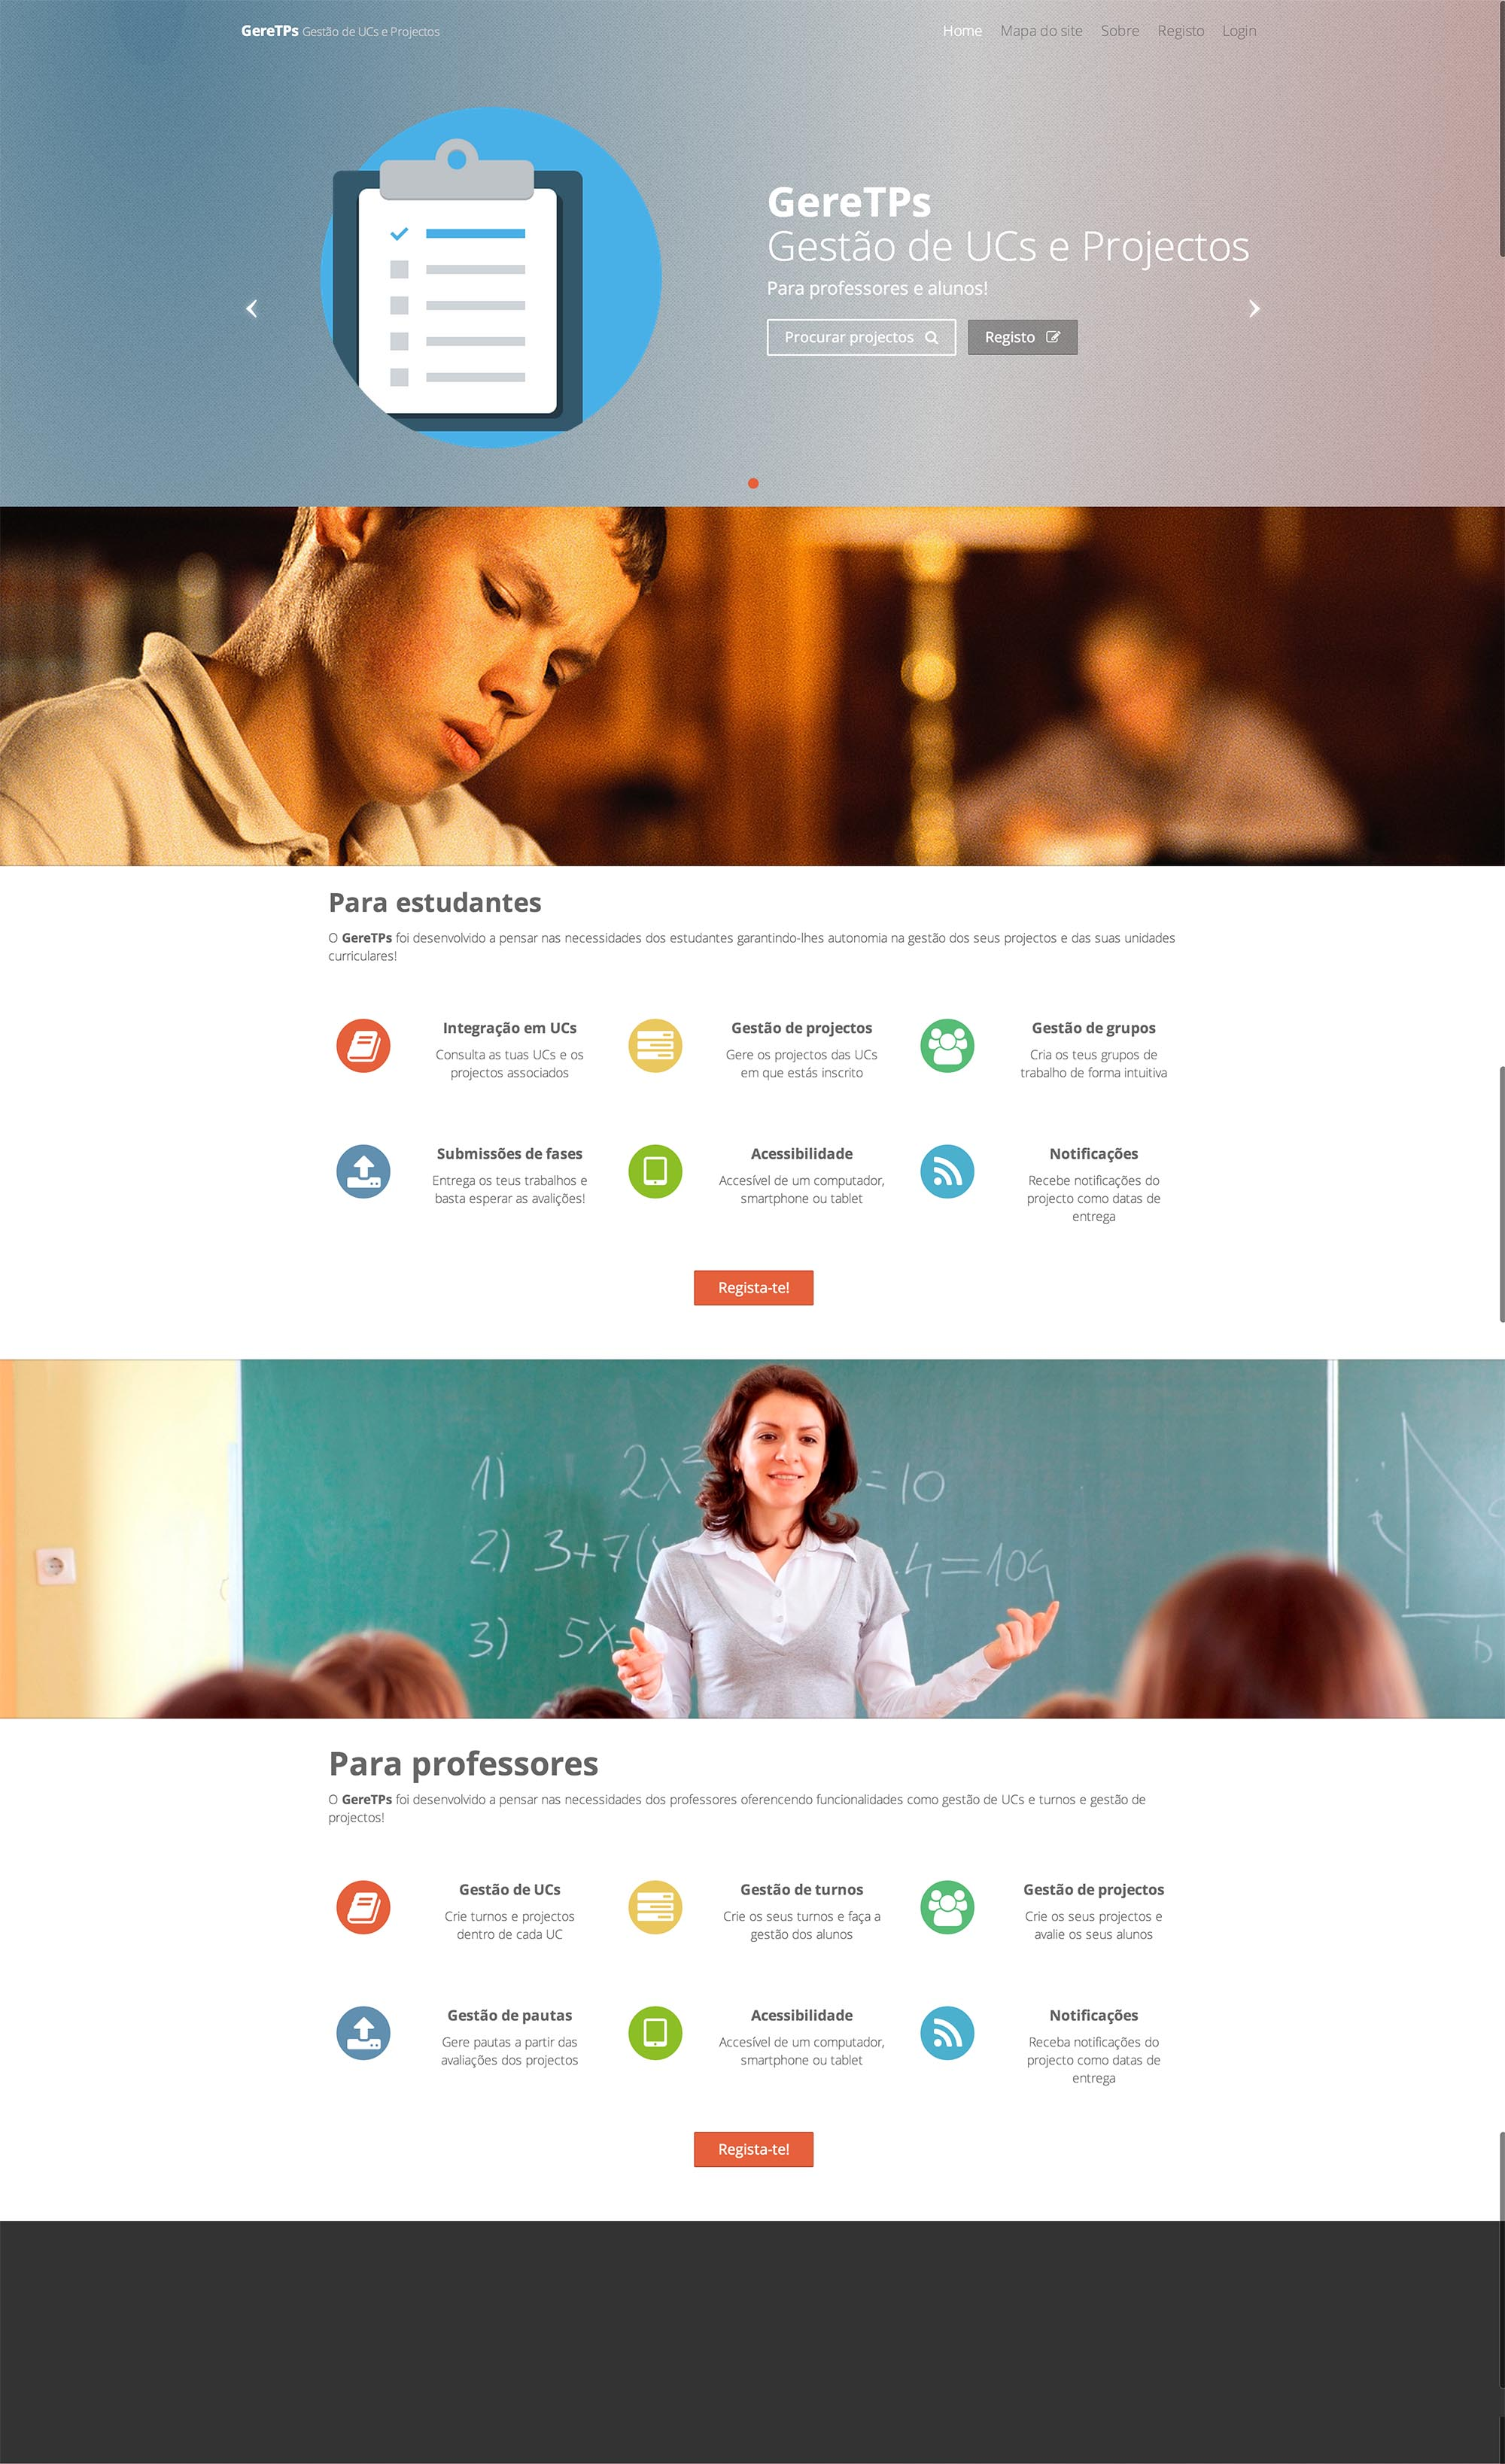
\includegraphics[width=0.8\textwidth,center]{images/prototipos/fidedigno_home.jpg}
  \caption{Protótipo fidedigno página inicial}
  \label{fig:prot_fid_home}
\end{figure}

\newpage


\section{Proposta tecnológica}

Para o desenvolvimento do nosso sistema, precisamos de combinar um vasto conjunto de tecnologias que permitam 
simplificar o desenvolvimento de todas as funcionalidades propostas.

De forma a organizar o fluxo de trabalho do grupo, utilizamos o \href{https://trello.com/}{\textbf{Trello}}, 
que é um sistema para gestão de tarefas que segue o método \textit{kanban}.
\begin{figure}[H] 
  \centering
  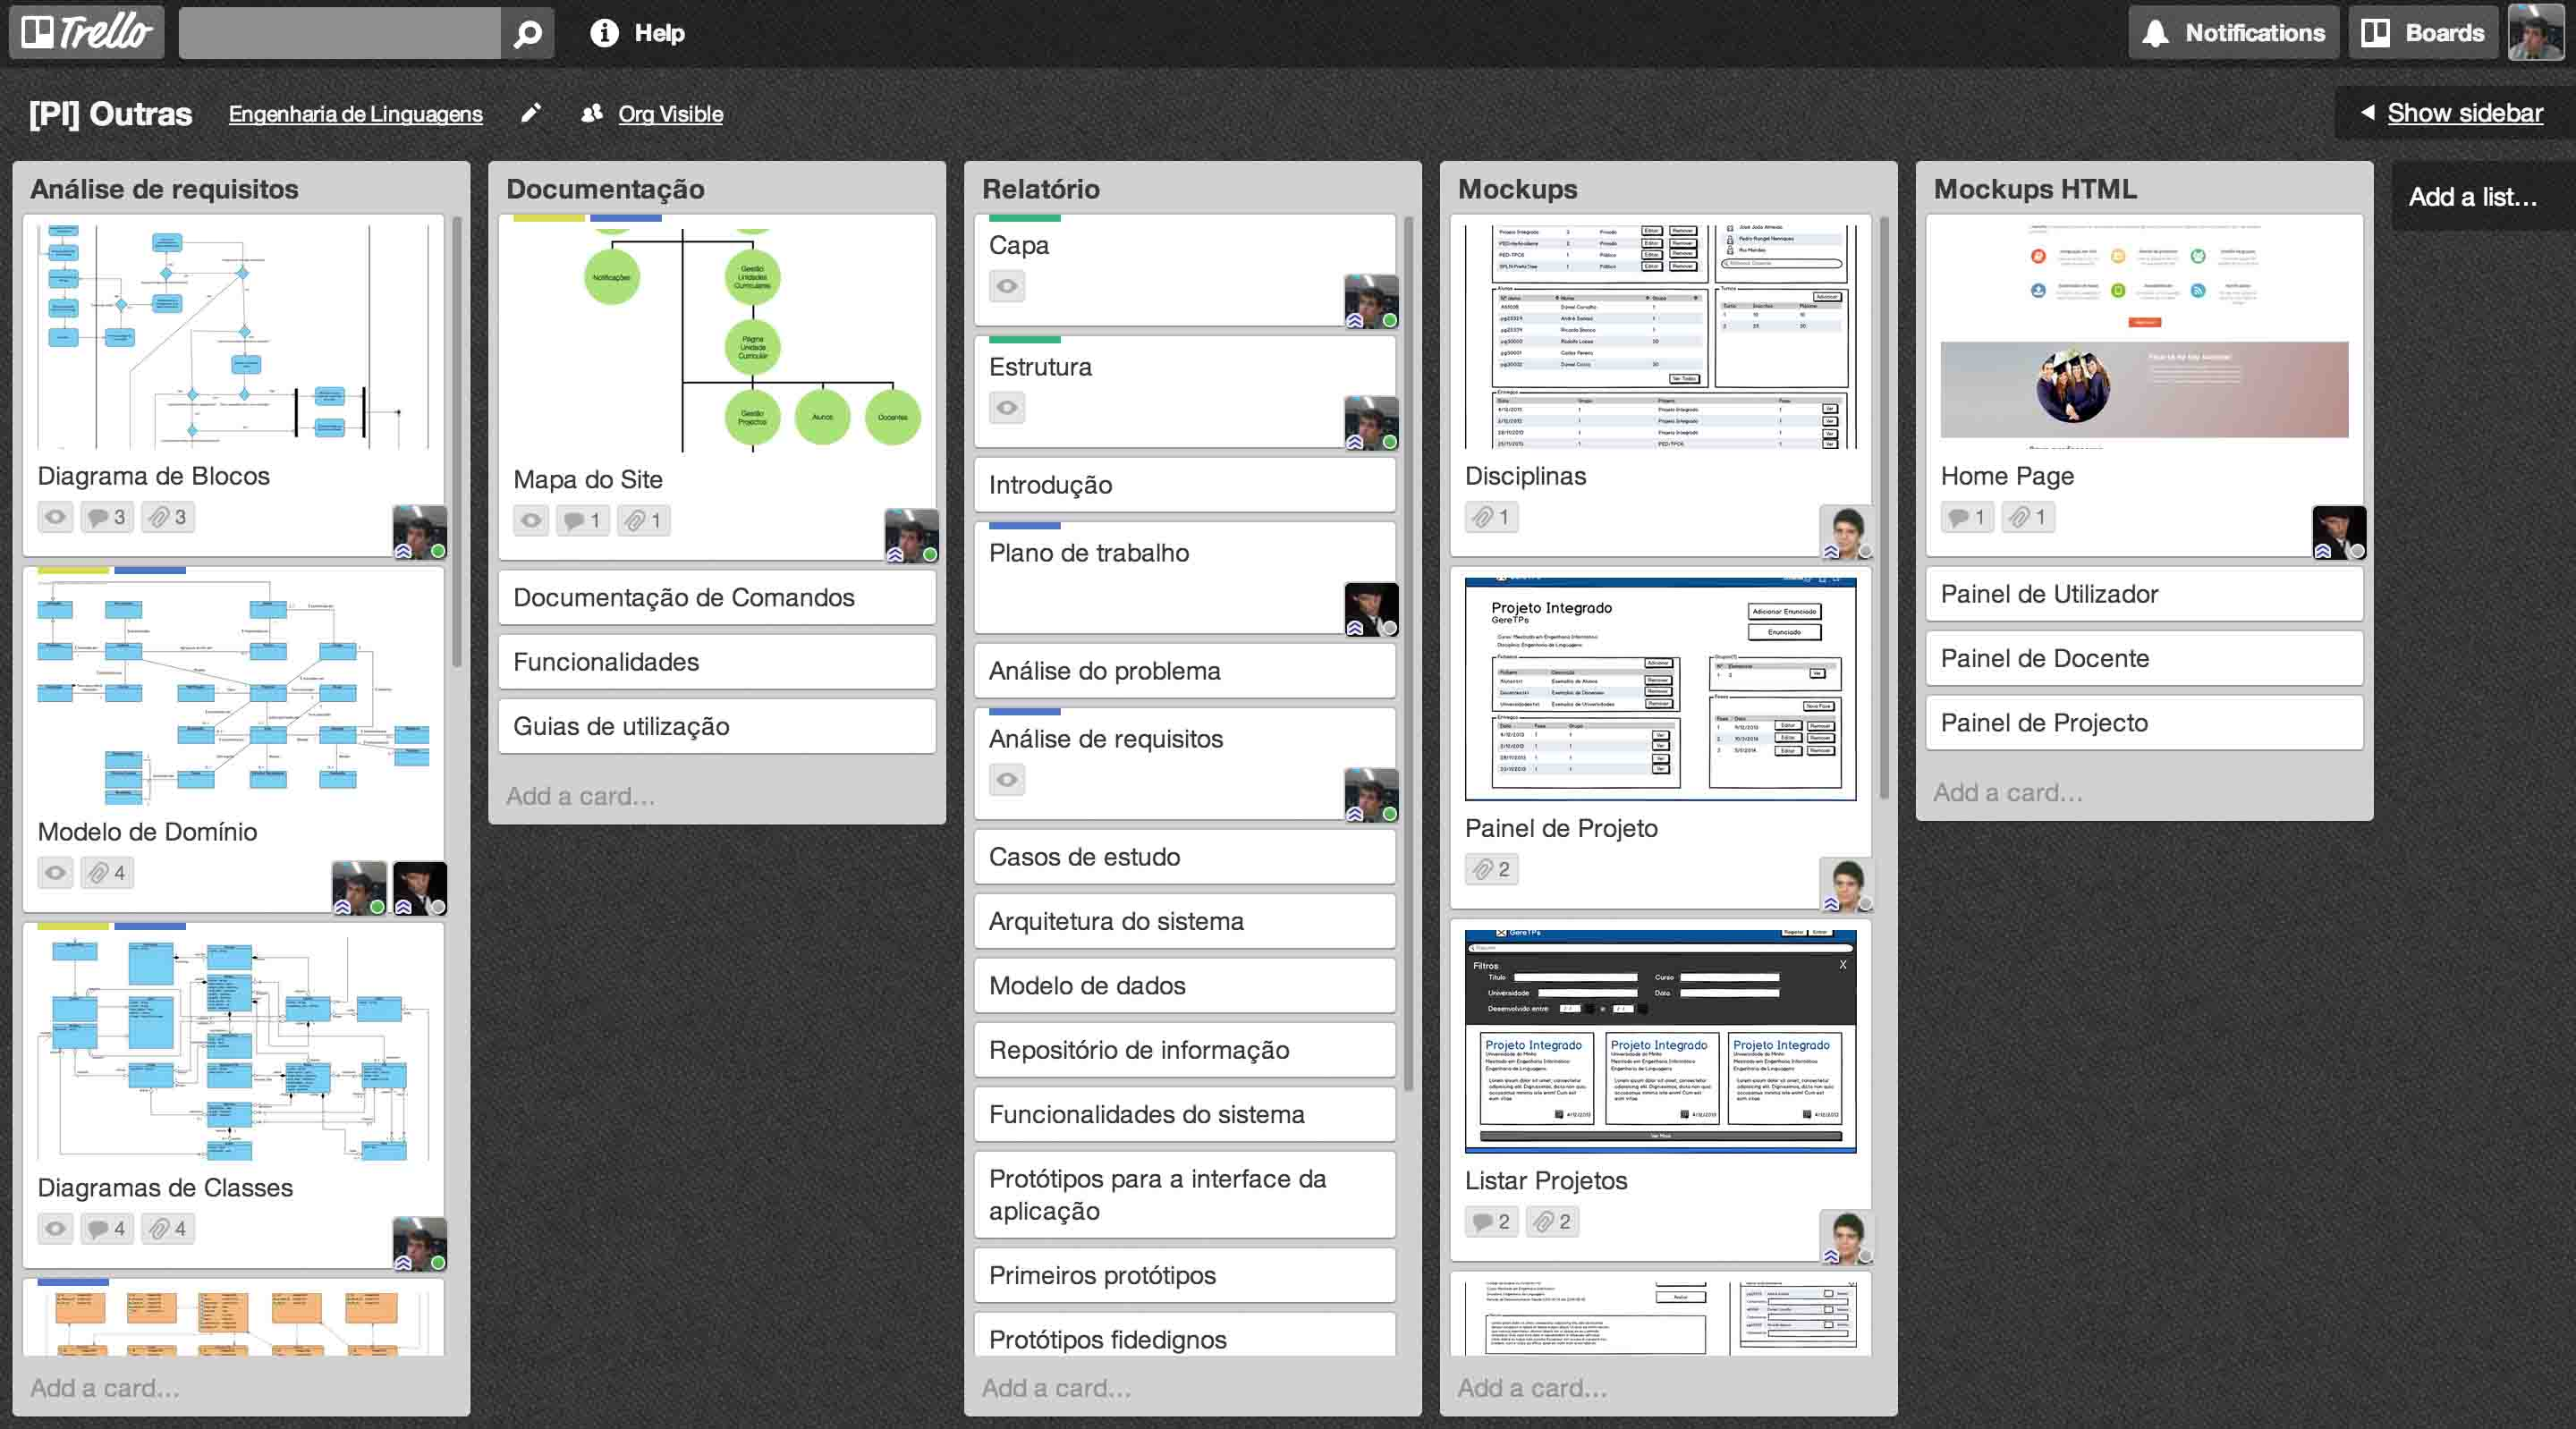
\includegraphics[width=1\textwidth]{images/tecnologias/trello}
  \caption{Trello}
  \label{fig:trello}
\end{figure}

Para o controlo de versões utilizaremos \textbf{Git}, que é um sistema de controlo de versões 
centralizado que apresenta as seguintes características:

\begin{itemize}
  \item Suporte consistente para desenvolvimentos não-lineares
  \item Desenvolvimento distribuído
  \item Compatibilidade com protocolos/sistemas existentes
  \item Manipulação eficiente de projetos extensos  
  \item Autenticação criptográfica do histórico 
  \item Modelo baseado em ferramentas 
  \item Estratégias de mescla (merge) conectáveis
  \item Empacotamento periódico explícito de objetos  
\end{itemize}

Para armazenar o código do nosso projeto vamos utilizar o \href{http://github.com}{\textbf{Github}}, 
que é um serviço de \textit{web hosting} o para projetos que usam o \textbf{Git} como sistema de controle de versões. 
Iremos utilizar um sistema de \textit{\textbf{Pull Requests}} e \textit{\textbf{Code Reviews}} 
para que assim todos os elementos possam ver e discutir o código produzido.

Procuraremos respeitar um dos fluxos de trabalho baseados em Git mais conhecidos, 
o \href{https://www.atlassian.com/git/workflows#!workflow-feature-branch}{\textbf{\textit{Feature Branch Workflow}}} 
que pode ser representado pela figura ~\ref{fig:git-workflow}.

\begin{figure}[H] 
  \centering
  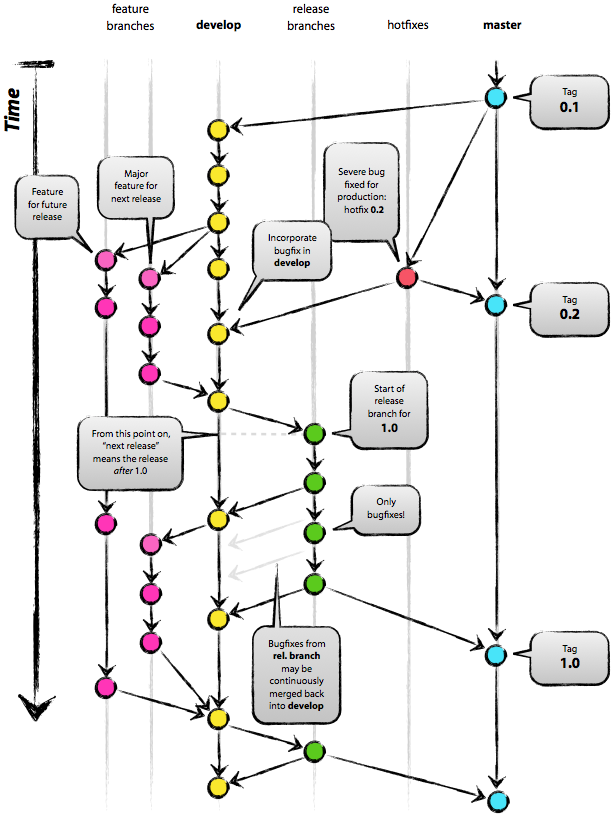
\includegraphics[width=0.5\textwidth]{images/tecnologias/git-workflow}
  \caption{Feature Branch Workflow}
  \label{fig:git-workflow}
\end{figure}

Relativamente ao desenvolvimento, utilizaremos \href{http://rubyonrails.org/}{\textbf{Ruby on Rails}}, 
que é uma \textit{framework open-source} escrita em \textbf{Ruby}, otimizada para a produtividade sustentável. 
A \textit{framework} tem uma forte comunidade que defende conceitos como \textbf{DRY} \textit{(Don't Repeat Yourself)} 
e \textbf{\textit{Convention over configuration}}.

\textbf{Ruby on Rails} é uma \textit{meta-framework}, composta pelos seguintes \textbf{frameworks}:

\begin{description}[labelindent=1cm]
  \item[Active Record] Responsável pela interoperabilidade entre a aplicação e a base de dados, e pela abstração dos dados.
  \item[Action Pack] Compreende o \textbf{Action View} (gera o que o utilizador vê, como HTML, XML e JavaScript) 
  e o \textbf{Action Controller} (controle do fluxo de negócio).
  \item[Action Mailer] Responsável pelo serviço de entrega e receção de e-mails.
  \item[Active Support] Coleção de várias classes e bibliotecas, que foram considerados úteis para aplicações em Ruby on Rails.
\end{description}

Para além das \textit{frameworks} indicadas iremos recorrer a \textbf{Gems} para simplificar alguns processos, tais como:

\begin{description}[labelindent=1cm]
  \item[Devise] Autenticação de utilizadores.
  \item[Paperclip] Upload e validação de imagens e arquivos.
  \item[Capistrano] Automatização de processos de implantação \textit{(deployment)}.
  \item[Nokogiri] Parser de HTML e XML com XPath e seletores CSS.
  \item[XML-Simple] API simples para trabalhar com documentos XML.
\end{description} 

Pretendemos melhorar a nossa produtividade, e melhorar a legibilidade do código produzido utilizando os seguintes pré-processadores:

\begin{description}[labelindent=1cm]
  \item[\href{http://slim-lang.com/}{Slim}] para HTML.
  \item[\href{http://sass-lang.com/}{SASS}] para CSS.
  \item[\href{http://coffeescript.org/}{CoffeeScript}] para JavaScript.
\end{description} 

Utilizaremos a \textit{framework} de \textit{front-end} \href{http://getbootstrap.com/}{\textbf{Twitter Bootstrap}} 
para ajudar a construirmos um serviço multi-plataforma e para reutilizarmos alguns componentes.
Para além disso também utilizaremos a biblioteca de Javascript \href{http://jquery.com/}{\textbf{JQuery}} para simplificar os \textit{scripts client side} que interagem com o HTML.\\

Para manipulação de documentos \textbf{XML}, utilizaremos as tecnologias lecionadas, tais como: \textbf{DTD}, \textbf{XSLT} e \textbf{XSD}.\\

Relativamente a tecnologias de Base de Dados, utilizaremos bases de dados SQL, mais especificamente \href{http://www.sqlite.org/}{\textbf{SQLite}} 
para ambientes de teste e desenvolvimento, e \href{http://www.postgresql.org/}{\textbf{PostgreSQL}} para ambientes de produção.

\newpage

\section{Soluções implementadas}

Nesta secção serão referidas todas as soluções já implementadas para o problema descrito.

Serão demonstradas todas as páginas e funcionalidades já implementadas, com justificações para as decisões tomadas.

\subsection{Página inicial}

Esta página é dirigida a todos os utilizadores e visitantes do sistema, é a primeira página e não é necessário ter um registo no sistema para a consultar.

Nesta página pretende-se demonstrar todas as funcionalidades do sistema, cativar novos utilizadores e promover a aplicação.\\

No inicio da página optou-se por colocar um \textit{slider} que de uma forma simples e sucinta explicita as principais vantagens do sistema como ser acessível em qualquer dispositivo e principais vantagens para os alunos e para os docentes.

De seguida são listados os diferentes tipos de utilizadores para os quais o sistema oferece vantagens, e uma frase que pretende cativar esse grupo de utilizadores a utilizar o sistema.

Como os estudantes constituem a maior parte dos potenciais utilizadores do sistema, decidiu-se listar as principais categorias onde estes utilizadores vão obter mais vantagens ao utilizar a aplicação.

Depois de frases de incentivo ao registo e imagens demonstrativas, são listadas as categorias onde os docentes vão obter mais vantagens ao utilizar a aplicação.\\

Nesta página os utilizadores não registados, para além de consultar as funcionalidades do sistema, podem aceder ao mapa do site, sobre nós, pesquisar por projetos públicos e entrar ou registar no sistema.
Os utilizadores registados para além das possibilidades referidas, podem aceder a um painel de gestão de projetos e unidades curriculares.\\ 

Na Figura~\ref{fig:home_page} pode ser consultada uma imagem demonstrativa da página desenvolvida.\\

\begin{figure}[H]
  \centering
  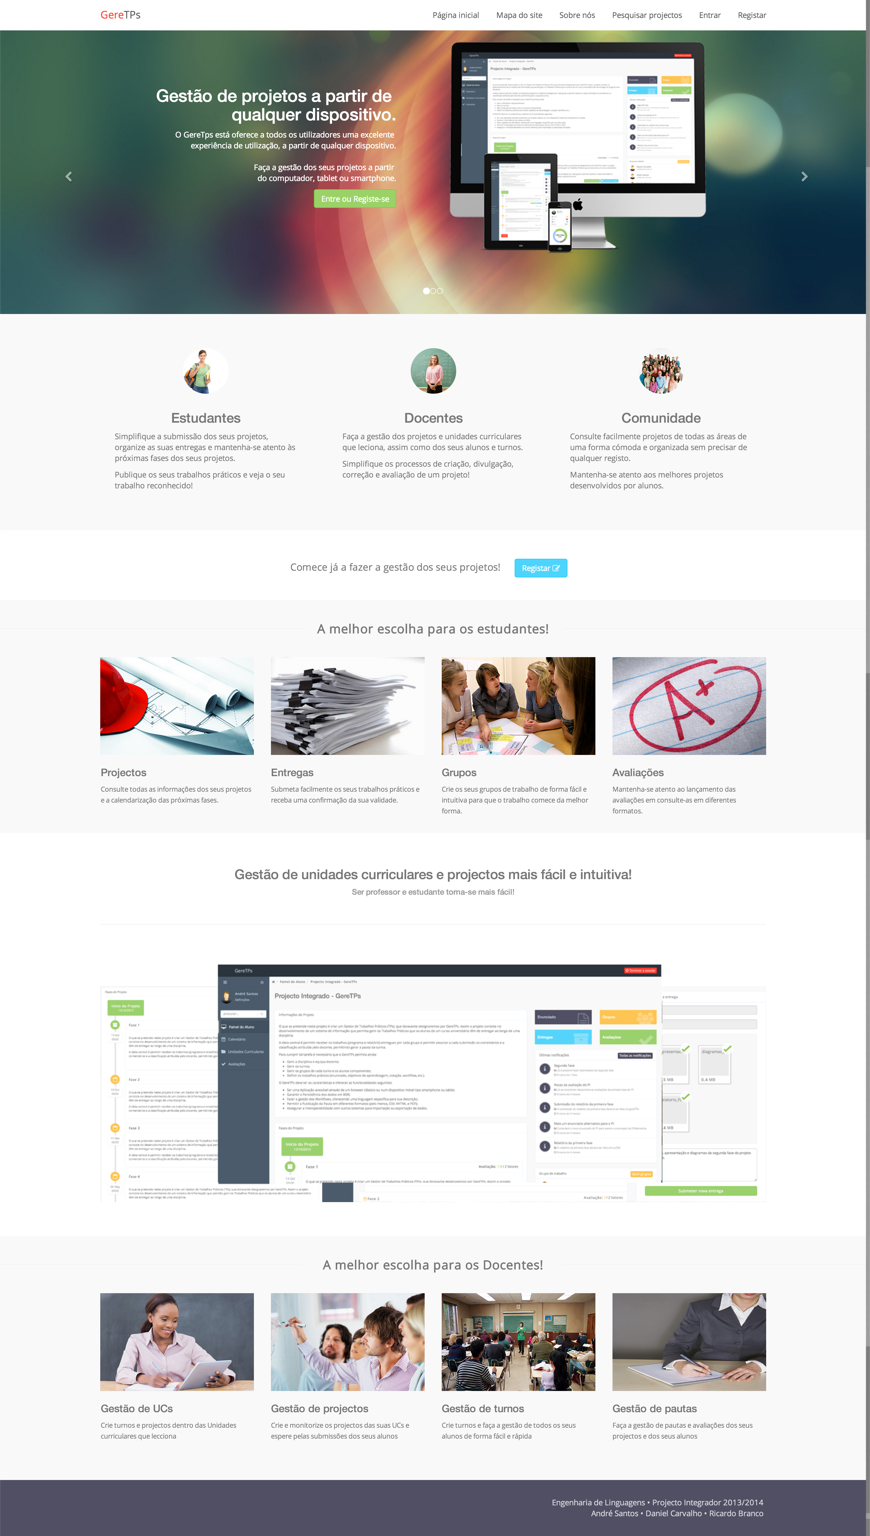
\includegraphics[width=.7\textwidth,center]{images/implementacao/home_page}
  \caption{Página inicial}
  \label{fig:home_page}
\end{figure}

\subsection{Página de login}

\subsection{Pagina de registo}

Esta página permite que os utilizadores não registados, efetuem o registo no sistema para poderem aceder a todas as funcionalidades.\\

Para efetuar o registo, um utilizador apenas precisa de indicar os campos essenciais para utilizar o sistema, nome, email, número de aluno (se indicar que é estudante), telemóvel e \textit{password}.
Os restantes campos que compõem a informação do utilizador, como descrição e fotografia, podem ser preenchidos posteriormente, na edição do perfil.\\

Depois do registo, os utilizadores serão direcionados para o painel do aluno ou docente, dependendo do tipo de utilizador que indicou.

Nesta página os utilizadores não autenticados podem regressar à página inicial, ao carregar no logótipo do sistema, ou aceder à página de autenticação.

O utilizador é notificado com mensagens de erro explicitas quando falhar o registo, indicando em que campo(s) ocorreram erros. 

Para esta página procurou-se um \textit{design} simples, onde o utilizador pode concentrar-se exclusivamente na funcionalidade pretendida, o registo.\\

Na Figura~\ref{fig:sign_up} pode ser consultada uma imagem demonstrativa da página desenvolvida.\\

\begin{figure}[H]
  \centering
  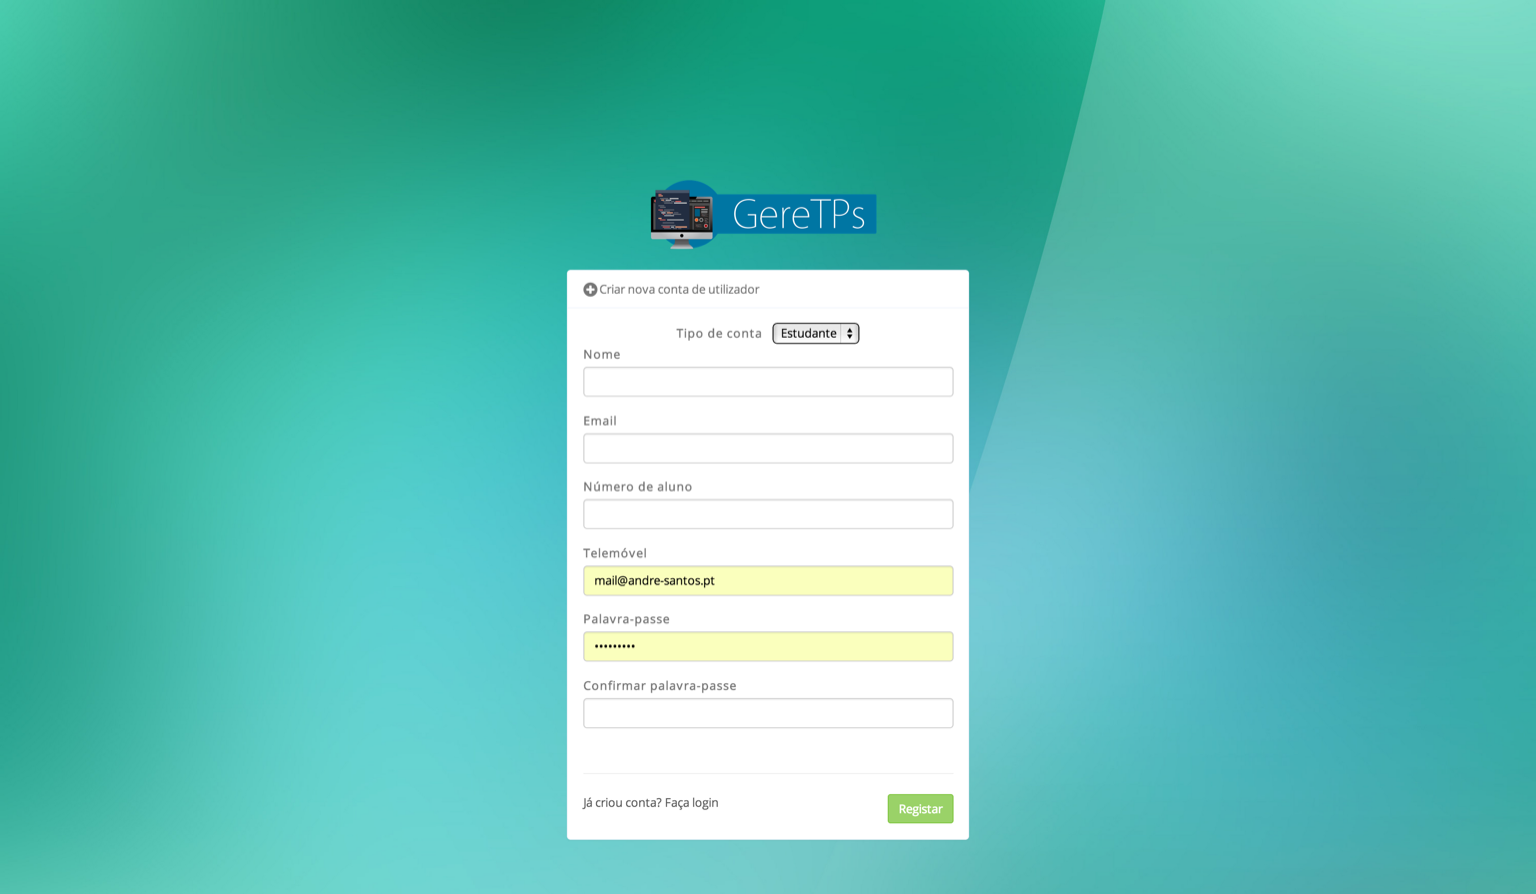
\includegraphics[width=1\textwidth,center]{images/implementacao/sign_up}
  \caption{Página de registo}
  \label{fig:sign_up}
\end{figure}

\subsection{Painel do aluno}

Nesta secção serão referidas todas as soluções já implementadas para o painel do aluno.

Serão demonstradas todas as páginas e funcionalidades já implementadas para este tipo de utilizadores, com justificações para as decisões tomadas.\\

Em todas as páginas, o aluno terá acesso a um cabeçalho onde poderá voltar à página inicial, ao carregar no logótipo, ou terminar a sua sessão no botão mais à direita.

Para além do referido cabeçalho o aluno terá acesso a uma barra lateral, onde poderá aceder às páginas de edição do perfil, página inicial do painel do aluno, calendário, gestão projetos, gestão de unidades curriculares e gestão de avaliações.

O aluno terá ainda acesso a uma barra de navegação que lhe permitirá saber sempre em que página do sistema se encontra, e voltar para páginas anteriores.

\subsubsection{Página inicial}

\subsubsection{Página de projeto}

\begin{figure}[H]
  \centering
  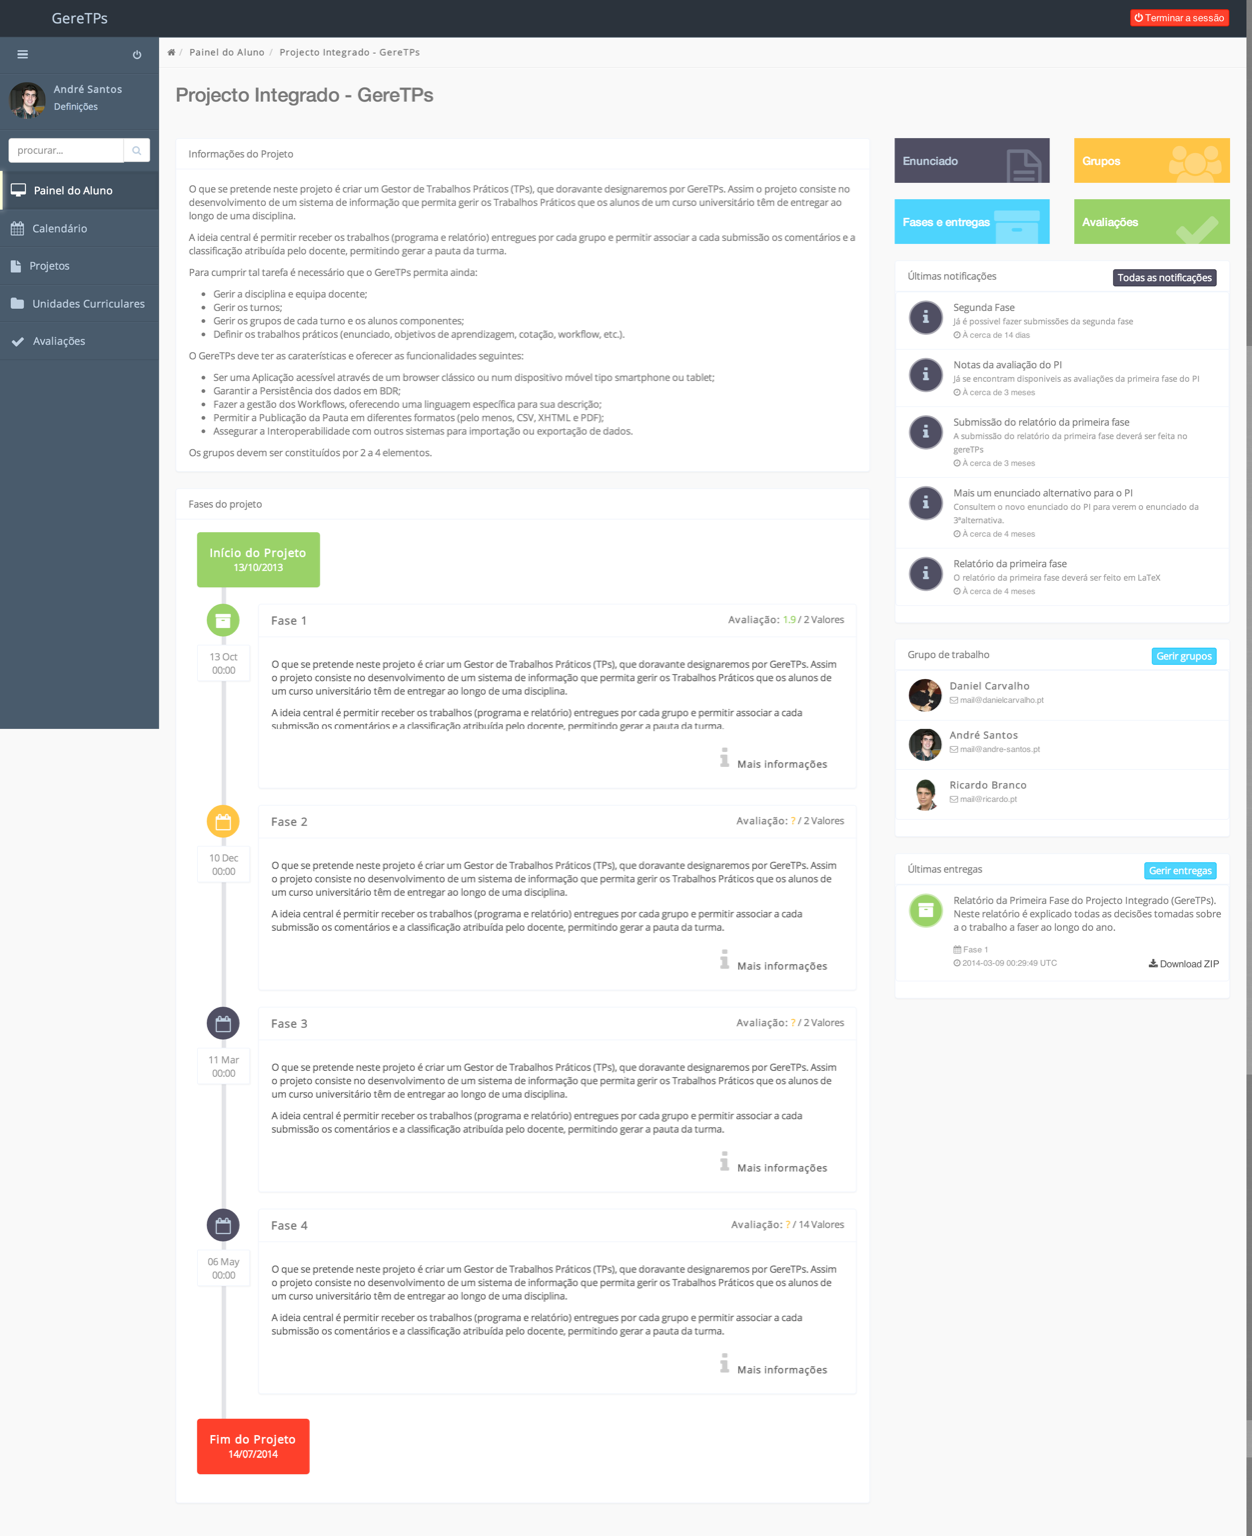
\includegraphics[width=1\textwidth,center]{images/implementacao/alunos/project}
  \caption{Página de projeto}
  \label{fig:student_project}
\end{figure}

\subsubsection{Gestão de grupos de trabalho}

\subsubsection{Gestão de fases e entregas}
\label{ssub:gestao_fases}

Na página dedicada à gestão de fases e entregas, um aluno pode consultar todas as informações das fases de um projeto, todas as entregas relativas às referidas fases e pode submeter novas entregas para a fase atual.

Sendo a submissão de entregas um dos processos mais críticos do sistema, pretende garantir-se a partir desta página mais flexibilidade e segurança para aluno ao longo deste processo.\\

Relativamente às fases, num plano principal, são apresentadas informações relativas às datas de inicio e de fim da fase, descrição, ficheiros de entrega obrigatória, ficheiros auxiliares, e atalhos para a pauta e para o enunciado da fase.

São ainda listadas todas as entregas para a referida fase.

Para cada entrega, o utilizador pode fazer \textit{download} de todos os ficheiros entregues como um ficheiro \textit{ZIP}.\\

Num painel mais à direita pode encontrar-se o formulário de submissão de nova entrega.

Esse formulário apenas será mostrado ao utilizador se forem verificadas duas restrições, pertencer a um grupo válido, e existir no momento uma fase ativa.

É importante referir que para uma submissão mais cómoda de ficheiros grandes, o utilizador pode carregar os ficheiros antes de proceder à submissão da entrega.

Optou-se por simplificar ao máximo o formulário de submissão de nova entrega, assim sendo, o utilizador apenas necessita de colocar os ficheiros e uma descrição da entrega.\\

Na Figura~\ref{fig:student_deliveries} pode ser consultada uma imagem demonstrativa da página desenvolvida.

\begin{figure}[H]
  \centering
  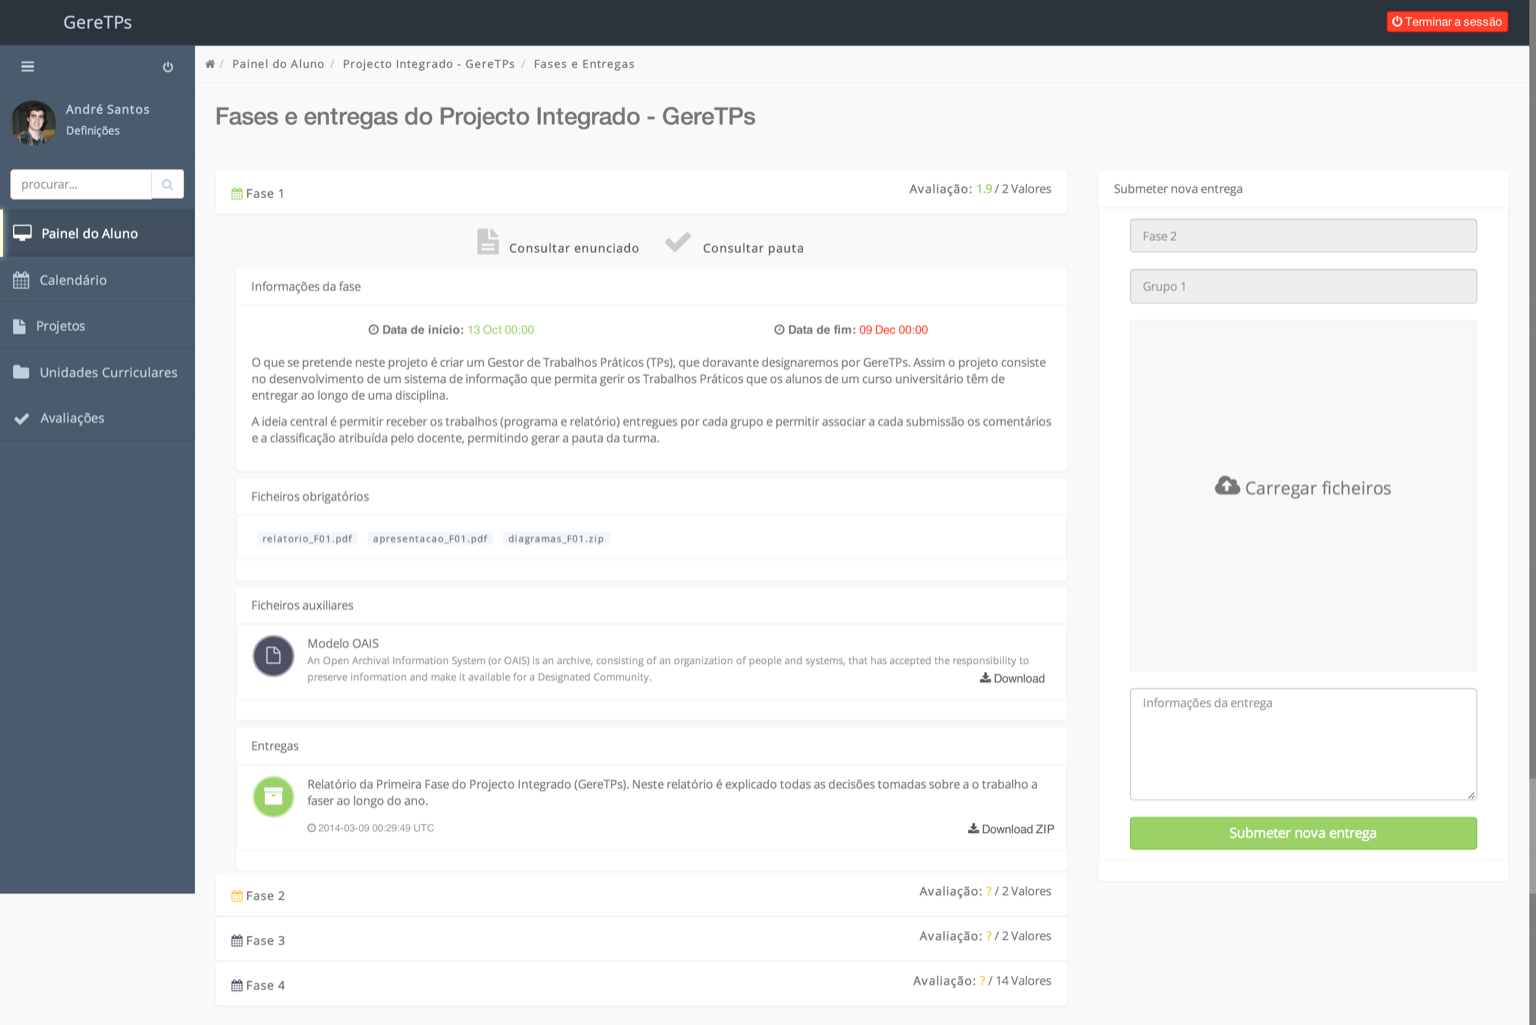
\includegraphics[width=1\textwidth,center]{images/implementacao/alunos/deliveries}
  \caption{Página de gestão de fases entregas}
  \label{fig:student_deliveries}
\end{figure}

\subsubsection{Pautas de fase e projeto}

No página de gestão de um projeto, um aluno pode consultar uma pauta detalhada. Esta pauta lista todos os alunos inscritos na unidade curricular associada ao projeto e respetiva nota.

Além da nota final do projeto, também é possível ver a nota de cada fase.

Na Figura~\ref{fig:student_grades_project} pode ser consultada uma imagem demonstrativa da página desenvolvida.

\begin{figure}[H]
	\centering
	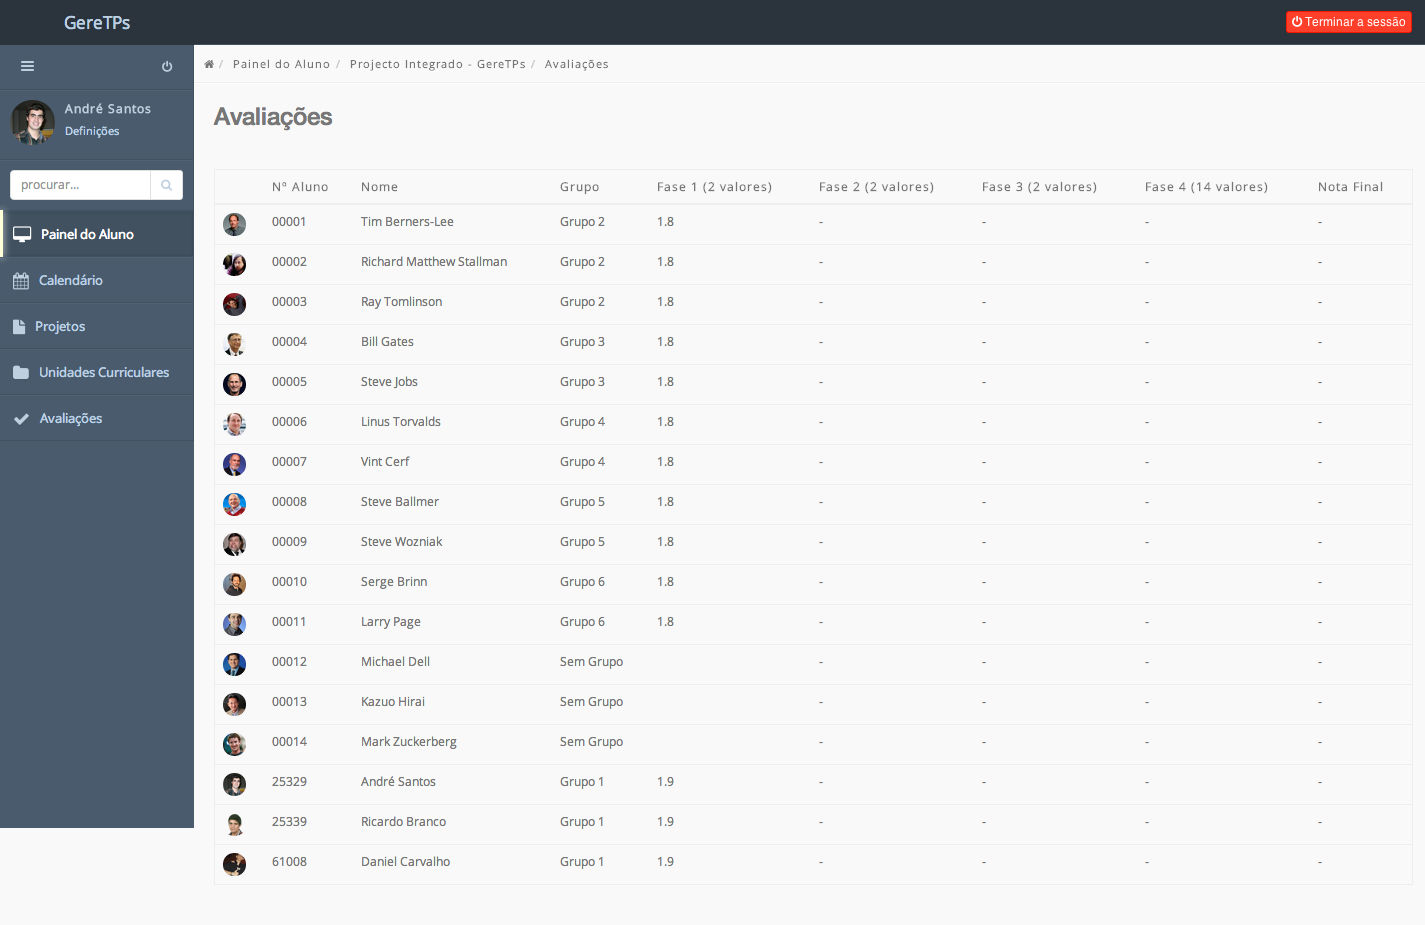
\includegraphics[width=1\textwidth,center]{images/implementacao/alunos/grades_project}
	\caption{Pauta de um projeto}
	\label{fig:student_grades_project}
\end{figure}

Ainda na página de gestão de um projeto, é possível aceder à página de \hyperref[ssub:gestao_fases]{Gestão de fases e entregas}. A partir desta página é possível um aluno consultar a pauta de uma fase de um projeto, caso esta já tenha sido lançada por um dos docentes da unidade curricular associada ao projeto.

A pauta de uma fase é bastante semelhante à pauta de um projeto, com a particularidade de esta apresentar a nota da fase entre zero e vinte valores e a nota correspondente no final do projeto.

Na Figura~\ref{fig:student_grades_phase} pode ser consultada uma imagem demonstrativa da página desenvolvida.

\begin{figure}[H]
	\centering
	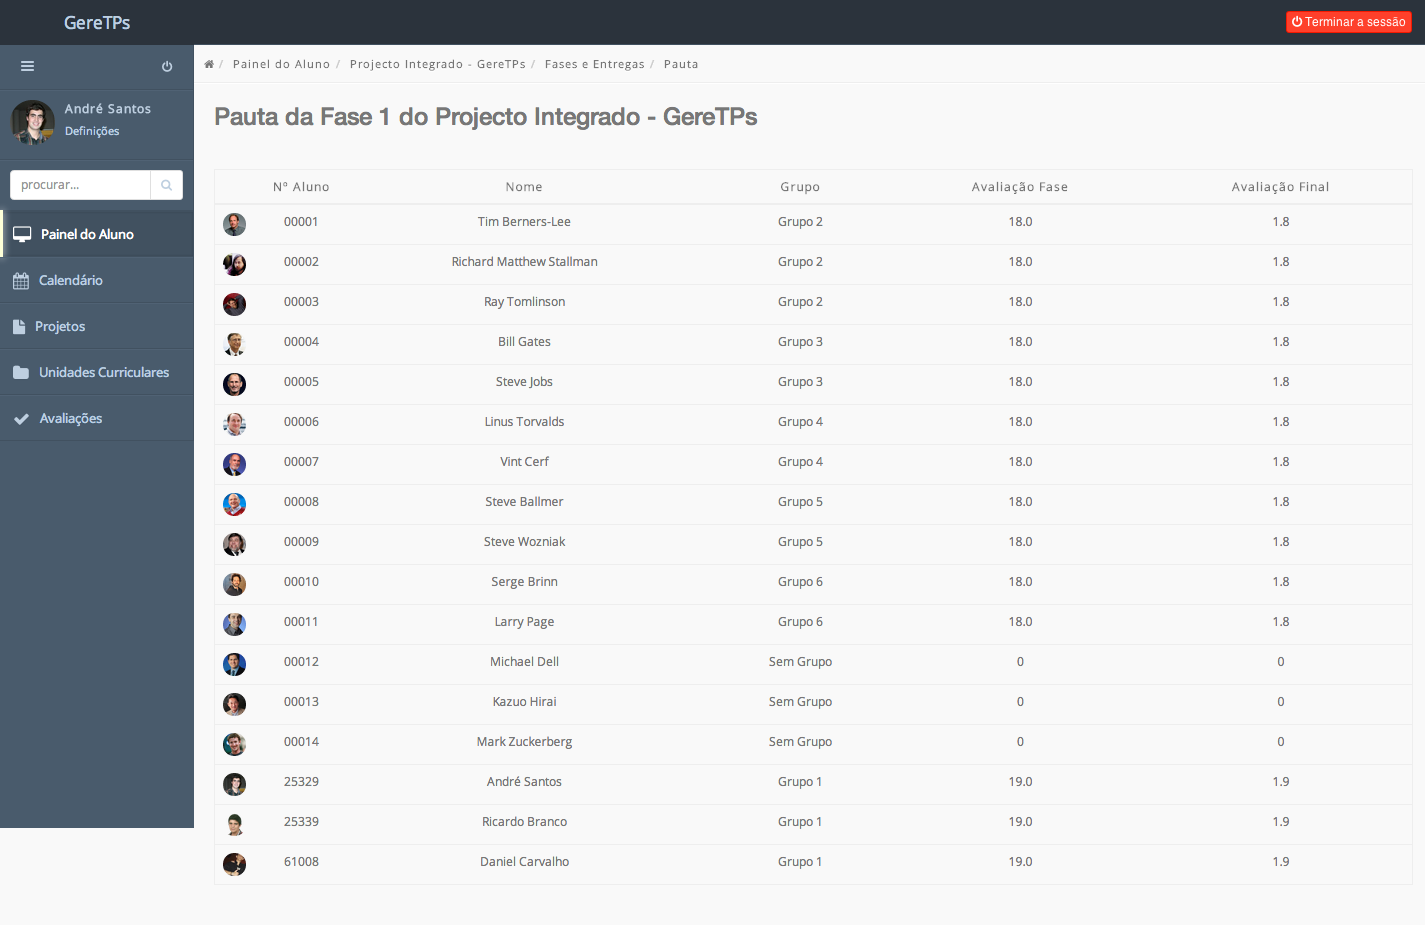
\includegraphics[width=1\textwidth,center]{images/implementacao/alunos/grades_phase}
	\caption{Pauta da uma fase}
	\label{fig:student_grades_phase}
\end{figure}

\subsubsection{Gestão de unidades curriculares}

\begin{figure}[H]
  \centering
  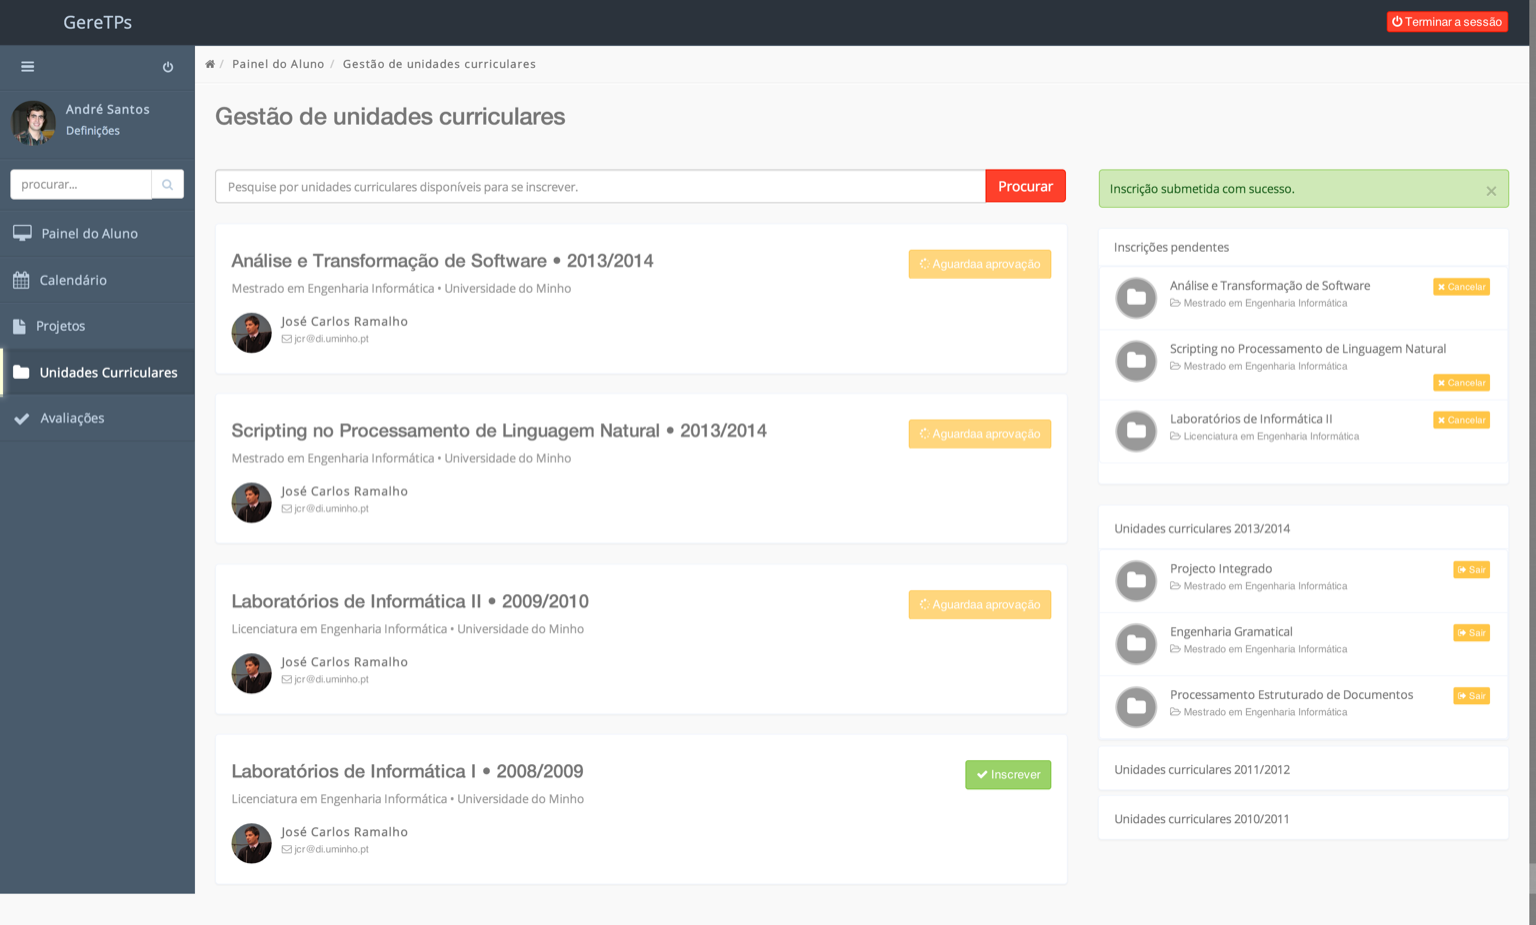
\includegraphics[width=1\textwidth,center]{images/implementacao/alunos/subjects}
  \caption{Página de gestão de unidades curriculares}
  \label{fig:student_subjects}
\end{figure}

\subsubsection{Gestão de avaliações}


\subsection{Painel do docente}

Nesta secção serão referidas todas as soluções já implementadas para o painel do docente.

Serão demonstradas todas as páginas e funcionalidades já implementadas para este tipo de utilizadores, com justificações para as decisões tomadas.

Um dos aspetos que se teve em atenção, no desenvolvimento do painel do docente foi a semelhança em relação ao painel do aluno. Ao haver uma semelhança entre os dois painéis, evita-se que o docente tenha a preocupação de verificar que a informação contida disponível é facilmente acedida pelos alunos.

Em todas as páginas, o docente terá acesso a um cabeçalho onde poderá voltar à página inicial, ao carregar no logótipo, ou terminar a sua sessão no botão mais à direita.

Para além do referido cabeçalho o docente terá acesso a uma barra lateral, onde poderá aceder às páginas de edição do perfil, página inicial do painel do docente, calendário, gestão projetos, gestão de unidades curriculares e gestão de avaliações.

O docente terá ainda acesso a uma barra de navegação que lhe permitirá saber sempre em que página do sistema se encontra, e voltar para páginas anteriores.

\subsubsection{Página inicial do painel do docente}
\label{ssub:teacher_dashboard}

Esta página é dirigida aos docentes autenticados, e é a primeira página que estes consultam após o registo ou autenticação.

Tal como foi referido na secção ~\ref{ssub:student_dashboard}, esta é a primeira página consultada e deve conter as ações mais importantes para um docente.
Além da listagem dos vários tipos de projetos, tal como acontece com os alunos, um docente tem acesso rápido à criação de um projeto (figura ~\ref{fig:teacher_project_new}).

\begin{figure}[H]
  \centering
  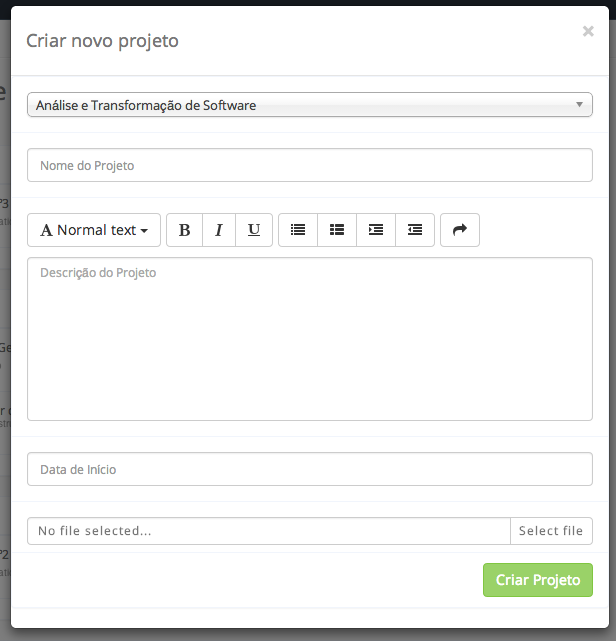
\includegraphics[width=1\textwidth,center]{images/implementacao/docentes/new_project}
  \caption{Novo projeto}
  \label{fig:teacher_project_new}
\end{figure}


Na Figura~\ref{fig:teacher_dashboard} pode ser consultada uma imagem demonstrativa da página desenvolvida.

\begin{figure}[H]
  \centering
  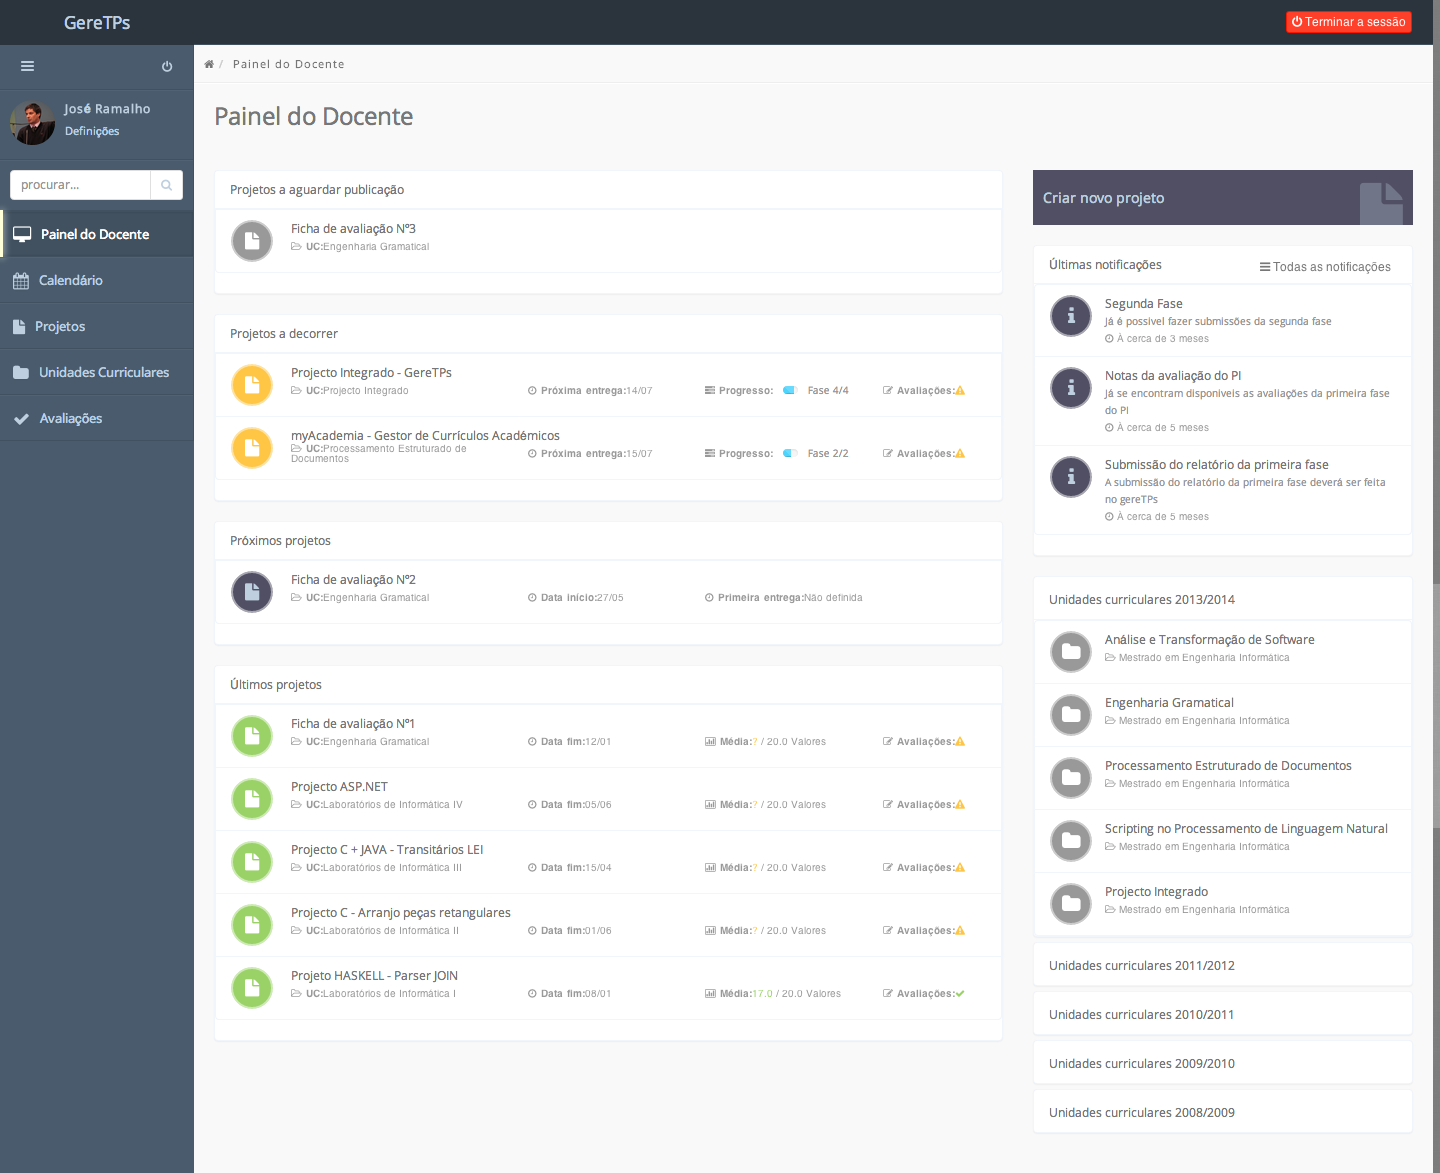
\includegraphics[width=1\textwidth,center]{images/implementacao/docentes/dashboard}
  \caption{Página inicial do painel do docente}
  \label{fig:teacher_dashboard}
\end{figure}

\subsubsection{Página de projeto}

É na página de projeto que um docente pode consultar todas as informações sobre um projeto de uma unidade curricular da qual faz parte.

Como foi descrito na secção ~\ref{ssub:student_project}, um projeto é uma das principais entidades do sistema e como tal teve-se o cuidado em garantir que o docente encontre a informação que necessita de uma forma simples e eficiente.

A diferença entre o conteúdo disponível entre a página de um projeto de um docente e de um aluno, são:

\begin{itemize}
	\item Edição de conteúdo do projeto sem necessidade de ser redirecionado para outra página
	\item Visualização e acesso as entregas efetuadas pelos alunos inscritos na unidade curricular em que o projeto de insere
	\item Ações de publicação e encerramento de um projeto
\end{itemize}

Na Figura~\ref{fig:teacher_project} pode ser consultada uma imagem demonstrativa da página desenvolvida.

\begin{figure}[H]
  \centering
  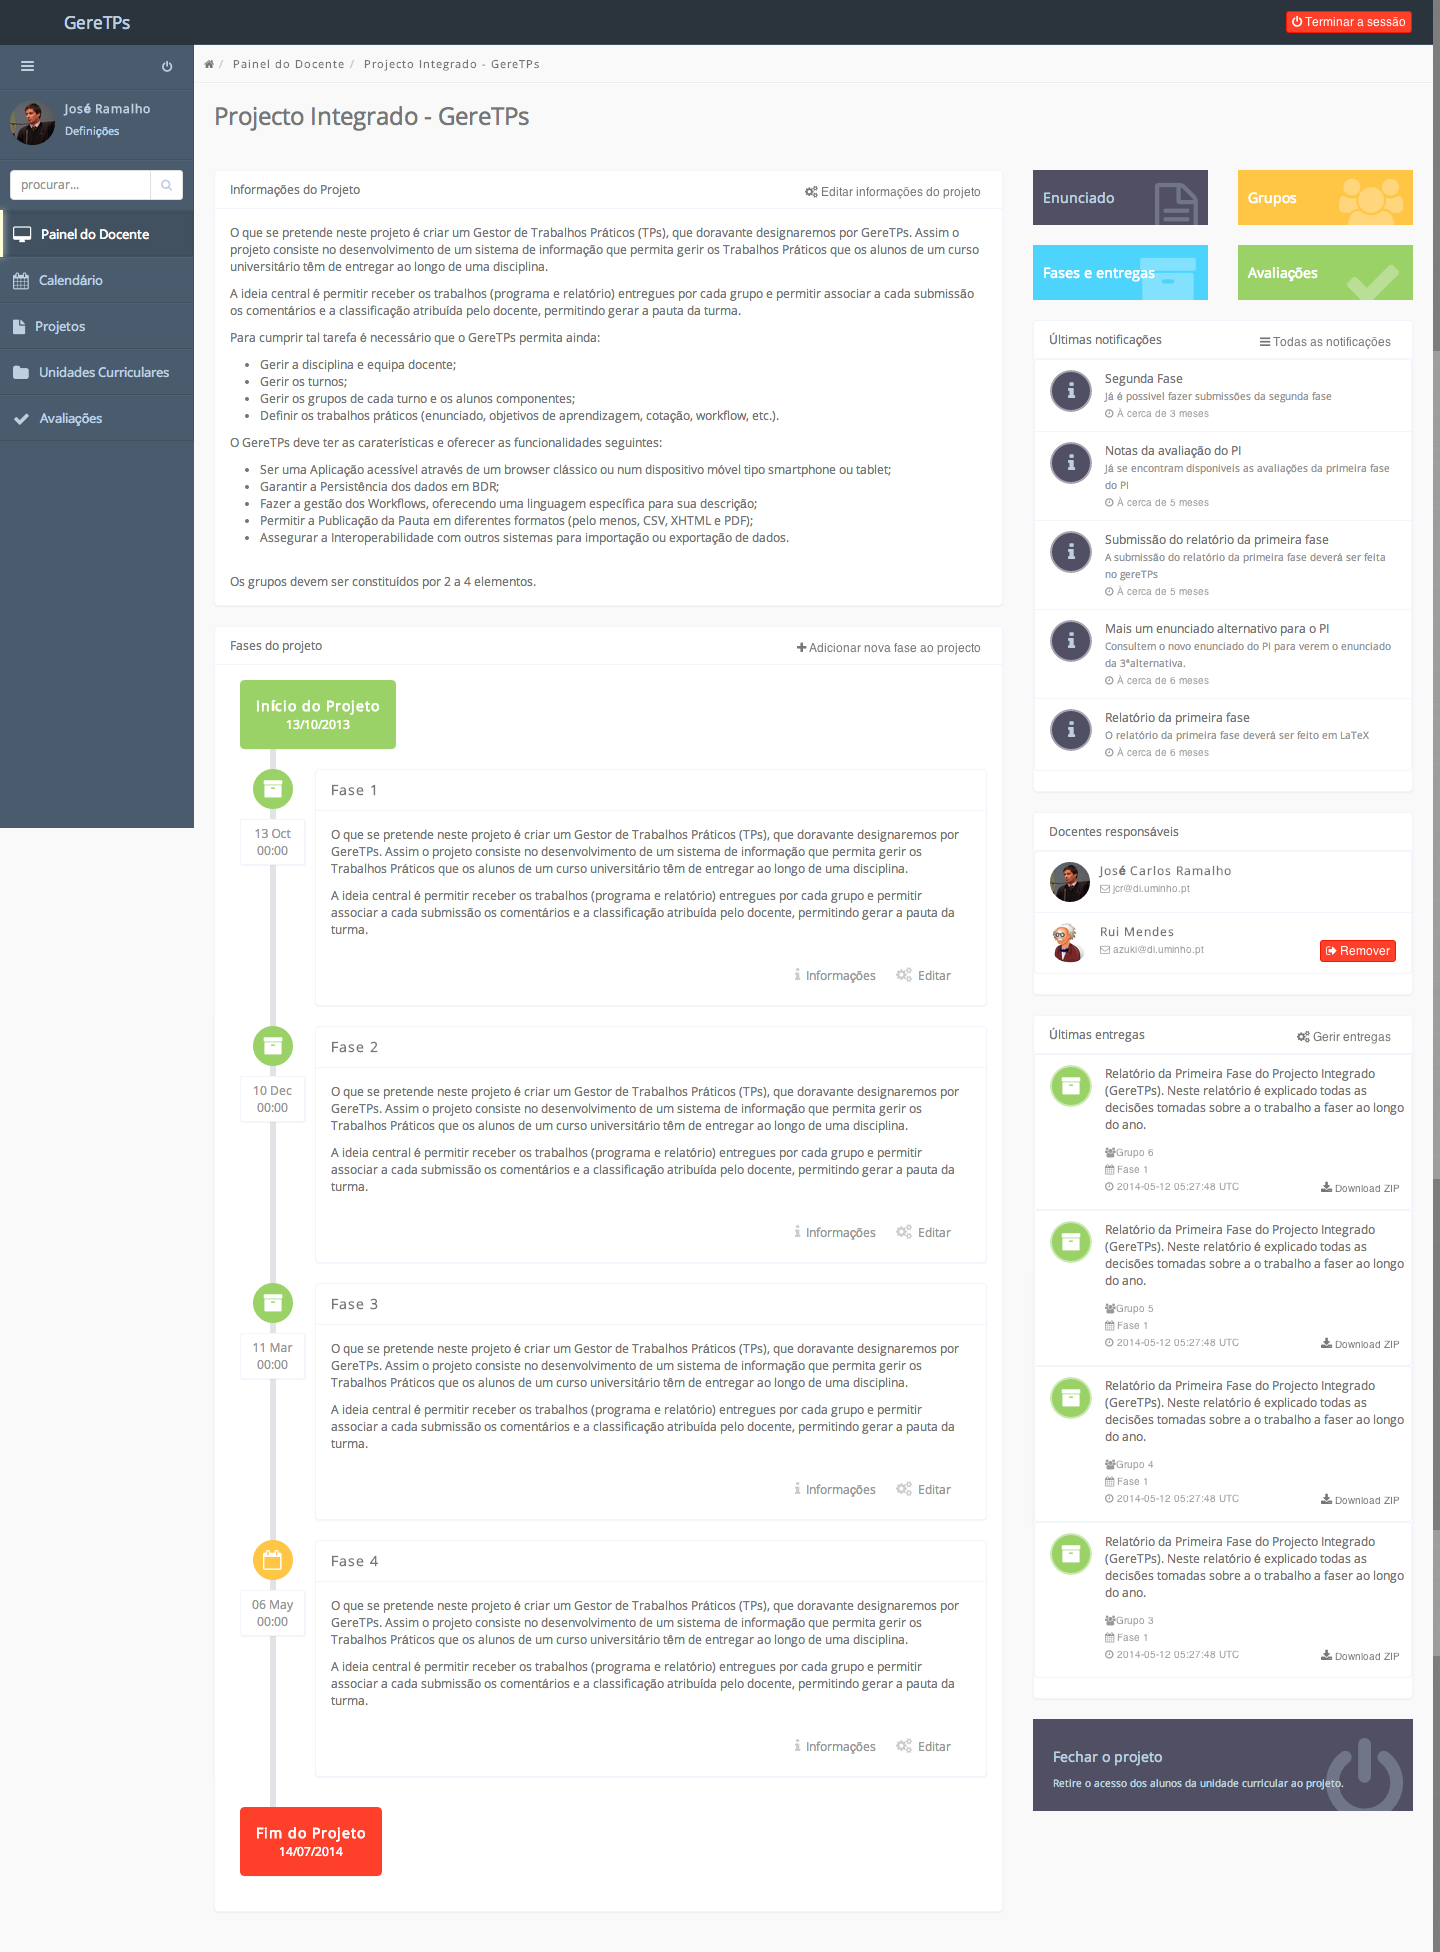
\includegraphics[width=.8\textwidth,center]{images/implementacao/docentes/project}
  \caption{Página de projeto}
  \label{fig:teacher_project}
\end{figure}

% \subsubsection{Gestão de grupos de trabalho}

\subsubsection{Gestão de fases e entregas}
\label{ssub:gestao_fases}

Na página dedicada à gestão de fases e entregas, um docente pode consultar e editar todas as informações das fases de um projeto, todas as entregas relativas às referidas fases.

Relativamente às fases, num plano principal, são apresentadas informações relativas às datas de inicio e de fim da fase, descrição, ficheiros de entrega obrigatória, ficheiros auxiliares, e atalhos para a pauta e para o enunciado da fase. Para cada fase, um docente pode consultar estatísticas, publicar a pauta e verificar quais os grupos que já efeturam entregas válidas.

Ao carregar numa entrega é possivel avaliar individualmente cada aluno. Para cada aluno, um docente pode deixar um comentário sobre a nota atribuída. Para auxiliar na da nota dada, o docente pode consultar resultados dos testes efetuados.

Na Figura~\ref{fig:teacher_deliveries} pode ser consultada uma imagem demonstrativa da página desenvolvida.

\begin{figure}[H]
  \centering
  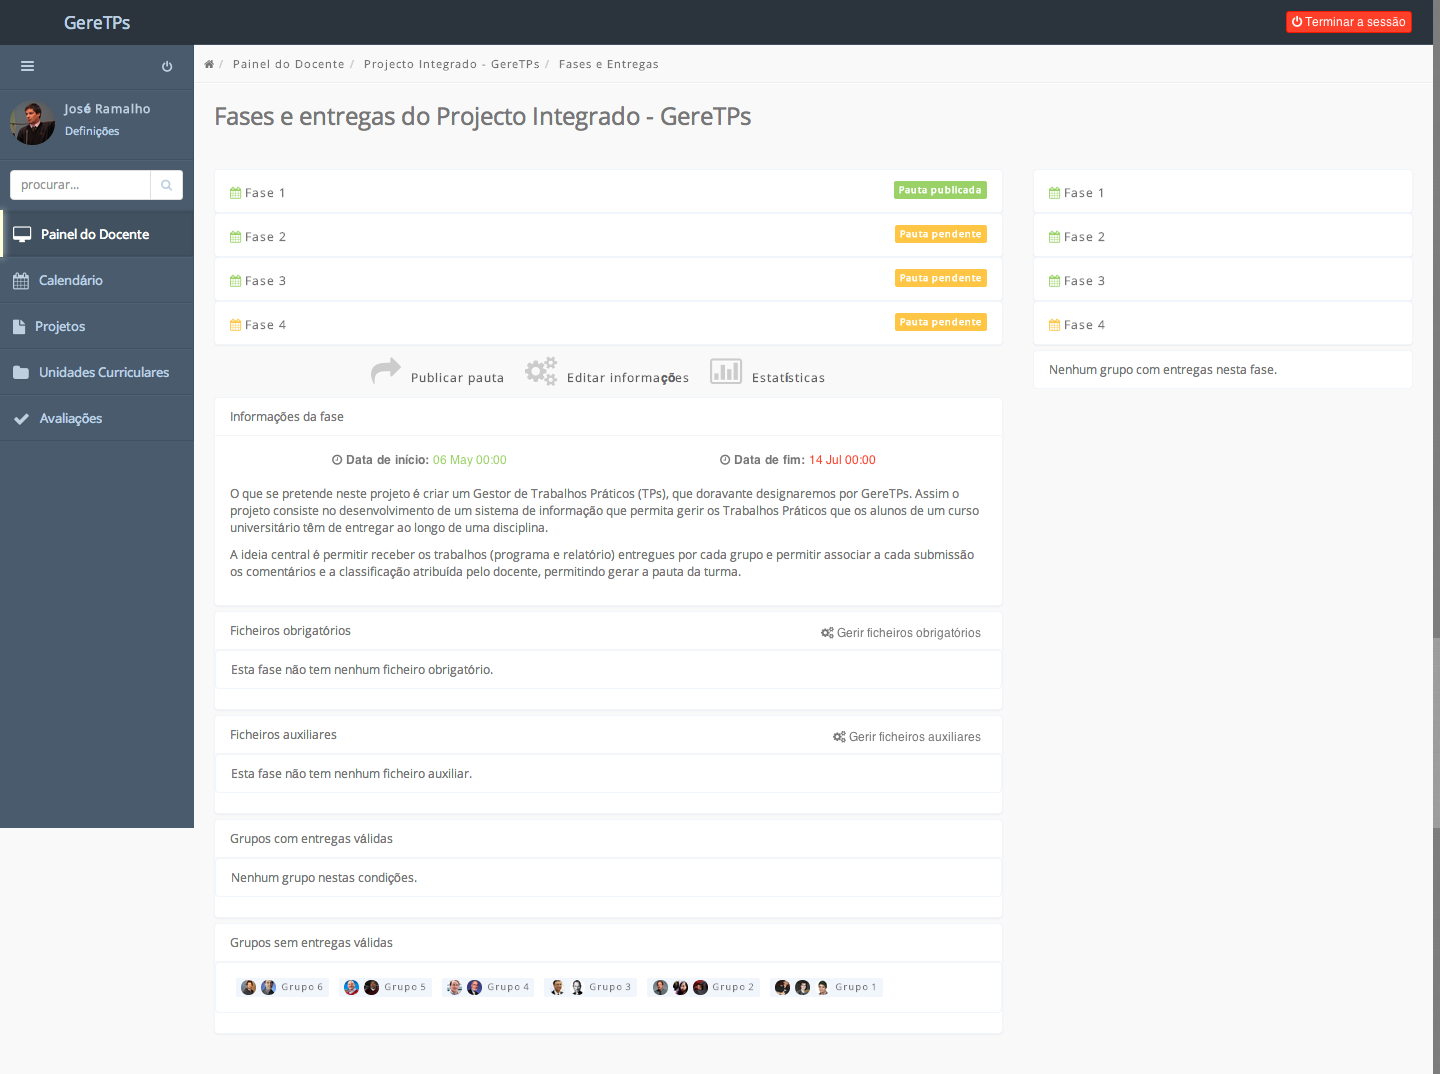
\includegraphics[width=1\textwidth,center]{images/implementacao/docentes/deliveries}
  \caption{Página de gestão de fases entregas}
  \label{fig:teacher_deliveries}
\end{figure}

% \subsubsection{Pautas de fase e projeto}

No página de gestão de um projeto, um aluno pode consultar uma pauta detalhada. Esta pauta lista todos os alunos inscritos na unidade curricular associada ao projeto e respetiva nota.

Além da nota final do projeto, também é possível ver a nota de cada fase.

Na Figura~\ref{fig:student_grades_project} pode ser consultada uma imagem demonstrativa da página desenvolvida.

\begin{figure}[H]
	\centering
	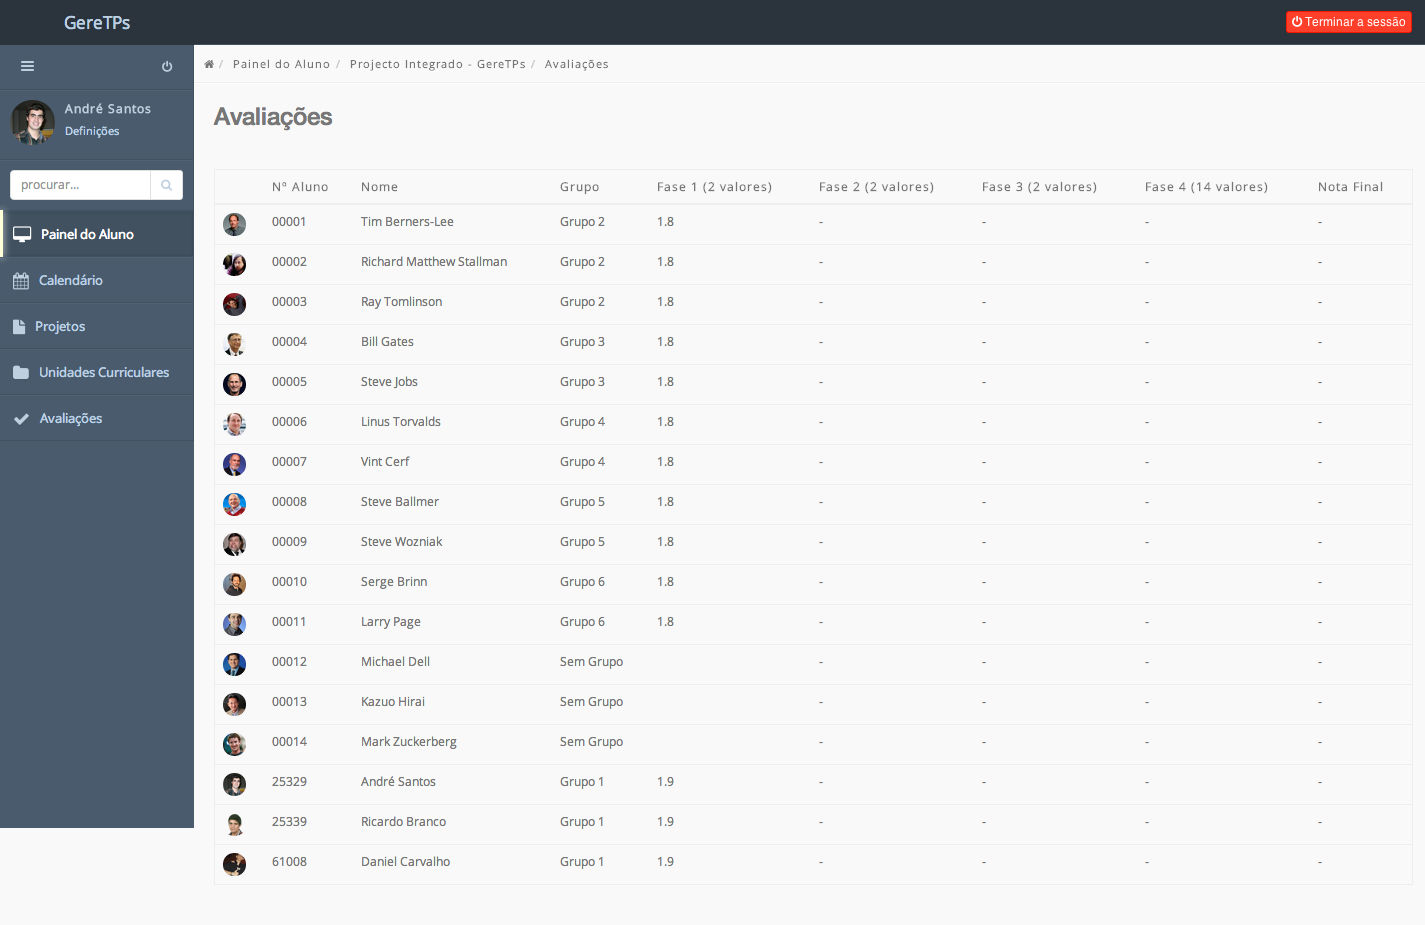
\includegraphics[width=1\textwidth,center]{images/implementacao/alunos/grades_project}
	\caption{Pauta de um projeto}
	\label{fig:student_grades_project}
\end{figure}

Ainda na página de gestão de um projeto, é possível aceder à página de \hyperref[ssub:gestao_fases]{Gestão de fases e entregas}. A partir desta página é possível um aluno consultar a pauta de uma fase de um projeto, caso esta já tenha sido lançada por um dos docentes da unidade curricular associada ao projeto.

A pauta de uma fase é bastante semelhante à pauta de um projeto, com a particularidade de esta apresentar a nota da fase entre zero e vinte valores e a nota correspondente no final do projeto.

Na Figura~\ref{fig:student_grades_phase} pode ser consultada uma imagem demonstrativa da página desenvolvida.

\begin{figure}[H]
	\centering
	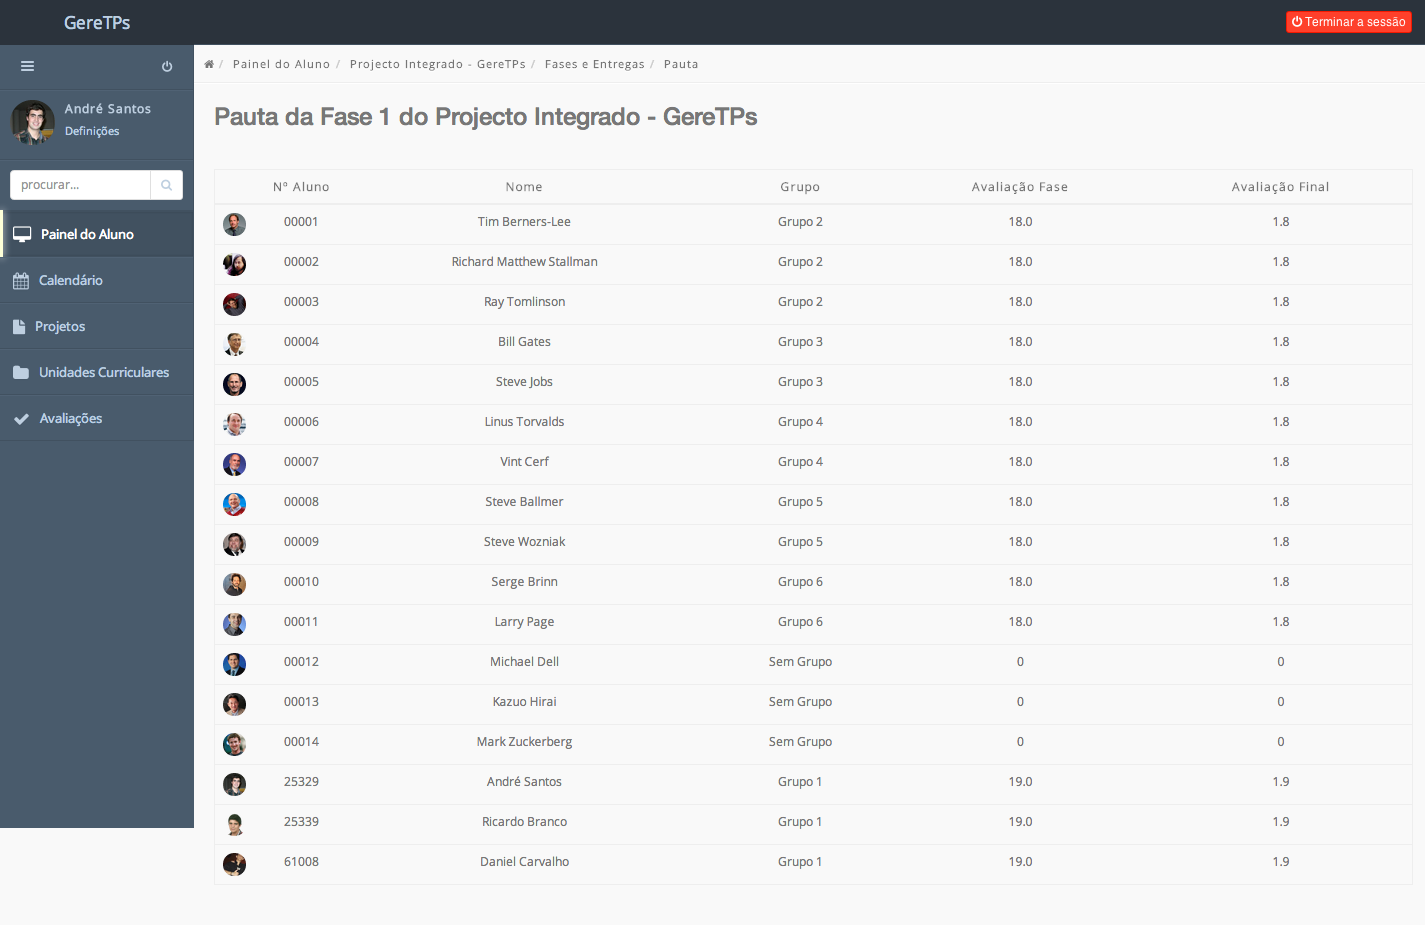
\includegraphics[width=1\textwidth,center]{images/implementacao/alunos/grades_phase}
	\caption{Pauta da uma fase}
	\label{fig:student_grades_phase}
\end{figure}

 \subsubsection{Gestão de unidades curriculares}

Na pagina de gestão de unidades curriculares, um docente pode consultar todas as unidades curriculares em que este está inserido (figura ~\ref{fig:teacher_ucs_index}) e criar uma nova unidade curricular (figura ~\ref{fig:teacher_new_uc}).


\begin{figure}[H]
  \centering
  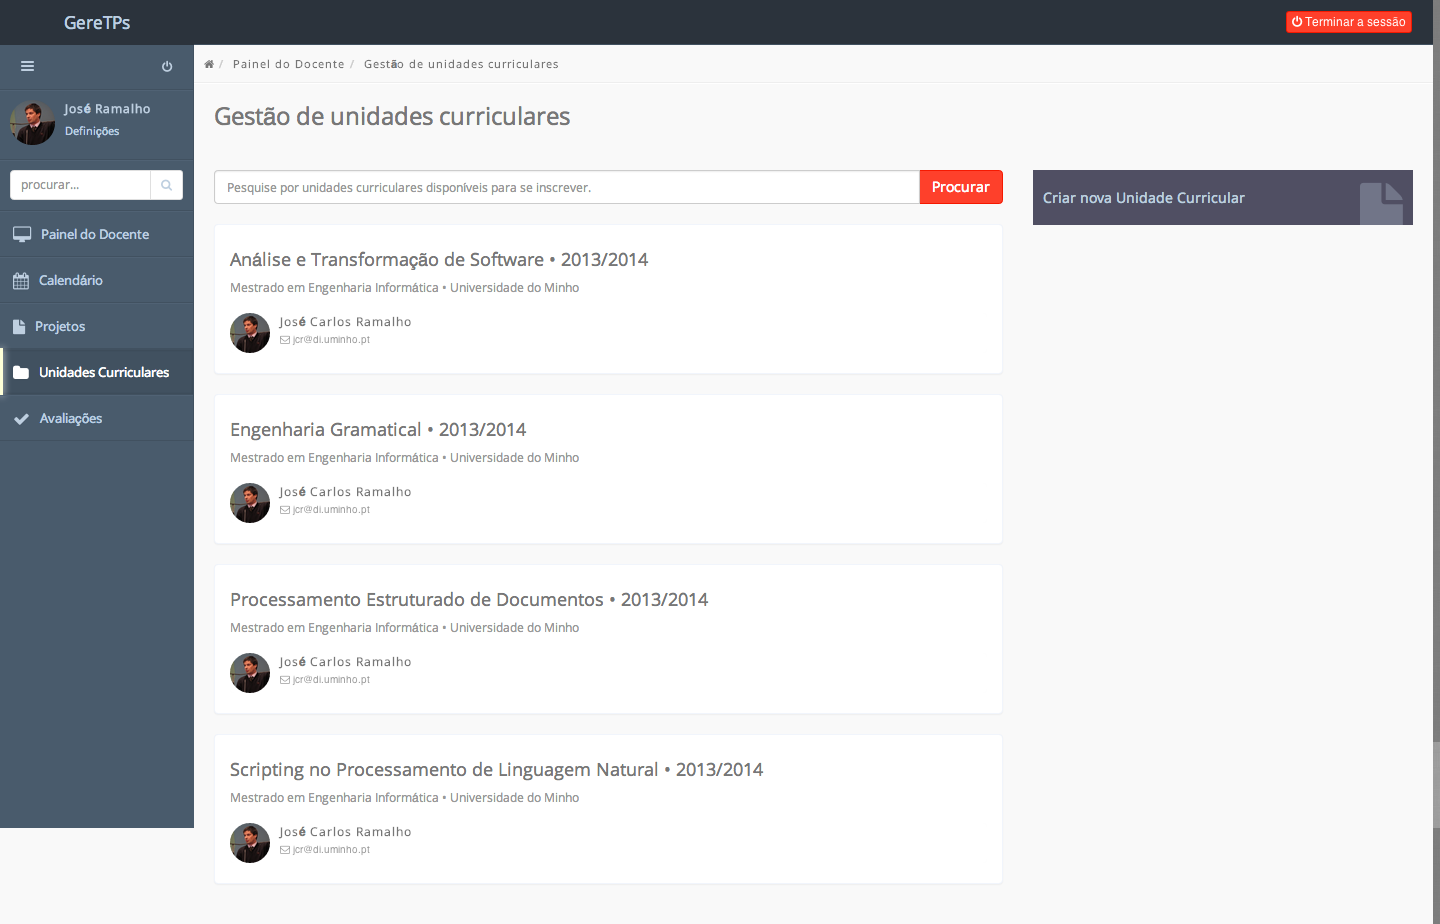
\includegraphics[width=1\textwidth,center]{images/implementacao/docentes/ucs_index}
  \caption{Página de gestão de unidades curriculares}
  \label{fig:teacher_ucs_index}
\end{figure}

\begin{figure}[H]
  \centering
  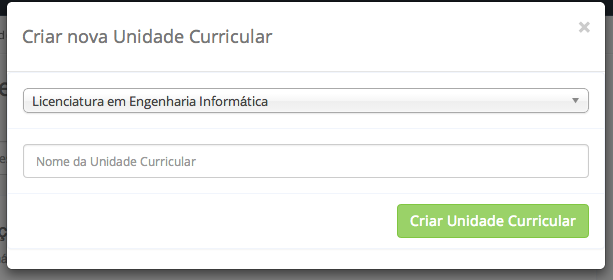
\includegraphics[width=1\textwidth,center]{images/implementacao/docentes/new_uc}
  \caption{Nova Unidade Curricular}
  \label{fig:teacher_new_uc}
\end{figure}

Após criar uma nova unidade curricular, o docente é reencaminhado para a página da unidade curricular criada.

Na página de uma unidade curricular é possível visualizar os projetos dessa unidade curricular, adicionar docentes e fazer gestão de alunos e turnos.

Na página de gestão de alunos (figura ~\ref{fig:uc_students}), um docente pode aceitar ou remover a inscrição de um aluno.

\begin{figure}[H]
  \centering
  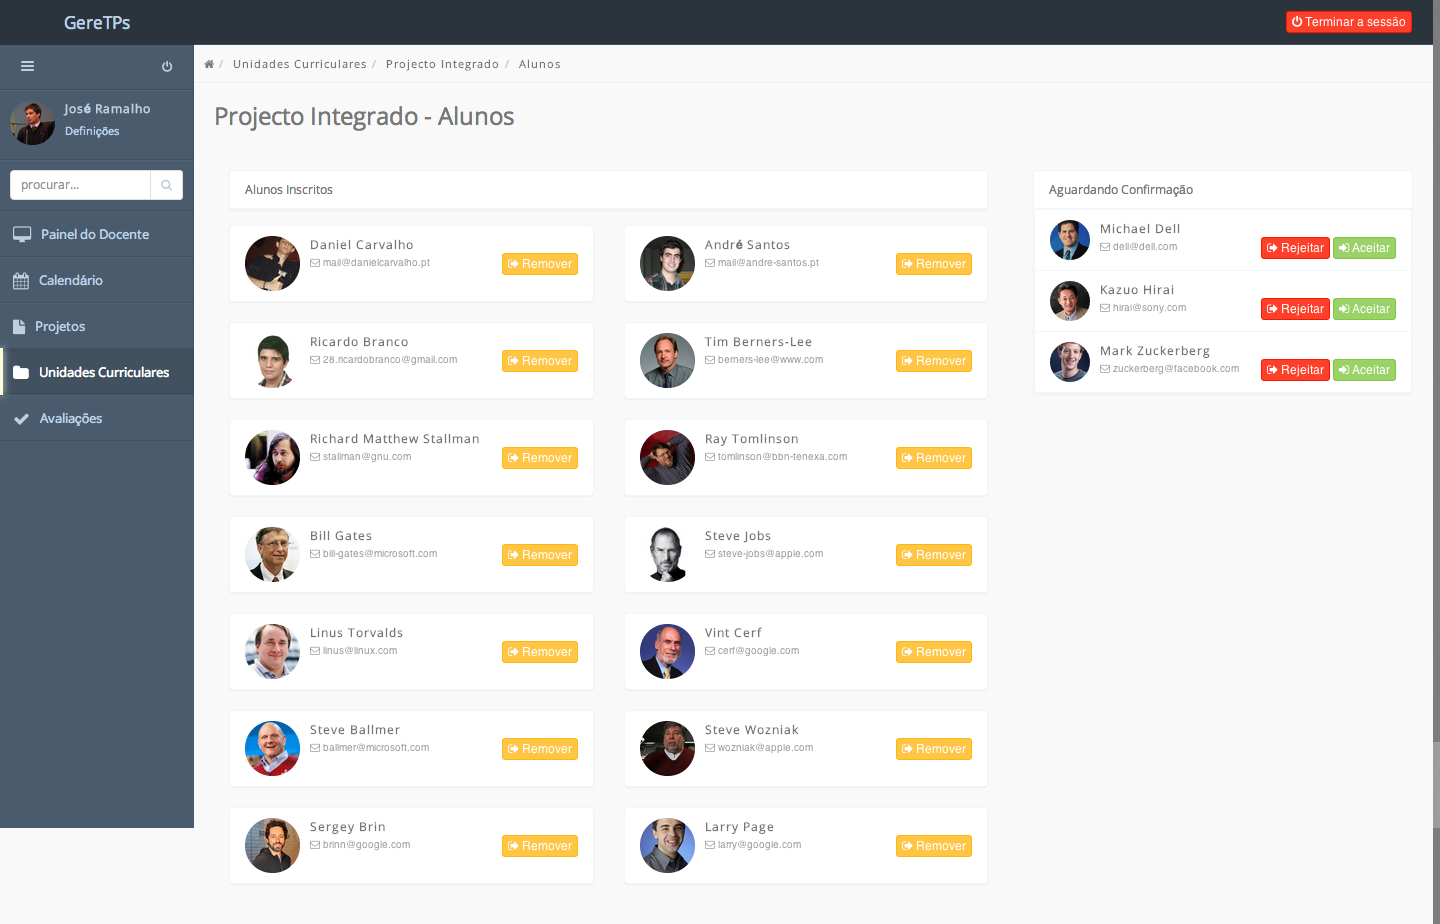
\includegraphics[width=1\textwidth,center]{images/implementacao/docentes/uc_students}
  \caption{Gestão de alunos de uma unidade curricular}
  \label{fig:uc_students}
\end{figure}


Na página de gestão de alunos (figura ~\ref{fig:uc_shifts}), um docente pode criar turnos e adicionar ou remover um aluno de um turno.

\begin{figure}[H]
  \centering
  \includegraphics[width=1\textwidth,center]{images/implementacao/docentes/uc_shifts}
  \caption{Gestão de turnos de uma unidade curricular}
  \label{fig:uc_shifts}
\end{figure}


Na Figura~\ref{fig:teacher_subjects} pode ser consultada uma imagem demonstrativa da página desenvolvida.

\begin{figure}[H]
  \centering
  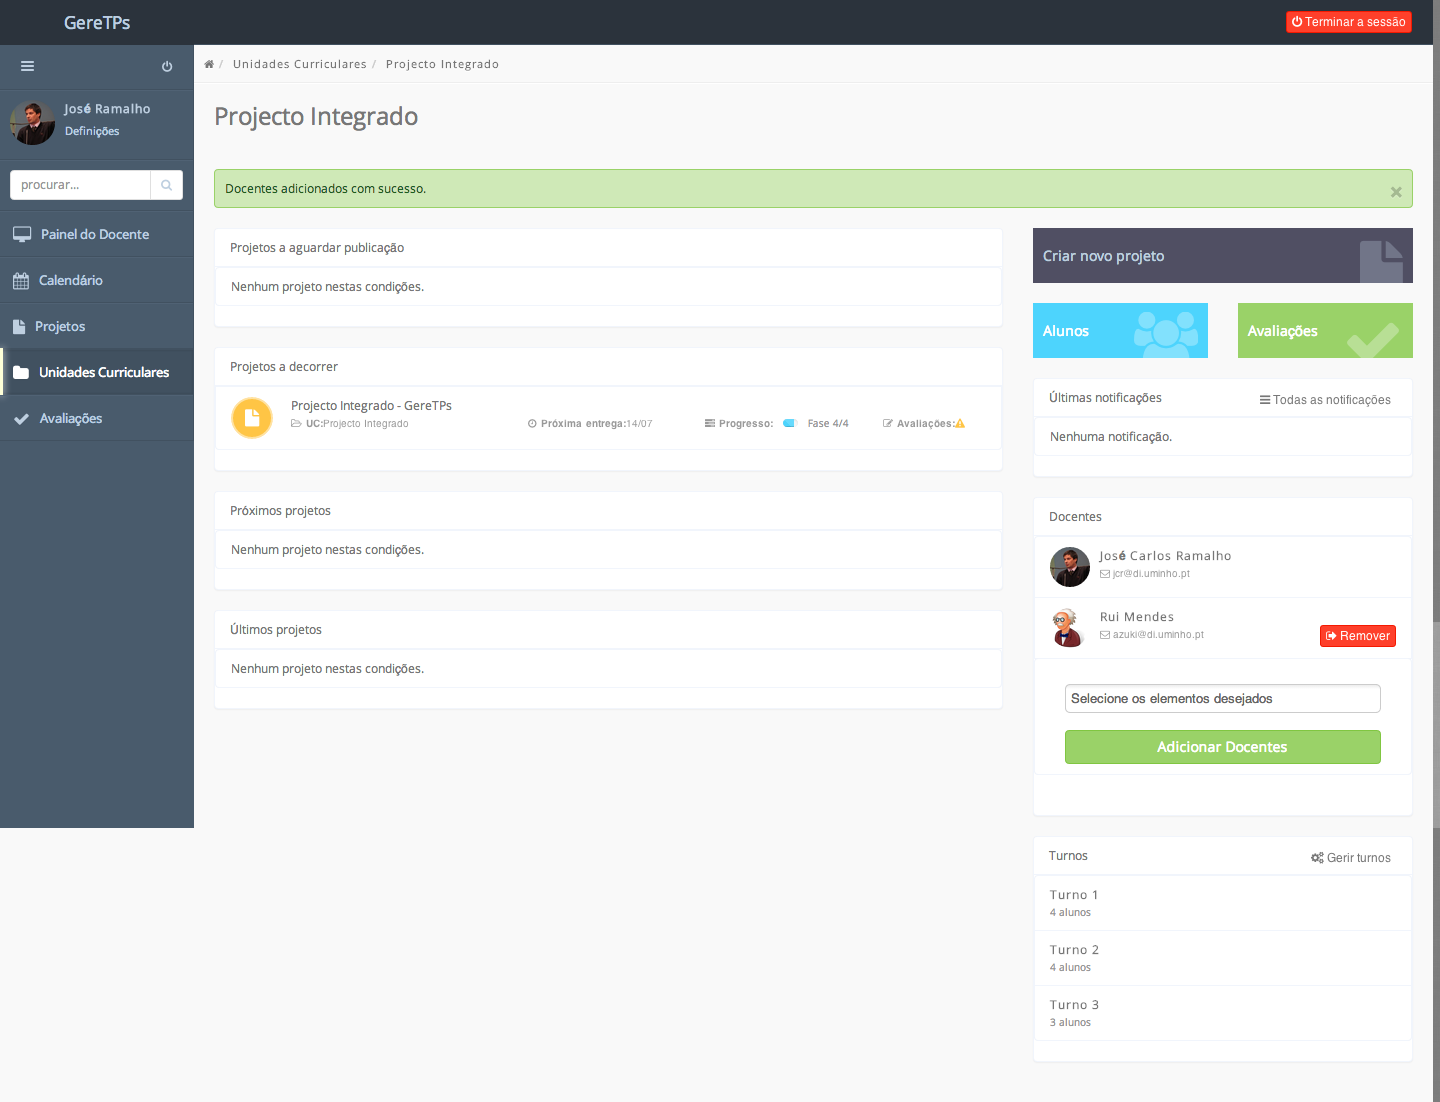
\includegraphics[width=1\textwidth,center]{images/implementacao/docentes/uc}
  \caption{Página de uma unidade curricular}
  \label{fig:teacher_subjects}
\end{figure}

 \subsubsection{Testes} % (fold)
\label{ssub:testes}

Quando uma fase ainda se encontra aberta para submissões, o docente pode adicionar testes que permitem ajudar o mesmo no processo de avaliação. Estes testes são executados quando um aluno faz uma submissão.

Na Figura~\ref{fig:tests} pode ser consultada uma imagem demonstrativa da página desenvolvida.

\begin{figure}[H]
  \centering
  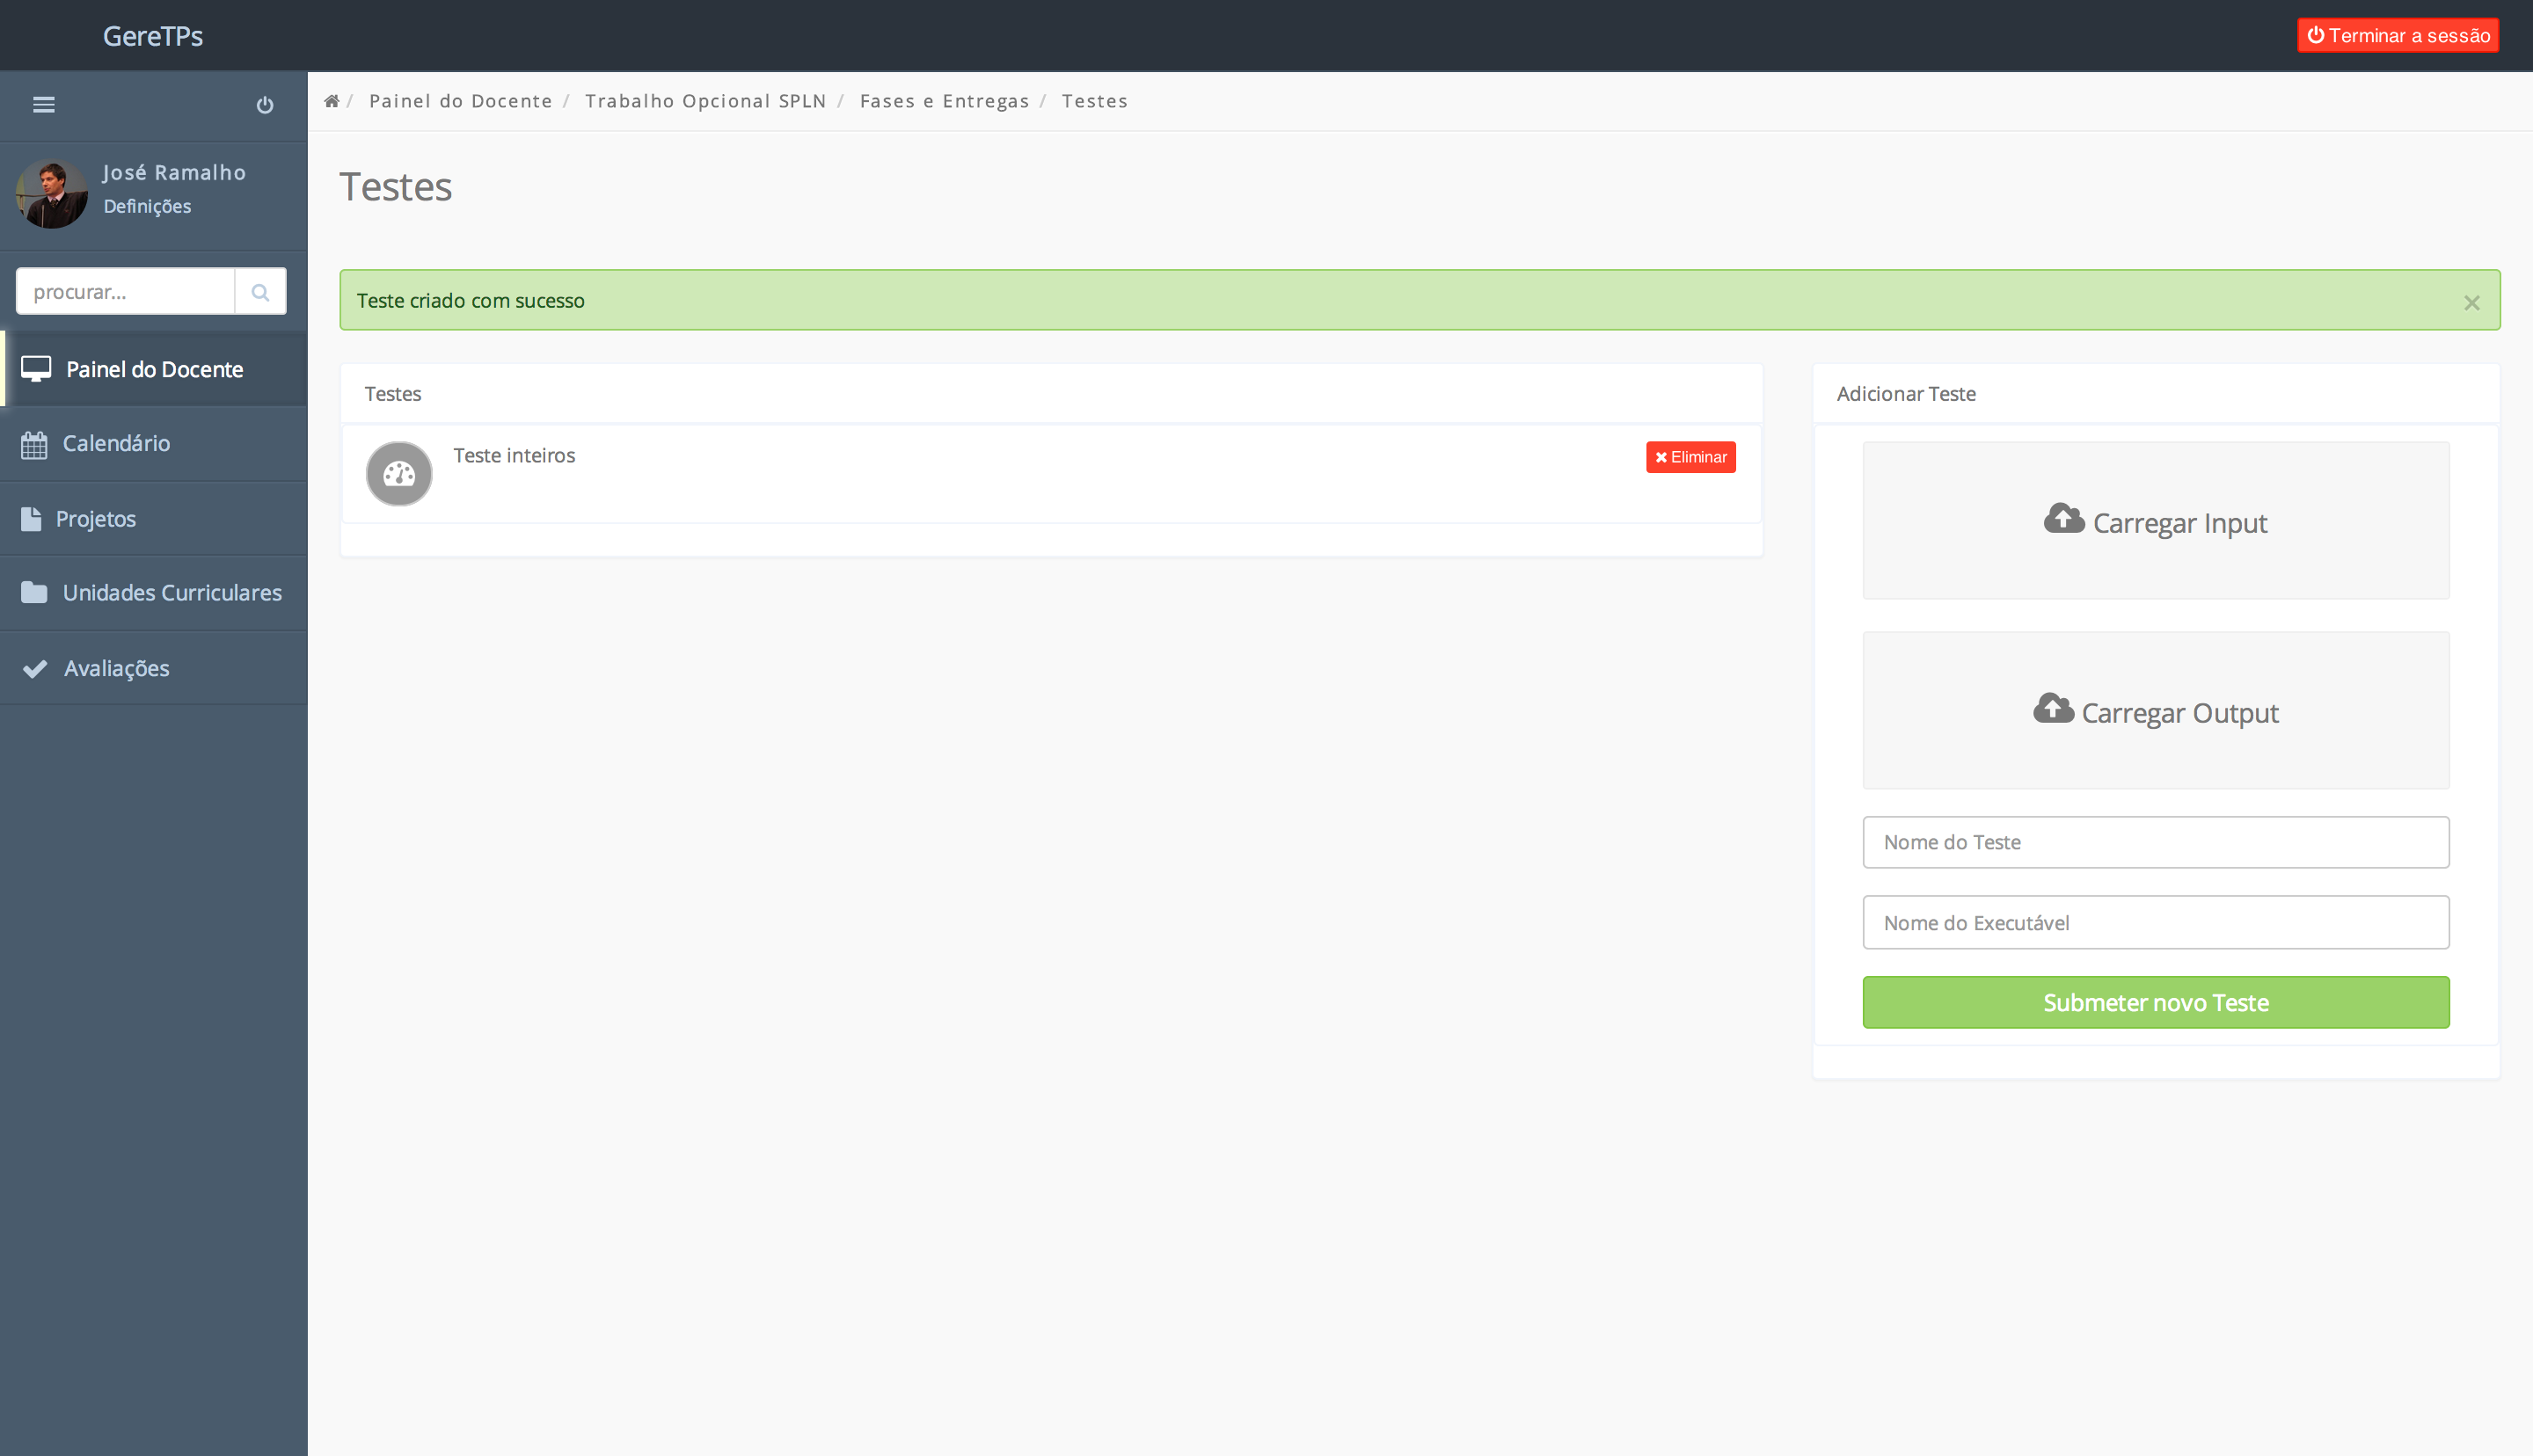
\includegraphics[width=.8\textwidth,center]{images/implementacao/docentes/testes}
  \caption{Página de criação de testes}
  \label{fig:tests}
\end{figure}

% subsubsection testes (end)

 \subsubsection{Consulta e avaliação de uma entrega}
\label{ssub:entrega_avaliacao}

Ao carregar numa entrega, o utilizador é direcionado para uma página onde pode consultar as informações da referida entrega, assim como proceder à sua avaliação.\\

Nesta página o utilizador pode consultar a descrição da entrega, fazer download dos ficheiros que a constituem e consultar os resultados dos testes a que a entrega foi submetida.\\

Pode também facilmente avaliar os alunos que constituem o grupo que efetuou a entrega, indicando a sua avaliação e uma nota auxiliar.\\

Na Figura~\ref{fig:delivery_grades} pode ser consultada uma imagem demonstrativa da página desenvolvida.

\begin{figure}[H]
  \centering
  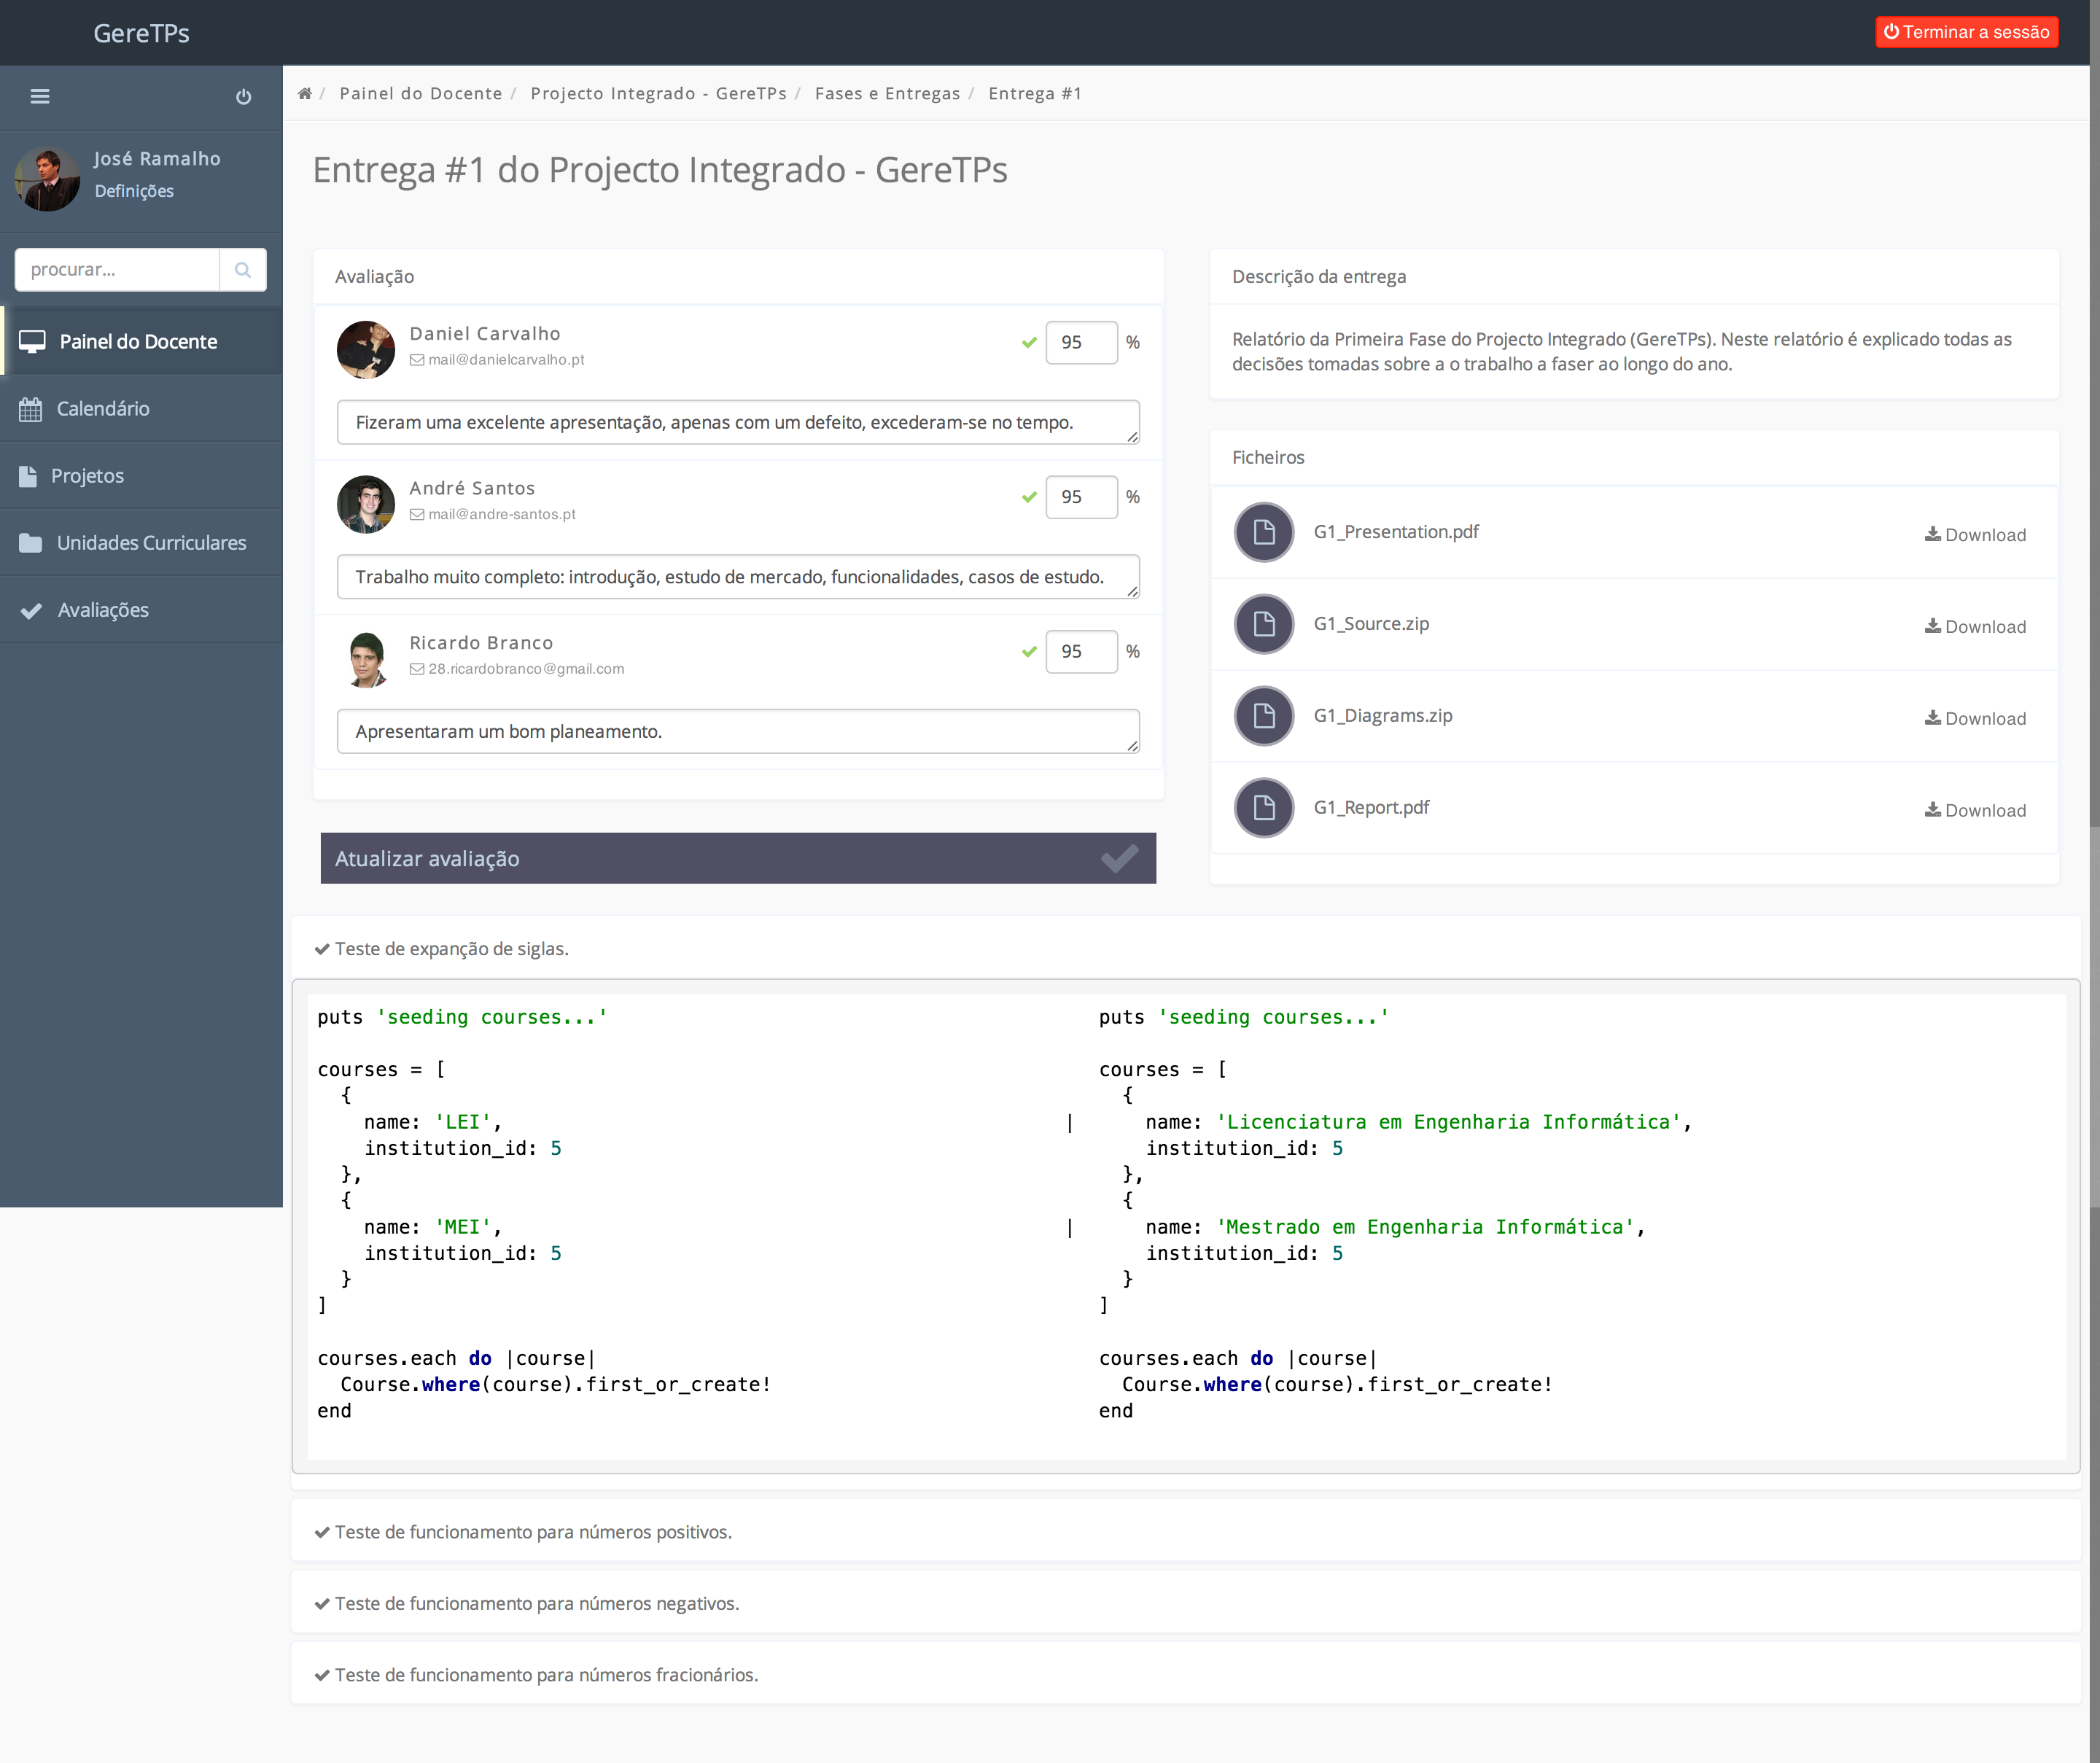
\includegraphics[width=1\textwidth,center]{images/implementacao/docentes/delivery_and_grades}
  \caption{Página de consulta e avaliação de uma entrega}
  \label{fig:delivery_grades}
\end{figure}



\subsection{Sistema de notificações}

Um das informações disponibilizadas na página inicial de um utilizador registado são as notificações. Estas têm como objetivo informar o utilizador quais foram as atividades exercidas por outros utilizadores.

Por exemplo, para um docente, é importante que haja uma notificação, sempre que um aluno faz uma entrega num projeto. Assim evita-se que o docente esteja sempre a aceder à página de entregas para verificar se houveram novas alterações.

No caso dos alunos, é importante saber que um docente lançou no sistema um novo projeto, que houveram alterações no enunciado de uma fase, ou que um elemento de um dos seus grupos submeteu uma entrega.

Uma notificação está sempre associada a um projeto, portanto quando se carrega numa notificação o utilizador é redirecionado para a página do projeto respetivo.

Recorrendo às suas notificações, evita-se que um utilizador tenha que percorrer a aplicação por completo com o objetivo de verificar se ocorreram alterações no sistema.

Na página de um projeto, também são disponibilizadas notificações. Estas possuem as mesmas características das notificações existentes na página inicial.

Na Figura~\ref{fig:notifications} pode ser consultada uma imagem demonstrativa da funcionalidade implementada.

\begin{figure}[H]
  \centering
  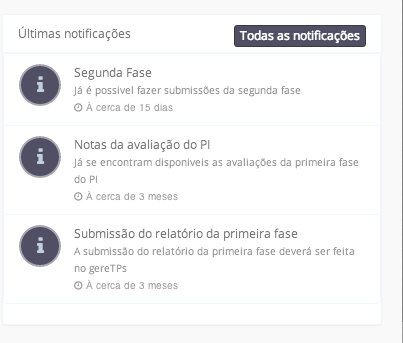
\includegraphics[width=0.65\textwidth,center]{images/implementacao/alunos/notifications}
  \caption{Notificações}
  \label{fig:notifications}
\end{figure}

\subsection{Sistema de emails}

Além das notificações da aplicação, um utilizador também pode ser notificado através de \texit{email}.

Uma das grandes vantagens dos emails em relação às notificações é que o utilizador não precisa de aceder à aplicação para saber dos eventos mais importantes.

Algumas das situações em que um sistema de \texit{email} se torna  vantajoso são:

\begin{itemize}
	\item Submissão de uma entrega
	\item Lançamento de notas
	\item Inscrição numa unidade curricular
	\item Admissão num grupo
	\item Novo projeto
	\item Aproximação do final de uma fase
\end{itemize}

No caso da submissão de uma entrega, todos os elementos do grupo serão notificados com um \texit{email} com a descrição da submissão e com \texit{links} para os ficheiros submetidos. Neste caso o email pode ser importante como comprovativo da entrega.

Na figura ~\ref{fig:mail} é possível ver o conteúdo de um \texit{email} que foi recebido após a submissão de uma entrega.

\begin{figure}[H]
	\centering
	
\includegraphics[width=0.65\textwidth,center]{images/implementacao/alunos/emails}
	\caption{Notificações}
	\label{fig:mail}
\end{figure}

\subsection{Exportações em JSON}

Uma das funcionalidades implementadas é a capacidade de responder a pedidos \textit{JSON}. Desta forma permite-se que outras aplicações externas possam comunicar com esta aplicação, sem ter conhecimento da implementação da mesma e garantido interoperabilidade.

Ao exportar a aplicação numa linguagem como \textit{JSON}, torna-se possível fazer \textit{parsing} de uma linguagem bem estruturada e normalizada e que não esta obstruida com elementos de \textit{layout}.\\

Nos exemplos seguintes, pode-se verificar as respostas à dois pedido \textit{JSON} que pertendem obter a lista de todas as unidades curriculares do sistema, e informações sobre uma unica unidade curricular

\begin{spverbatim}
	Pedido:
	domain/subjects.json

	Resposta:
	[{"id":5,"name":"Projecto Integrado","course_id":2,
	"responsible_id":1,"academic_year_id":5},
	{"id":1,"name":"Análise e Transformação de Software","course_id":2,
	"responsible_id":1,"academic_year_id":5},
	{"id":2,"name":"Engenharia Gramatical","course_id":2,
	"responsible_id":1,"academic_year_id":5},
	{"id":3,"name":"Processamento Estruturado de Documentos","course_id":2,
	"responsible_id":1,"academic_year_id":5},
	{"id":4,"name":"Scripting no Processamento de Linguagem Natural","course_id":2,
	"responsible_id":1,"academic_year_id":5},
	{"id":6,"name":"Laboratórios de Informática IV","course_id":1,
	"responsible_id":1,"academic_year_id":4},
	{"id":7,"name":"Laboratórios de Informática III","course_id":1,
	"responsible_id":1,"academic_year_id":3},
	{"id":8,"name":"Laboratórios de Informática II","course_id":1,
	"responsible_id":1,"academic_year_id":2},
	{"id":9,"name":"Laboratórios de Informática I","course_id":1,
	"responsible_id":1,"academic_year_id":1}]
\end{spverbatim}

\begin{spverbatim}
	Pedido:
	domain/subjects/1.json

	Resposta:
	{"id":1,"name":"Análise e Transformação de Software","course_id":2,
	"responsible_id":1,"academic_year_id":5}
\end{spverbatim}

\subsection{Sistema adaptado a todos os dispositivos}
Hoje em dia, o acesso à aplicações \textwidth{web} através de dispositivos móveis é cada vez maior.

A garantia de uma maior experiência de visualização, fácil leitura e a redução do redimensionamento do conteúdo da aplicação são fatores que contribuem para o sucesso da mesma.

Esses mesmos fatores foram tidos em consideração nesta aplicação, garantindo que esta está preparada para ser acedida em dispositivos de diferentes resoluções.

Nas imagens seguintes são representadas algumas das principais páginas da aplicação quando visionadas em ecrãs de menor resolução:

\begin{figure}[H]
	\centering
 	
\includegraphics[width=0.65\textwidth,center]{images/implementacao/alunos/home}
 	\caption{Página Inicial}
 	\label{fig:home_smal}
 \end{figure}

\begin{figure}[H]
	\centering
	\begin{subfigure}{0.5\textwidth}
 		\centering
 		\includegraphics[width=0.95\textwidth,center]{images/implementacao/alunos/dashboard_small}
 		\subcaption{Painel do aluno}
 		\label{fig:dashboard_small}
 	\end{subfigure}
 	\begin{subfigure}{0.55\textwidth}
	 	\centering
	 	\includegraphics[width=0.95\textwidth,center]{images/implementacao/alunos/ucs}
	 	\subcaption{Gestão de unidades curriculares}
	 	\label{fig:ucs_small}
 	\end{subfigure}
 \end{figure}


 \begin{figure}[H]
	\centering
	\begin{subfigure}{0.45\textwidth}
 		\centering
 		\includegraphics[width=0.95\textwidth]{images/implementacao/alunos/project_small}
 		\subcaption{Página de um projeto}
 		\label{fig:project_small}
 	\end{subfigure}
 	\begin{subfigure}{0.45\textwidth}
 		\centering
 		\includegraphics[width=0.95\textwidth]{images/implementacao/alunos/entrega}
 		\subcaption{Entrega de uma fase}
 		\label{fig:delivery_small}
 	\end{subfigure}
 \end{figure}





\subsection{GereTPS REST API}

Com o objetivo de garantir que o sistema seja facilmente integrável com outras ferramentas e sistemas, foi desenvolvida uma \textit{API} que segue todos os princípios \textit{REST}.\\

Nesta fase do projeto a API está a responder aos métodos \textit{show}, que dado um determinado \textit{id} responde com todas as informações desse objeto, e \textit{index} que lista informações de todos os objetos do tipo requerido.\\

No acesso a informação privada, o utilizador necessita de indicar o seu email e o \textit{token} de autenticação que pode ser obtido ao criar uma sessão.

Na implementação da API, foram tidos todos os cuidados para que o utilizador apenas aceda a informação que lhe seja relativa. \\

Até ao momento a API responde aos seguintes pedidos:

\begin{itemize}
  \item POST \verb%/sessions% \\ Devolve as informações de autenticação para o utilizador.
  \item GET \verb%/projects% \\ Devolve todas os projetos em que o utilizador está envolvido.
  \item GET \verb%/projects/:id% \\ Devolve todas as informações do projeto indicado.
  \item GET \verb%/phases% \\ Devolve todas as fases em que o utilizador está envolvido.
  \item GET \verb%/phases/:id% \\ Devolve todas as informações da fase indicada.
  \item GET \verb%/projects/:project_id/phases% \\ Devolve todas as fases do projeto indicado em que o utilizador está envolvido
  \item GET \verb%/groups% \\ Devolve todos os grupos dos projetos em que o utilizador está envolvido.
  \item GET \verb%/groups/:id% \\ Devolve todas as informações do grupo indicado.
  \item GET \verb%/projects/:project_id/groups% \\ Devolve todos os grupos do projeto indicado em que o utilizador está envolvido.
  \item GET \verb%/phases/:phase_id/groups% \\ Devolve todos os grupos da fase indicada em que o utilizador está envolvido.

  \item GET \verb%/deliveries% \\ Devolve todas as entregas dos projetos em que o utilizador está envolvido.
  \item GET \verb%/deliveries/:id% \\ Devolve todas as informações da entrega indicada.
  \item GET \verb%/phases/:phase_id/deliveries% \\ Devolve todas as entregas da fase indicada em que o utilizador está envolvido.
  \item GET \verb%/phases/:phase_id/groups/:group_id/deliveries% \\ Devolve todas as entregas da fase indicada, efetuadas pelo grupo com o \textit{id} especificado.

  \item GET \verb%/documents% \\ Devolve todos os documentos das entregas em que o utilizador está envolvido.
  \item GET \verb%/documents/:id% \\ Devolve todas as informações do documento indicado.
  \item GET \verb%/deliveries/:delivery_id/documents% \\ Devolve todos os documentos da entrega indicada em que o utilizador está envolvido.

  \item GET \verb%/documents/:id/download% \\ Devolve o documento especificado.
\end{itemize}

A \textit{API} por omissão responde em formato \textit{JSON}, no entanto se o pedido for efetuado com a extensão \textit{XML}, os pedidos são devolvidos nesse mesmo formato.

\subsection{Interface PERL para a API do sistema}

Para facilitar a utilização da API do sistema, foi desenvolvida uma interface em PERL que permite comunicar com o sistema de uma forma mais simples.

Pretende-se assim facilitar o desenvolvimento de ferramentas que comuniquem com o sistema.\\

A referida interface foi desenvolvida recorrendo a vários módulos PERL, que são descritos de seguida:

\begin{itemize}
  \item \verb%Net::GereTPs% \\ Módulo responsável por reencaminhar o acesso para a versão correta da API.
  \item \verb%NET::GereTPs::V1% \\ Módulo responsável por reencaminhar os pedidos para os módulos respetivos, e armazenar as informações de autenticação.
  \item \verb%NET::GereTPs::V1::Session% \\ Módulo responsável pelos pedidos de autenticação.
  \item \verb%NET::GereTPs::V1::Projects% \\ Módulo responsável pelos pedidos ao controlador de projetos do sistema.
  \item \verb%NET::GereTPs::V1::Phases% \\ Módulo responsável pelos pedidos ao controlador de fases do sistema.
  \item \verb%NET::GereTPs::V1::Deliveries% \\ Módulo responsável pelos pedidos ao controlador de entregas do sistema.
  \item \verb%NET::GereTPs::V1::Documents% \\ Módulo responsável pelos pedidos ao controlador de documentos do sistema.
  \item \verb%NET::GereTPs::V1::Groups% \\ Módulo responsável pelos pedidos ao controlador de grupos do sistema.
\end{itemize}

De seguida pode consultar-se um exemplo de utilização da interface desenvolvida:

\begin{verbatim}
use Net::GereTPs;

my $geretps = Net::GereTPs->new({email => $params{email}, password => $params{password}});
my $auth_token = $geretps->session->get_auth_token();
my $projects = $geretps->projects->all();
my $group_info = $geretps->groups->get_xml($group_id);
my $groups = $geretps->groups("phases",$phase_id)->all();
\end{verbatim}

\subsection{Utilitário de linha de comandos}

O principal objetivo do sistema é facilitar ao máximo a gestão de alunos, trabalhos práticos e avaliações por parte do utilizador. \\

Para facilitar a realização de algumas tarefas e melhorar o desempenho dos utilizadores avançados do sistema, foi desenvolvido um utilitário de linha de comandos que permite realizar várias ações importantes do sistema de forma mais rápida e eficiente.

Segue-se o menu de ajuda do utilitário onde estão descritas as funcionalidades implementadas na versão atual:

\begin{verbatim}
SAGE: geretps <command> [<args>]

Commands:
  init                                Create an empty geretps folder or reinitialize an existing one.
  login -E <email> -P <password>      Get authentication token and store authentication data.
  list <entity>                       List all objects of type entity belonging to the user.
  show <entity> <id>                  Show the object of type entity with the specified identifier.
  download <entity>                   Download all objects of type entity belonging to the user.
  evaluate <entity>                   Evaluate a project's delivery of a student or group.
  help                                Show this help message and quit.

Description:
  ...

Examples:
  geretps list projects
  geretps show project 1

See 'geretps <command> help' for more information on a specific command.
\end{verbatim}

Seguem-se alguns exemplos de utilização:

\begin{verbatim}
> geretps list projects

#3    Ficha de avaliação Nº2
#8    Ficha de avaliação Nº1
#9    Ficha de avaliação Nº3
#2    myAcademia - Gestor de Currículos Académicos
#1    Projecto Integrado - GereTPs
#7    Projecto ASP.NET
#6    Projecto C + JAVA - Transitários LEI
#5    Projecto C - Arranjo peças retangulares
#4    Projeto HASKELL - Parser JOIN
\end{verbatim}

\begin{verbatim}
> geretps show project 1

IDENTIFIER:         1
NAME:               Projecto Integrado - GereTPs
DESCRIPTION:        O que se pretende neste projeto...
BEGIN DATE:         2013-10-13T00:00:00.000Z
END DATE:           2014-07-14T00:00:00.000Z
MIN ELEMS:          2
MAX ELEMS:          4
\end{verbatim}

Um dos comandos mais importantes, desenvolvido na versão atual do utilitário, é o comando \verb%download%.\\

Este comando permite fazer download das entidades especificadas, no caso das entregas, o utilizador pode assim sincronizar o seu diretório atual com todas as entregas efetuadas em todos os projetos a que pertence, e assim não necessita de aceder ao sistema e fazer download manualmente das entregas. Essa tarefa fica assim muito simplificada com a utilização do utilitário desenvolvido.\\

Segue-se um exemplo da estrutura de diretorias criada pelo comando.

\begin{verbatim}
   Projecto_C_-_Arranjo_pecas_retangulares
      INFO.xml
   Projecto_Integrado_-_GereTPs
      Fase_1
         Grupo_1
            DELIVERY#1-2014-05-12T02:23:57_274Z
               G1_Diagrams.zip
               G1_Presentation.pdf
               G1_Report.pdf
               G1_Source.zip
               INFO.xml
            INFO.xml
         Grupo_2
            DELIVERY#3-2014-05-12T02:23:57_285Z
               INFO.xml
            INFO.xml
         Grupo_3
            DELIVERY#4-2014-05-12T02:23:57_360Z
               INFO.xml
            INFO.xml
         Grupo_4
            DELIVERY#5-2014-05-12T02:23:57_364Z
               INFO.xml
            INFO.xml
         Grupo_5
            DELIVERY#6-2014-05-12T02:23:57_369Z
               INFO.xml
            INFO.xml
         Grupo_6
            DELIVERY#7-2014-05-12T02:23:57_373Z
               INFO.xml
            INFO.xml
         INFO.xml
      Fase_2
         INFO.xml
      Fase_3
         INFO.xml
      Fase_4
         INFO.xml
      INFO.xml
   Projeto_HASKELL_-_Parser_JOIN
      Fase_1
         Grupo_1
            DELIVERY#2-2014-05-12T02:23:57_281Z
               INFO.xml
            INFO.xml
         INFO.xml
      INFO.xml
\end{verbatim}

De referir que o referido comando, em todas as diretorias criadas, cria um ficheiro \verb%INFO.xml% com todas as informações relativas ao contexto atual.

Quando dentro de uma entrega, o utilizador pode usar o comando \verb%evaluate%.\\

Este comando permite avaliar individualmente ou coletivamente uma entrega.

\begin{verbatim}
   > geretps evaluate group 100 "Comentário sobre a entrega"
\end{verbatim}

Por último também é possivel fazer download das das pautas em formato xlsx e pdf para as fases e para um projecto, recorrendo para tal ao comando \verb%download grades%


\subsection{Anotações semânticas}

Reconhecida a importância da web semântica para o acesso e organização de informação. E dada a sua importância para a valorização do conteúdo em motores de busca.\\

Considerou-se essencial para o sucesso do sistema e dos seus utilizadores a utilização de anotações semânticas nas páginas web desenvolvidas.\\

As páginas onde estas anotações mais se justificavam eram na listagem de projetos públicos do sistema, e no perfil de um projeto.

Pretende-se assim que com as referidas anotações, os projetos sejam valorizados nos motores de busca e assim mais facilmente encontrados pelos utilizadores, mas também contribuir para o número de projetos em que o referido autor será associado.\\

Segue-se um gráfico representativo de um excerto da página de procura de projetos públicos:

\begin{figure}[H]
  \centering
  \includegraphics[width=1\textwidth,center]{images/implementacao/rdfa}
  \caption{Anotações semânticas na página de pesquisa de projetos públicos}
\end{figure}

Segue-se a mesma informação representada na forma de dados:
\begin{verbatim}
@prefix rdfa: <http://www.w3.org/ns/rdfa#> .
@prefix schema: <http://schema.org/> .
@prefix rdf: <http://www.w3.org/1999/02/22-rdf-syntax-ns#> .

<http://rdfa.info/play/>
   rdfa:usesVocabulary schema: .
_:1 
   rdf:type schema:CreativeWork;
   schema:url <http://rdfa.info/projects/7>;
   schema:name "Projecto ASP.NET"@en;
   schema:sourceOrganization _:2;
   schema:description "Pretende-se criar uma aplicação web, com recurso a ferramentas Microsoft"@en;
   schema:creator _:3 .
_:2 
   rdf:type schema:Organization;
   schema:name "Universidade do Minho"@en .
_:3 
   rdf:type schema:Person;
   schema:image <http://rdfa.info/system/users/avatars/000/000/001/thumb/ramalho.jpg?1399861431>;
   schema:name "José Carlos Ramalho"@en .
_:4 
   rdf:type schema:CreativeWork;
   schema:url <http://rdfa.info/projects/6>;
   schema:name "Projecto C + JAVA - Transitários LEI"@en;
   schema:sourceOrganization _:5;
   schema:description "Pretende-se criar uma aplicação informática para a empresa Transitários LEI, que faça a gestão de camiões, localidades e clientes."@en;
   schema:creator _:6 .
_:5 
   rdf:type schema:Organization;
   schema:name "Universidade do Minho"@en .
_:6 
   rdf:type schema:Person;
   schema:image <http://rdfa.info/system/users/avatars/000/000/001/thumb/ramalho.jpg?1399861431>;
   schema:name "José Carlos Ramalho"@en .
_:7 
   rdf:type schema:CreativeWork;
   schema:url <http://rdfa.info/projects/5>;
   schema:name "Projecto C - Arranjo peças retangulares"@en;
   schema:sourceOrganization _:8;
   schema:description "O objectivo do projecto é criar uma ferramenta de disposição de peças rectangulares sujeitas a várias restrições que permita ao utilizador colocar as peças na área de trabalho e verificar se todas as restrições são cumpridas. Adicionalmente, deveria ser possível pedir ao sistema para gerar soluções válidas ou mesmo encontrar a melhor solução possível."@en;
   schema:creator _:9 .
_:8 
   rdf:type schema:Organization;
   schema:name "Universidade do Minho"@en .
_:9 
   rdf:type schema:Person;
   schema:image <http://rdfa.info/system/users/avatars/000/000/001/thumb/ramalho.jpg?1399861431>;
   schema:name "José Carlos Ramalho"@en .
_:10 
   rdf:type schema:CreativeWork;
   schema:url <http://rdfa.info/projects/4>;
   schema:name "Projeto HASKELL - Parser JOIN"@en;
   schema:sourceOrganization _:11;
   schema:description "Pretende-se criar uma pequena aplicação em Haskell que faça parsing de um ficheiro CSV que contém as inscrições das JOIN(Jornadas de Informática da Universidade do Minho) e que gere crachas para os diferentes tipos de participantes. A aplicação criada deverá também geras estatísticas sobre as inscrições."@en;
   schema:creator _:12 .
_:11 
   rdf:type schema:Organization;
   schema:name "Universidade do Minho"@en .
_:12 
   rdf:type schema:Person;
   schema:image <http://rdfa.info/system/users/avatars/000/000/001/thumb/ramalho.jpg?1399861431>;
   schema:name "José Carlos Ramalho"@en .
\end{verbatim}

Para a referida anotação semântica, recorreu-se à a \textit{RDFa} e à coleção de \textit{schemas} do \textit{http://schema.org/}.


\section{Estado do desenvolvimento}
No sentido de colocar em prática todo o planeamento do desenvolvimento da 
aplicação seguiu-se de forma minimamente próxima o plano de trabalho já 
demonstrado na forma de diagramas de Gantt com pequenas alterações de prioridade 
no que diz respeito à implementação de algumas fases.
Nesse sentido após a construção da base da aplicação nas tecnologias que seriam 
usadas procedeu-se à prototipagem em HTML de algumas páginas. Neste momento 
é possível encontrar já em fase quase final a página principal da aplicação que sofreu 
algumas iterações até se aproximar do pretendido. Passado esta primeira fase de 
prototipagem começou-se por garantir a persistência de dados através da 
implementação do modelo de dados concebido durante a análise de requisitos bem 
como proceder à sua população com dados de teste.
No que diz respeito aos diferentes utilizadores das aplicação e à sua 
autenticação no sistema foram implementadas funcionalidades de registo e entrada 
no sistema de forma a garantir uma gestão fiel das funcionalidades que cada tipo 
de utilizador tem acesso, bem como garantir coerência de dados para cada 
utilizador individual. Após garantir a autenticação no sistema aos seus utilizadores,
 bem como o registo específico para cada um dos tipos de utilizadores (docentes e alunos), iniciou-se a
 implementação das funcionalidades básicas do sistema, nomeadamente o CRUD (create, read, update
 and delete) da aplicação, ou seja, a criação, leitura, actualização e remoção 
 de todas as entidades representadas no sistema (como por exemplo turnos, projectos, grupos, 
 avaliações, etc).
 Após uma implementação básica dessas funcionalidades decidimos iterar sobre as 
 funcionalidades ligadas ao tipo de utilizador aluno e refazê-las de raiz de forma a ir 
 de encontro ao que realmente são as funcionalidades que pretendemos 
 disponibilizar aos alunos da aplicação.
 Nesse sentido iniciou-se o desenvolvimento do painel do aluno que se torna o 
 centro de utilização da aplicação por parte deste tipo de utilizador. Aqui é 
 possível consultar os projetos em desenvolvimento por parte do utilizador, 
 assim como os projetos que se vão iniciar e os que já foram terminados. Também 
 é possível consultar as últimas notificações do sistema assim como se tornam 
 acessíveis todas as unidades curriculares em que cada aluno se encontra 
 inscrito. De seguida prosseguiu-se ao aprofundamento da implementação das funcionalidades sobre 
 projetos do lado do aluno, tendo sido desenvolvida uma página onde é possível 
 consultar as informações disponibilizadas para o projeto, bem como as fases, as 
 suas notificações, o grupo de trabalho e as últimas entregas. A partir daqui é 
 também possível consultar páginas de entregaa e fases de um projecto onde são 
 disponibilizadas informações como os ficheiros obrigatórios, a pauta de 
 avaliações, as entregas feitas e onde é possível efectuar novas entregas.
 Para além disso também se tornam acessíveis na página de um projecto páginas 
 que permitem a gestão de grupos e consulta de enunciados.
 Ainda do lado do aluno e no que diz respeito às unidades curriculares em que 
 estão inscritos é disponibilizada um página que permite a procura de unidades 
 curriculares e a sua inscrição mediante a aceitação por parte do docente do 
 respetivo pedido, bem como a funcionalidade de consulta das unidades 
 curriculares em que está inscrito e as que estão com a inscrição pendente, 
 assim com a opção para anular uma inscrição.
 Assim, é também tornada possível a consulta de todas as avaliações das 
 diferentes unidades curriculares em que um aluno se encontra inscrito.
 De referir que todas as funcionalidades que já foram implementadas já se 
 encontram numa fase de maturação considerável e que estão bastante próximas da sua 
 versão final apesar de estarem ainda sujeitas a pequenas alterações, tanto no sentido 
 do seu funcionamento como no sentido da própria interface, que por sua vez já se encontra preparada 
 para o acesso a partir de várioss tipos de dispositivos independentemente da resolução.
Em jeito de resumo já é possível fornecer aos alunos utilizadores do sistema uma 
aplicação que lhes permite gerir as suas unidades curriculares, ingressar em 
projectos, fazer entregas, consultar pautas e avalições, criar os seus grupos de trabalho, entre outras 
funcionalidades, garantido assim grande parte das funcionalidades planeadas para este tipo de 
utilizador. De seguida virar-se-ão as atenções para as funcionalidades no plano 
de utilização do sistema por parte dos docentes onde por agora se encontram 
implementadas funcionalidades básicas de CRUD.
\newpage

\section{Próximos objetivos}
No seguimento do desenvolvimento da aplicação, os próximos objetivos passam por focar a atenção nos detalhes que ainda faltam no que diz respeito à aplicação web bem como continuar o desenvolvimento da interface de programação de aplicativos (API) 'restful` implementando mais métodos e funcionalidades para a interação externa com a aplicação web por parte dos utilizadores docentes. Ainda no que concerne à API, serão implementados os métodos básicos para a interacção dos utilizadores alunos com a aplicação e depois serão concretizados métodos e funcionalidades mais avançados para todos os utilizadores. 

Existe também em desenvolvimento um utilitário de consola que permite uma interação muito intuitiva com a API que se está a desenvolver em paralelo. O futuro passa em criar uma ponte funcional e competente entre o utilitário, a API e a aplicação para todos os utilizadores.

Por fim, no que diz respeito à aplicação web serão implementadas as funcionalidades de testes às entregas dos alunos onde é possível verificar automaticamente através de testes programáveis se o trabalho realizado pelos alunos está de acordo com as exigências e especificações do enunciado do projecto.

\newpage
\section{Conclusão}
Chegado o final da segunda fase deste projeto é possível destacar algumas conclusões e decisões que tiveram destaque durante esta etapa de desenvolvimento.

Uma das decisões tomadas, passou por inicialmente garantir a implementação das funcionalidades básicas de todo o sistema, tornando assim posssível manipular todos os dados que circulam internamente, possibilitando a inserção, leitura, atualização e remoção dos mesmos. Após isto, decidiu-se proceder a um refinamento dessas funcionalidades numa ótica direcionada à utilização da aplicação por parte do aluno, refazendo-as de raíz de forma a garantir um funcionamento o mais fiel possível ao que foi planeado e que colmate o melhor possível as necessidades dos alunos. Pretende-se na próxima etapa criar um foco no desenvolvimento das funcionalidades relacionadas diretamente com os docentes e com a comunidade em geral (no que diz respeito à pesquisa e acesso aos projetos já desenvolvidos).

De notar também as funcionalidades de autenticação e registo, onde se distinguem os registos de docentes e alunos de forma tornar mais intuitvo o uso do sistema, fornecendo funcionalidades específicas e experiências de utilização desenhadas e idealizadas propositadamente para cada tipo de utilizador.

No que diz respeito às conclusões, deve-se destacar o que provaram ter sido boas escolhas na primeira fase do projeto por parte do grupo, nomeadamente as tecnologias a usar e as metodologias de trabalho, bem como interação interna do grupo. Para além disso também foi possível construir uma página principal que transparece bem os objetivos da aplicação, tanto em termos visuais como de conteúdo. O mesmo pode ser dito das interfaces já implementadas, nomeadamente relativas ao painel do aluno que parecem ser uma boa resposta à necessidade dos alunos utlizadores do sistema. 

Por fim, também é digno de nota o resultado final desta etapa que agrada o grupo e transparece o empenho e trabalho que tem sido dedicado.


\newpage



\end{document}
